\documentclass[fleqn,usenatbib]{mnras}

\usepackage[T1]{fontenc}

\DeclareRobustCommand{\VAN}[3]{#2}
\let\VANthebibliography\thebibliography
\def\thebibliography{\DeclareRobustCommand{\VAN}[3]{##3}\VANthebibliography}


%%%%% AUTHORS - PLACE YOUR OWN PACKAGES HERE %%%%%

% Only include extra packages if you really need them. Common packages are:
\usepackage{graphicx}	% Including figure files
\usepackage{amsmath}	% Advanced maths commands
\usepackage{amssymb}	% Extra maths symbols
\usepackage{xcolor}
\usepackage{tikz}
\usepackage{colortbl}
\usepackage{dsfont}
\usepackage{bm}

% For the sideways figure
\usepackage{pdflscape}
\usepackage{afterpage}

\usetikzlibrary{arrows.meta}


%%%%%%%%%%%%%%%%%%%%%%%%%%%%%%%%%%%%%%%%%%%%%%%%%%

%%%%% AUTHORS - PLACE YOUR OWN COMMANDS HERE %%%%%
\newcommand{\jtd}[1]{ {\bf{\color{red} JTD: #1}} }
\newcommand{\unit}[1]{\bm{\hat{#1}}}

\newcommand{\parens}[1]{\left( #1 \right)}
\newcommand{\brackets}[1]{\left[ #1 \right]}
\newcommand{\quat}[1]{\widetilde{\bm{#1}}}

% Please keep new commands to a minimum, and use \newcommand not \def to avoid
% overwriting existing commands. Example:
%\newcommand{\pcm}{\,cm$^{-2}$}	% per cm-squared

%%%%%%%%%%%%%%%%%%%%%%%%%%%%%%%%%%%%%%%%%%%%%%%%%%

%%%%%%%%%%%%%%%%%%% TITLE PAGE %%%%%%%%%%%%%%%%%%%

\title[Flyby Constraints on Asteroids Interiors]{Constraining the Interiors of Asteroids Through Close Encounters}

% The list of authors, and the short list which is used in the headers.
% If you need two or more lines of authors, add an extra line using \newauthor
\author[Jack T. Dinsmore, Julien de Wit]{
Jack T. Dinsmore,$^{1}$\thanks{E-mail: jtdinsmo@mit.edu}
Julien de Wit$^{2}$
\\
% List of institutions
$^{1}$Department of Physics, Massachusetts Institute of Technology\\
$^{2}$Department of Earth, Atmospheric, and Planetary Science, Massachusetts Institute of Technology
}

% These dates will be filled out by the publisher
\date{Accepted XXX. Received YYY; in original form ZZZ}

% Enter the current year, for the copyright statements etc.
\pubyear{2022}

% Don't change these lines
\begin{document}
\label{firstpage}
\pagerange{\pageref{firstpage}--\pageref{lastpage}}
\maketitle

% Abstract of the paper
\begin{abstract}
  Knowledge of the interior distribution of an asteroid can reveal its composition and constrain its evolutionary history. However, most observations are not sensitive to interior structure. We investigate the degree to which asteroid interior density distributions can be extracted from rotational velocity data gathered during a close encounter. We derive the equations of motion for an rigid asteroid's orientation and angular velocity to arbitrary order and use them to generate synthetic rotational velocity data for a representative asteroid on a close Earth encounter. Using Markov Chain Monte Carlo fits, we re-extract the density moments of the asteroid in a wide range of scenarios to measure the degree to which best-fitting parameter precision is affected. Specifically, we use many injection-retrieval tests to study fit precision's dependence on the asteroid's moment of inertia, observational precision and cadence, orbital parameters, and initial spin pole direction as well as the quantity of near-pericentre data and the central body oblateness. Finally, we discuss the degeneracy between the density moments and the actual density distribution and propose three models to construct a representative density distribution from fit results.
\end{abstract}

% Select between one and six entries from the list of approved keywords.
% Don't make up new ones.
\begin{keywords}
  minor planets, asteroids: general -- methods: data analysis
\end{keywords}

%%%%%%%%%%%%%%%%%%%%%%%%%%%%%%%%%%%%%%%%%%%%%%%%%%

%%%%%%%%%%%%%%%%% BODY OF PAPER %%%%%%%%%%%%%%%%%%

\section{Introduction}

Over the past twenty years, the increase in quantity and quality of sensitive all-sky surveys has prompted the discovery of numerous asteroids. Such advances have been made via ground-based surveys such as the Catalina Sky Survey \cite{larson1998catalina}, Pan-STARRS \cite{kaiser2002pan}, and the Lincoln Near-Earth Asteroid Research project (LINEAR) \cite{stokes2000lincoln}, as well as space-based instruments such as the Wide-field Infrared Survey Explorer (WISE) mission \cite{wright2010wide}. Many of these asteroids are relatively small, but some are kilometre-sized and a few are predicted to encounter Earth or other planets closely in the near future. More encounter candidates are likely to be discovered in the future --- for Earth or other planets --- potentially by the Large-aperture Synoptic Survey Telescope (LSST) or global telescope networks such as the Las Cumbres Observatory (LCO). Light curve analysis has been performed on many of these new asteroids to study their surface properties, but observations that are sensitive to the interior structure of the asteroid are rarer.

However, tidal torque acting on an asteroid and perturbing its angular velocity during an encounter presents an opportunity to constrain the asteroid mass distribution. Such angular velocity perturbations have been observed and used to extract asteroid properties in several cases, including for the 2013 encounter of (367943) Duende with Earth \cite{MOSKOVITZ2020113519, benson2020spin}, and asteroid binaries (3905) Doppler and (617) Patroclus respectively. Altered rotational states altered by Solar tidal torque have been excluded for 1I/2017 U1 `Oumuamua \cite{KWIECINSKI2018170}.

The upcoming encounter of Apophis is of particular interest and much theoretical work has been devoted to accurate estimates of its orbital and physical properties, and predictions of how its angular velocity will be affected by tidal torque \cite{yu2014numerical, hirabayashi2021finite,valvano2022apophis, Lee2022Apophis, souchay2014rotational, souchay2018changes}. This research builds on a larger body of theoretical work showing that the tidal torque, observed through angular velocity perturbations, is sensitive to asteroid interior density distribution \cite{Naidu_2015, Makarov2022ChaosOO, RICHARDSON199847, scheeres2004evolution}. This two-body generalized system has been studied to different orders and with several different methods \cite{paul88, SCHEERES2000106, ashenberg07, BOUE2009750, HouMar2017}. The success of this work is demonstrated by the recent extraction of moment of inertia ratios for Duende \cite{MOSKOVITZ2020113519}. However, density distribution information beyond the moment of inertia ratios have not yet been extracted for planetary encounters. More research is needed to study in what cases these effects are observable, and what factors generally inhibit observation of these sub-dominant terms. 

In this paper, we address this question by deriving a new equation of motion for an asteroid encounter system, using , and describe a simulation used to integrate the equation of motion and produce synthetic data of angular velocity over time (section \ref{sec:sim}).it to simulate a generic asteroid encounter of Earth. In section  \ref{sec:methods}, we then extract physical characteristics of the asteroid (specifically, density moments) from synthetic data via a Markov Chain Monte Carlo (MCMC) fit. We also describe methods to extract estimates of density distribution from these density moments. In section \ref{sec:results}, we demonstrate our fit process and evaluate our density distribution extraction methods on density moments extracted from fits to synthetic data. In section \ref{sec:discussion}, we measure the uncertainties in the Posterior Probability Distribution (PPD) of density moments as a function of various encounter parameters such as the observational uncertainty, encounter orbital parameters, asteroid physical properties, and more.

\section{Methods}
\label{sec:methods}

In appendix \ref{app:eom}, we derive a novel equation for the tidal torque experienced by an asteroid in a two-body system, accurate to arbitrary order. The equation is written in terms of the asteroid ``length'' 
\begin{equation}
  a_\mathcal{A}^2 = \frac{1}{\mu_\mathcal{A}} \int_\mathcal{A} d^3 r \rho_\mathcal{A}(\bm r) r^2
  \label{eqn:am}
\end{equation}
and (complex) ``density moments''
\begin{equation}
  K_{\ell m} = \frac{1}{\mu_\mathcal{A} a_\mathcal{A}^\ell} \int_\mathcal{A} d^3 r \rho_\mathcal{A}(\bm r) R_{\ell m}(\bm r),
  \label{eqn:klm}
\end{equation}
both of which are constant and only need to be computed once to generate data. Here, $\rho_\mathcal{A}(\bm r)$ is the asteroid density distribution, $\mu_\mathcal{A}$ is the asteroid mass, and $R_{\ell m}$ are the regular solid spherical harmonics (see the appendix for details). They produce a tidal torque of 
\begin{equation}
  \begin{split}
  \bm \tau = & G\frac{\mu_\mathcal{A}\mu_\mathcal{B}}{2}\left[\sum_{\ell m} a_\mathcal{B}^\ell J_{\ell m} \sum_{\ell' m'}a_\mathcal{A}^{\ell'}S^*_{\ell+\ell', m + m'} (\bm D) (-1)^{\ell'}\right.\\
  \times & \left.\sum_{m''=-\ell'}^{\ell'} \sqrt{\frac{(\ell'-m'')!(\ell'+m'')!}{(\ell'-m')!(\ell'+m')!}}  \mathcal{D}^{\ell'}_{m'm''}(\alpha, \beta, \gamma)^* \right. \\
  \times & \Big((i\unit x - \unit y)(\ell'-m''+1)K_{\ell',m''-1} \\
  & +(i\unit x+\unit y)(\ell'+m''+1)K_{\ell',m''+1}+2im''\unit z K_{\ell'm''}\Big) \Bigg],
  \end{split}
  \label{eqn:tidal-torque}
\end{equation}
where $\bm D$ is the position of the asteroid; $\alpha$, $\beta$, and $\gamma$ are Euler angles expressing the orientation of the asteroid; and  $\mu_\mathcal{B}$ and $J_{\ell m}$ are the mass and density moments of the central body respectively; and $S_{\ell m}$ are the irregular solid spherical harmonics.

In section \ref{sec:sim}, we describe the simulation used to integrate the equations of motion and ins section 


\subsection{Simulation design}
\label{sec:sim}

We built a custom simulation in C++ to produce angular velocity data as a function of time. This simulation requires as initial data (1) the orbital parameters of the asteroid $r_p$ (perigee distance) and $v_\infty$ (hyperbolic excess velocity); (2) the cadence of angular velocity observation $\Delta t$; (3) the central body moments $J_{\ell m}$, mass $\mu_\mathcal{B}$, and radius $a_\mathcal{B}$; (4) the initial asteroid angular velocity in the inertial frame $\bm \Omega_0$; (5) the asteroid length $a_\mathcal{A}$; and (6) the asteroid's density moments $K_{\ell m}$ and initial Euler angle $\gamma_0$. All parameters except (6) are assumed to be known to high accuracy. One can imagine that $a_\mathcal{A}$ is approximated by light-curve analysis, but if not, it is still necessary to fix $a_\mathcal{A}$ or else the values of $K_{\ell m}$ are degenerate with $a_\mathcal{A}$.

We further assume that the asteroid is initially not tumbling. Thus, the rotational velocity is aligned with a principal axis (assumed to be $\unit z$, which maximizes moment of inertia). This sets $\beta = 0$ and we can further choose $\alpha = 0$. Thus, only the Euler angle $\gamma_0$ is necessary to provide initial data for the simulation.

We begin our simulation at $D = 10 r_p$, with velocity predicted by Kepler's laws given by the orbital parameters. Since the leading order of the equations of motion is $\ell' = 2, \ell = 0$, this corresponds roughly to a torque of $10^{-3}$ times the maximum torque at perigee. Unless otherwise indicated, the simulation is terminated at $D=10 r_p$ as well.

With the simulation inputs specified, the equations of motion are integrated via the Runge-Kutta fourth order method, with a variable time step
\begin{equation}
  dt = dt_\text{min} + 10^{-3}(dt_\text{max} - dt_\text{min}) \brackets{\parens{\frac{D}{r_p}}^3 - 1}.
\end{equation}
The parameters $dt_\text{max}$ and $dt_\text{min}$ (20 and 10 seconds respectively) were chosen such that the error was $\sim$100 times the floating point error, and that neighbouring values of $K_{\ell m}$ yielded significantly different spin pole data compared to floating point error. The data used to choose this $dt$ was obtained using the reference asteroid configuration, described in appendix \ref{app:reference-configs}.



\subsection{Uncertainty model}
\label{sec:uncertainty}

To add noise to data generated via the above simulation, we use the following uncertainty model. Each asteroid spin vector $\bm \Omega$ is assumed to be uncorrelated with other spin vectors, and we model uncertainty in the orientation and in the period as also uncorrelated. Consider a true spin vector $\bm \Omega^*$. For the sake of description, we work in coordinates in which $\bm \Omega^* \parallel \unit z$. Then, expressing the observed spin vector $\bm \Omega$ in spherical coordinates, we draw the polar angle from a normal distribution with standard deviation $\sigma_\theta$ centred on zero and the azimuthal angle from a uniform distribution. We also draw the ratio $\rho=\Omega/\Omega^*$ from a log-normal distribution centred on one, with width $\sigma_\rho$. We generally represent $\sigma_\theta > \sigma_\rho$ under the assumption that period is better constrained by light-curve data than spin pole. Explicitly, the probability density function (PDF) of $\rho$ is 
\begin{equation}
  P(\rho) = \frac{1}{\rho\sqrt{2\pi \sigma_\rho^2}} \exp\parens{-\frac{\ln^2\rho}{2\sigma_\rho^2}}.
\end{equation}
See figure \ref{fig:uncertainty-model} for an illustration of the uncertainty model.

\begin{figure}
  \centering
  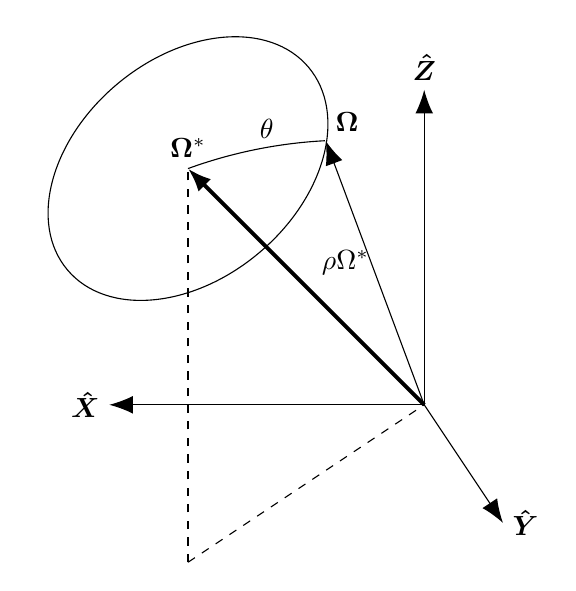
\begin{tikzpicture}
  \draw[-{Latex[length=3mm]}] (0, 0) -- (-4, 0) node[anchor=east] {$\unit X$};
  \draw[-{Latex[length=3mm]}] (0, 0) -- (1, -1.5) node[anchor=west] {$\unit Y$};
  \draw[-{Latex[length=3mm]}] (0, 0) -- (0, 4) node[anchor=south] {$\unit Z$};

  \draw[line width=0.5mm, -{Latex[length=3mm]}] (0, 0) -- (-3, 3) node[anchor=south] {$\bm \Omega^*$};
  \draw[dashed] (-3, -2) -- (-3, 3);
  \draw[dashed] (-3, -2) -- (0, 0);

  \draw[-{Latex[length=3mm]}] (0, 0) -- (-1.25, 3.35) node[anchor=south west] {$\bm \Omega$};
  \draw[rotate around={-50:(-3,3)}] (-3,3) ellipse (1.4 and 2);
  \draw (-3, 3) arc (110:93:6);
  \draw (-2, 3.5) node[anchor=center] {$\theta$};
  \draw (-1, 1.8) node[anchor=center] {$\rho \Omega^*$};

  \end{tikzpicture}
  \caption{Diagram in the inertial frame of the uncertainty model used to define the probability that the true spin vector $\bm \Omega^*$ should be observed as $\bm \Omega$. The parameter $\theta$ is drawn from a Gaussian with width $\sigma_\theta$, and $\rho$ is drawn from a log normal distribution with width $\sigma_\rho$.}
  \label{fig:uncertainty-model}
\end{figure}

The log likelihood resulting from this uncertainty model is (excluding additive constants)
\begin{equation}
  \begin{split}
  \ln \mathcal{L} = -\frac{1}{2}\sum_{i = 0}\Bigg[&\frac{\cos^{-1} (\bm \Omega_i^* \cdot \bm \Omega_i/(\Omega_i^* \Omega_i))^2}{\sigma_\theta^2}\\
  +&\frac{\ln \parens{\Omega_i /\Omega_i^*}^2}{\sigma_\rho^2} + 2\ln\frac{\Omega_i}{\Omega_i^*}\Bigg].
  \end{split}
  \label{eqn:log-likelihood}
\end{equation}
where $\Omega_i$ is the $i$th spin vector in the data set.

This model was chosen because it separates spin pole and period uncertainty. Therefore, if one is more precisely determined by measurement, $\sigma_\theta$ and $\sigma_\rho$ can be adjusted separately in accordance.





\subsection{Fit process}
\label{sec:fit}
Given synthetic data, an Affine Invariant Markov Chain Monte Carlo (MCMC) Ensemble sampler was used to generate PPDs from flat priors. We use the Python implementation \texttt{emcee} \cite{foreman2013emcee}. Our parameters were $\gamma_0$, $K_{20}$, $K_{22}$, and $K_{3m}$ (10 in total), and were bounded by $|\gamma_0| < \pi/4$, and bounds on $K_{2 m}$ given in equation \ref{eqn:parameter-bounds}. Note that $\gamma_0$ is degenerate with $\gamma_0 + \pi/2$ since this is equivalent to re-labeling $\unit y$ as $\unit x$ and $\unit x$ as $-\unit y$. The other bounds were $|K_{3m}| < 1$.

The MCMC was determined to converge when the fractional change in autocorrelation time (computed every 100 iterations) was one percent, and the number of iterations computed so far was more than 100 times the autocorrelation time. The MCMC fit also was set to terminate if more than $10^5$ iterations were run, but this only occurred for fits in which the data was too low quality to resolve the parameters. $~10^4$ iterations was often sufficient, which generally consumed about 7 hours of computation time on a super computer running 16 threads on 8 cores.

Before the MCMC was run, local minima in the likelihood were found via the Nelder-Mead algorithm implemented in \texttt{scipy} \cite{Gao2012}. It was found that only one local minimum existed, except when $K_{22}=0$ in which case rotational symmetry caused multiple values of $\gamma_0$ to be degenerate. Walkers were initialized near this local minimum, distributed with probability distributed as a Gaussian approximation of the likelihood, as determined via the inverse Hessian of the likelihood at the minimum. Due to the high sensitivity of the angular velocity data to density moments, the minimization procedure sometimes failed to isolate the minimum likelihood. Therefore, a simpler simulation without the $K_{3m}$ terms of equation \ref{eqn:tidal-torque} was first used to minimize likelihood as a function of $\gamma_0$ and $K_{2m}$, and then the full simulation was used to find $K_{3m}$, with $\gamma_0$ and $K_{2m}$ fixed. This tiered minimization process motivates us to call $\gamma_0$ and $K_{2m}$ the ``first-order parameters'' and $K_{3m}$ the ``second-order parameters.''

We further subdivided the minimization process by first minimizing with respect to data truncated at the point after perigee where $D=fr_p$ for some manually-set fraction $f$. In practice, $f=2$ often led to success. The minimum was then further refined by minimizing based on the full data, with the previous minimum as the initial estimate.





\section{Results}
\label{sec:results}

\subsection{Spin evolution}

In figure \ref{fig:example-data}, we present example spin data generated via our simulation. A population of one thousand asteroids with identical initial conditions except for $\gamma_0$, $K_{20}$, and $K_{22}$ were simulated on a close Earth encounter. The exact parameters used were the symmetric and asymmetric cases described in appendix \ref{app:reference-configs}. Bands containing 68.3\%, 95.5\%, and 99.7\% of the population's spin are shown, as is the spin of the reference asteroids in black.

\begin{figure*}
  \centering
  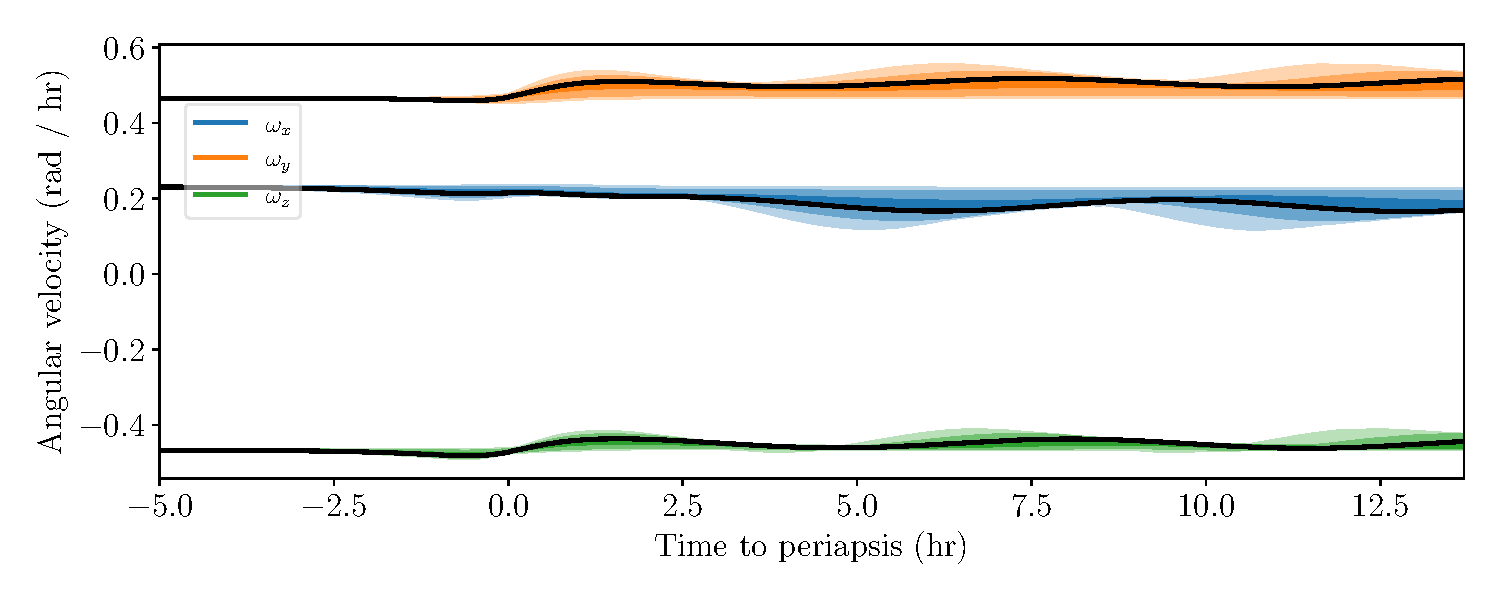
\includegraphics[width=0.7\linewidth]{figs/nominal-data-sym.pdf}
  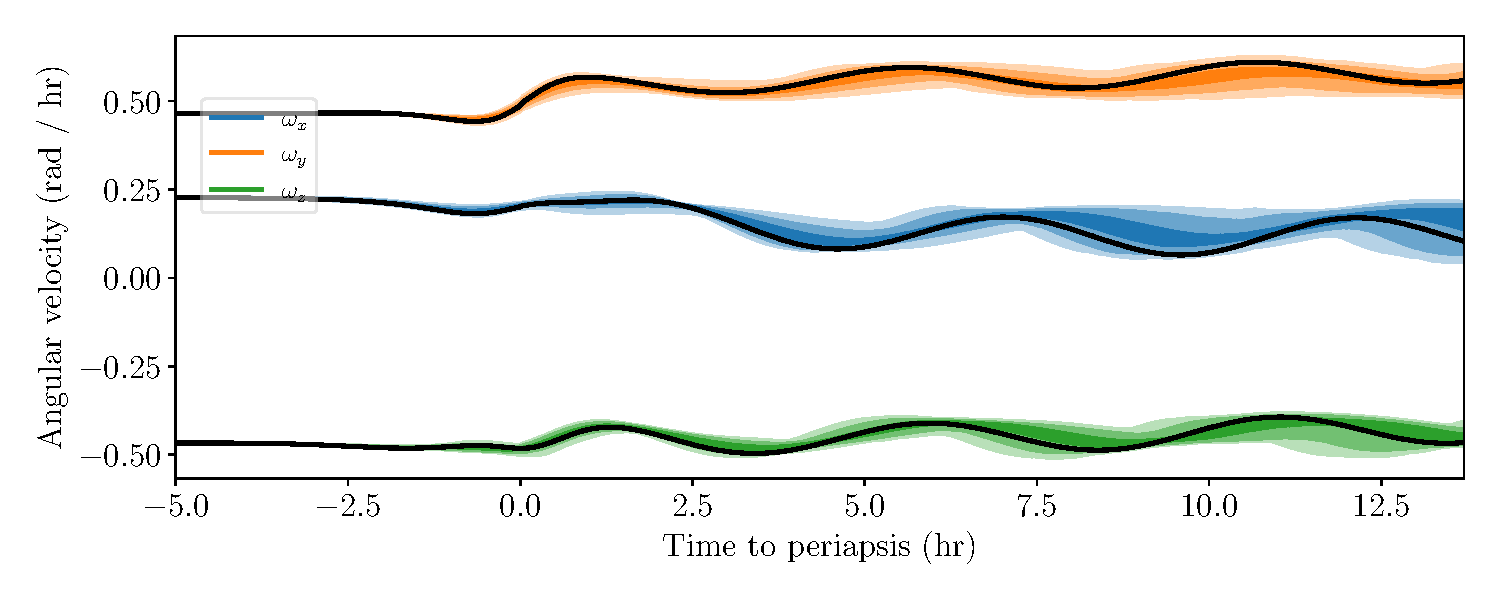
\includegraphics[width=0.7\linewidth]{figs/nominal-data-asym.pdf}
  \caption{Angular velocity data simulated for the symmetric (above) and asymmetric (below) reference asteroids. The true angular velocity evolution is shown as a black line. Also plotted is the deviation of the data for PPD-distributed perturbations to the asteroid shape (bands). Bands contain 68.3\%, 95.5\%, and 99.7\% of the 1000 simulations run.}
  \label{fig:example-data}
\end{figure*}

\begin{figure*}
  \centering
  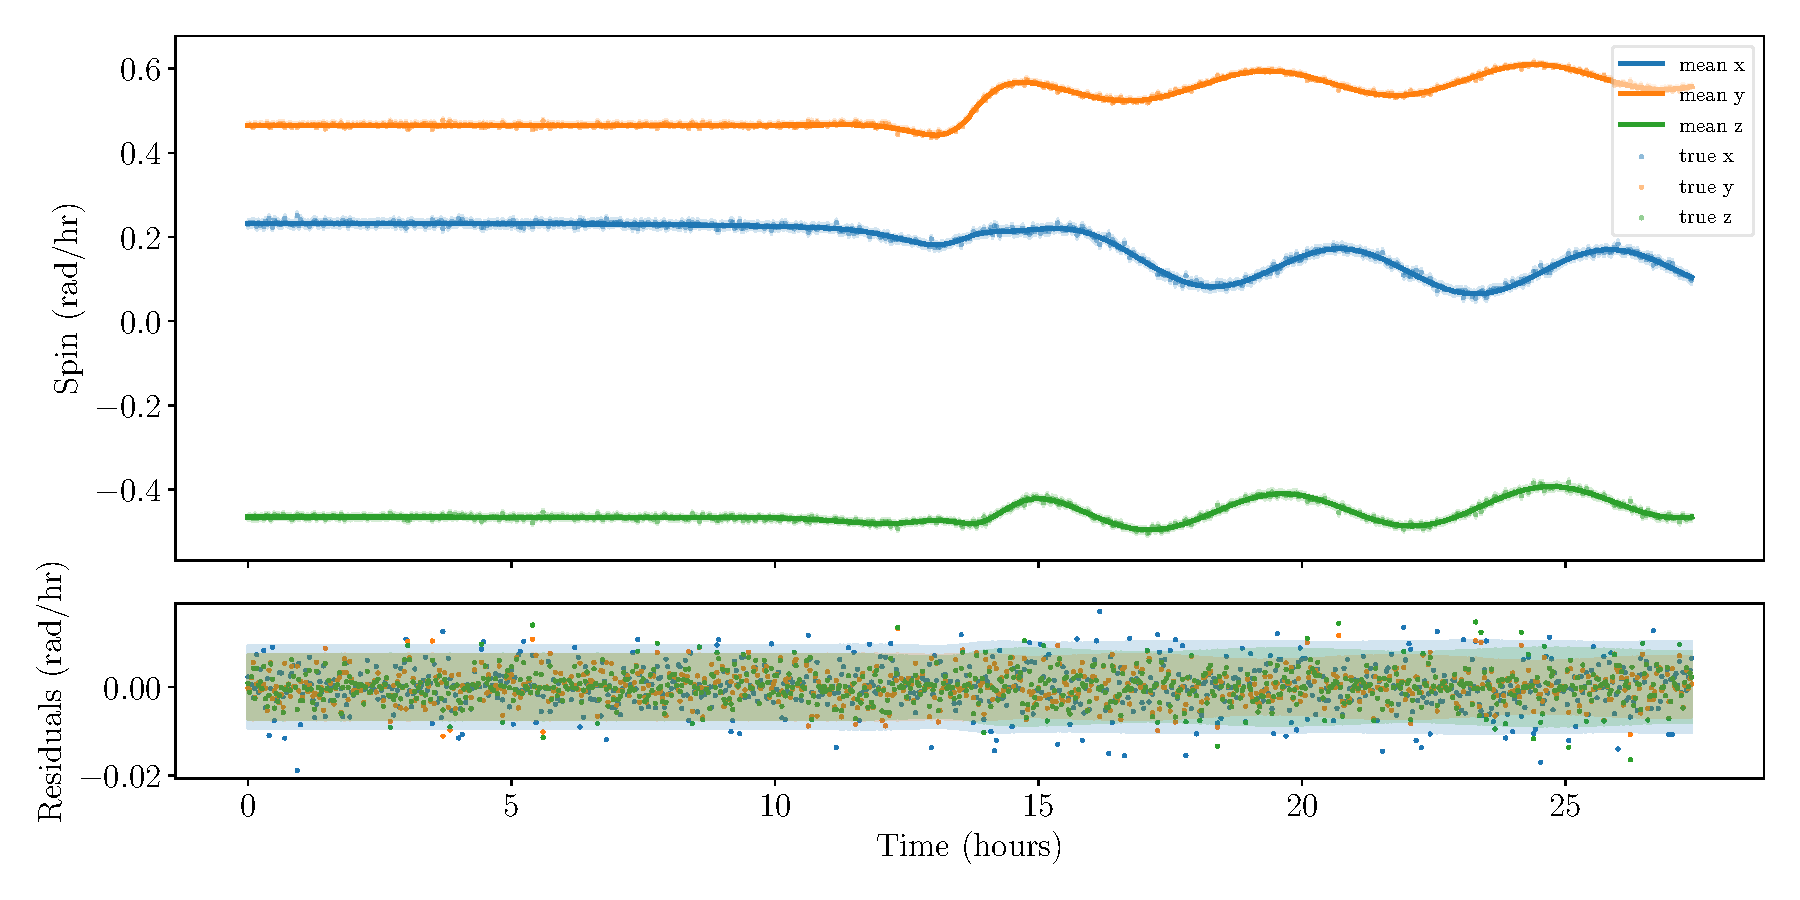
\includegraphics[width=0.7\textwidth]{figs/example-residuals.pdf}
  \caption{Data, best fit results, and residuals for a fit to synthetic data simulated for an asymmetric reference asteroid. The standard deviation of the data is plotted as an uncertainty band in the residuals plot, but these do not capture covariance between data points.}
  \label{fig:example-residuals}
\end{figure*}

To choose the initial values of $\gamma_0$, $K_{20}$, and $K_{22}$, spin data for the reference asteroids of appendix \ref{app:reference-configs} was first generated. Then $\gamma_0$, $K_{20}$, and $K_{22}$ were re-extracted via the fit described in section \ref{sec:fit}. The population's values for these parameters were PPD-distributed. However, the PPD distribution was widened by a factor of 1000 to make the band widths visible. Therefore, the scale of the bands in figure \ref{fig:example-data} have little meaning in an absolute sense, but they are meaningful when comparing two bands or two times in the same band.

The figure illustrates the sensitivity of spin data to asteroid density moments and $\gamma_0$; Before perigee, all asteroids had similar angular velocities, but after perigee the angular velocities of the population diverged. The oscillation periods observable during the torque-free precession phase of the spin data (about 5 hours after perigee) vary within the population, showing that they can be used to constrain $K_{22}$ and $K_{20}$.

\subsection{Example fit results}

Here, we present example results of the MCMC fit described in section \ref{sec:fit}, applied to encounter data of the asymmetric reference asteroid. The fit results were consistent with the true density moments, and produced consistent data.

Figure \ref{fig:example-residuals} shows the spin data with the best-fit overlaid in the top pane and the residuals in the bottom pane. Uncertainties are plotted on the residuals corresponding to the square root of the diagonal entries of the covariance matrix (correlations not included).


Figure \ref{fig:example-corner} shows a corner plot of the ten fitted parameters' posterior distributions, marginalized to functions of one or two variables. The true parameters are shown as lines. Note that the true parameters usually lie within 1- or 2$\sigma$ of the $\Delta K_{\ell m} = 0$, where $\Delta K_{\ell m}$ is the difference between the posterior $K_{\ell m}$ and the true $K_{\ell m}$.

\begin{figure*}
  \centering
  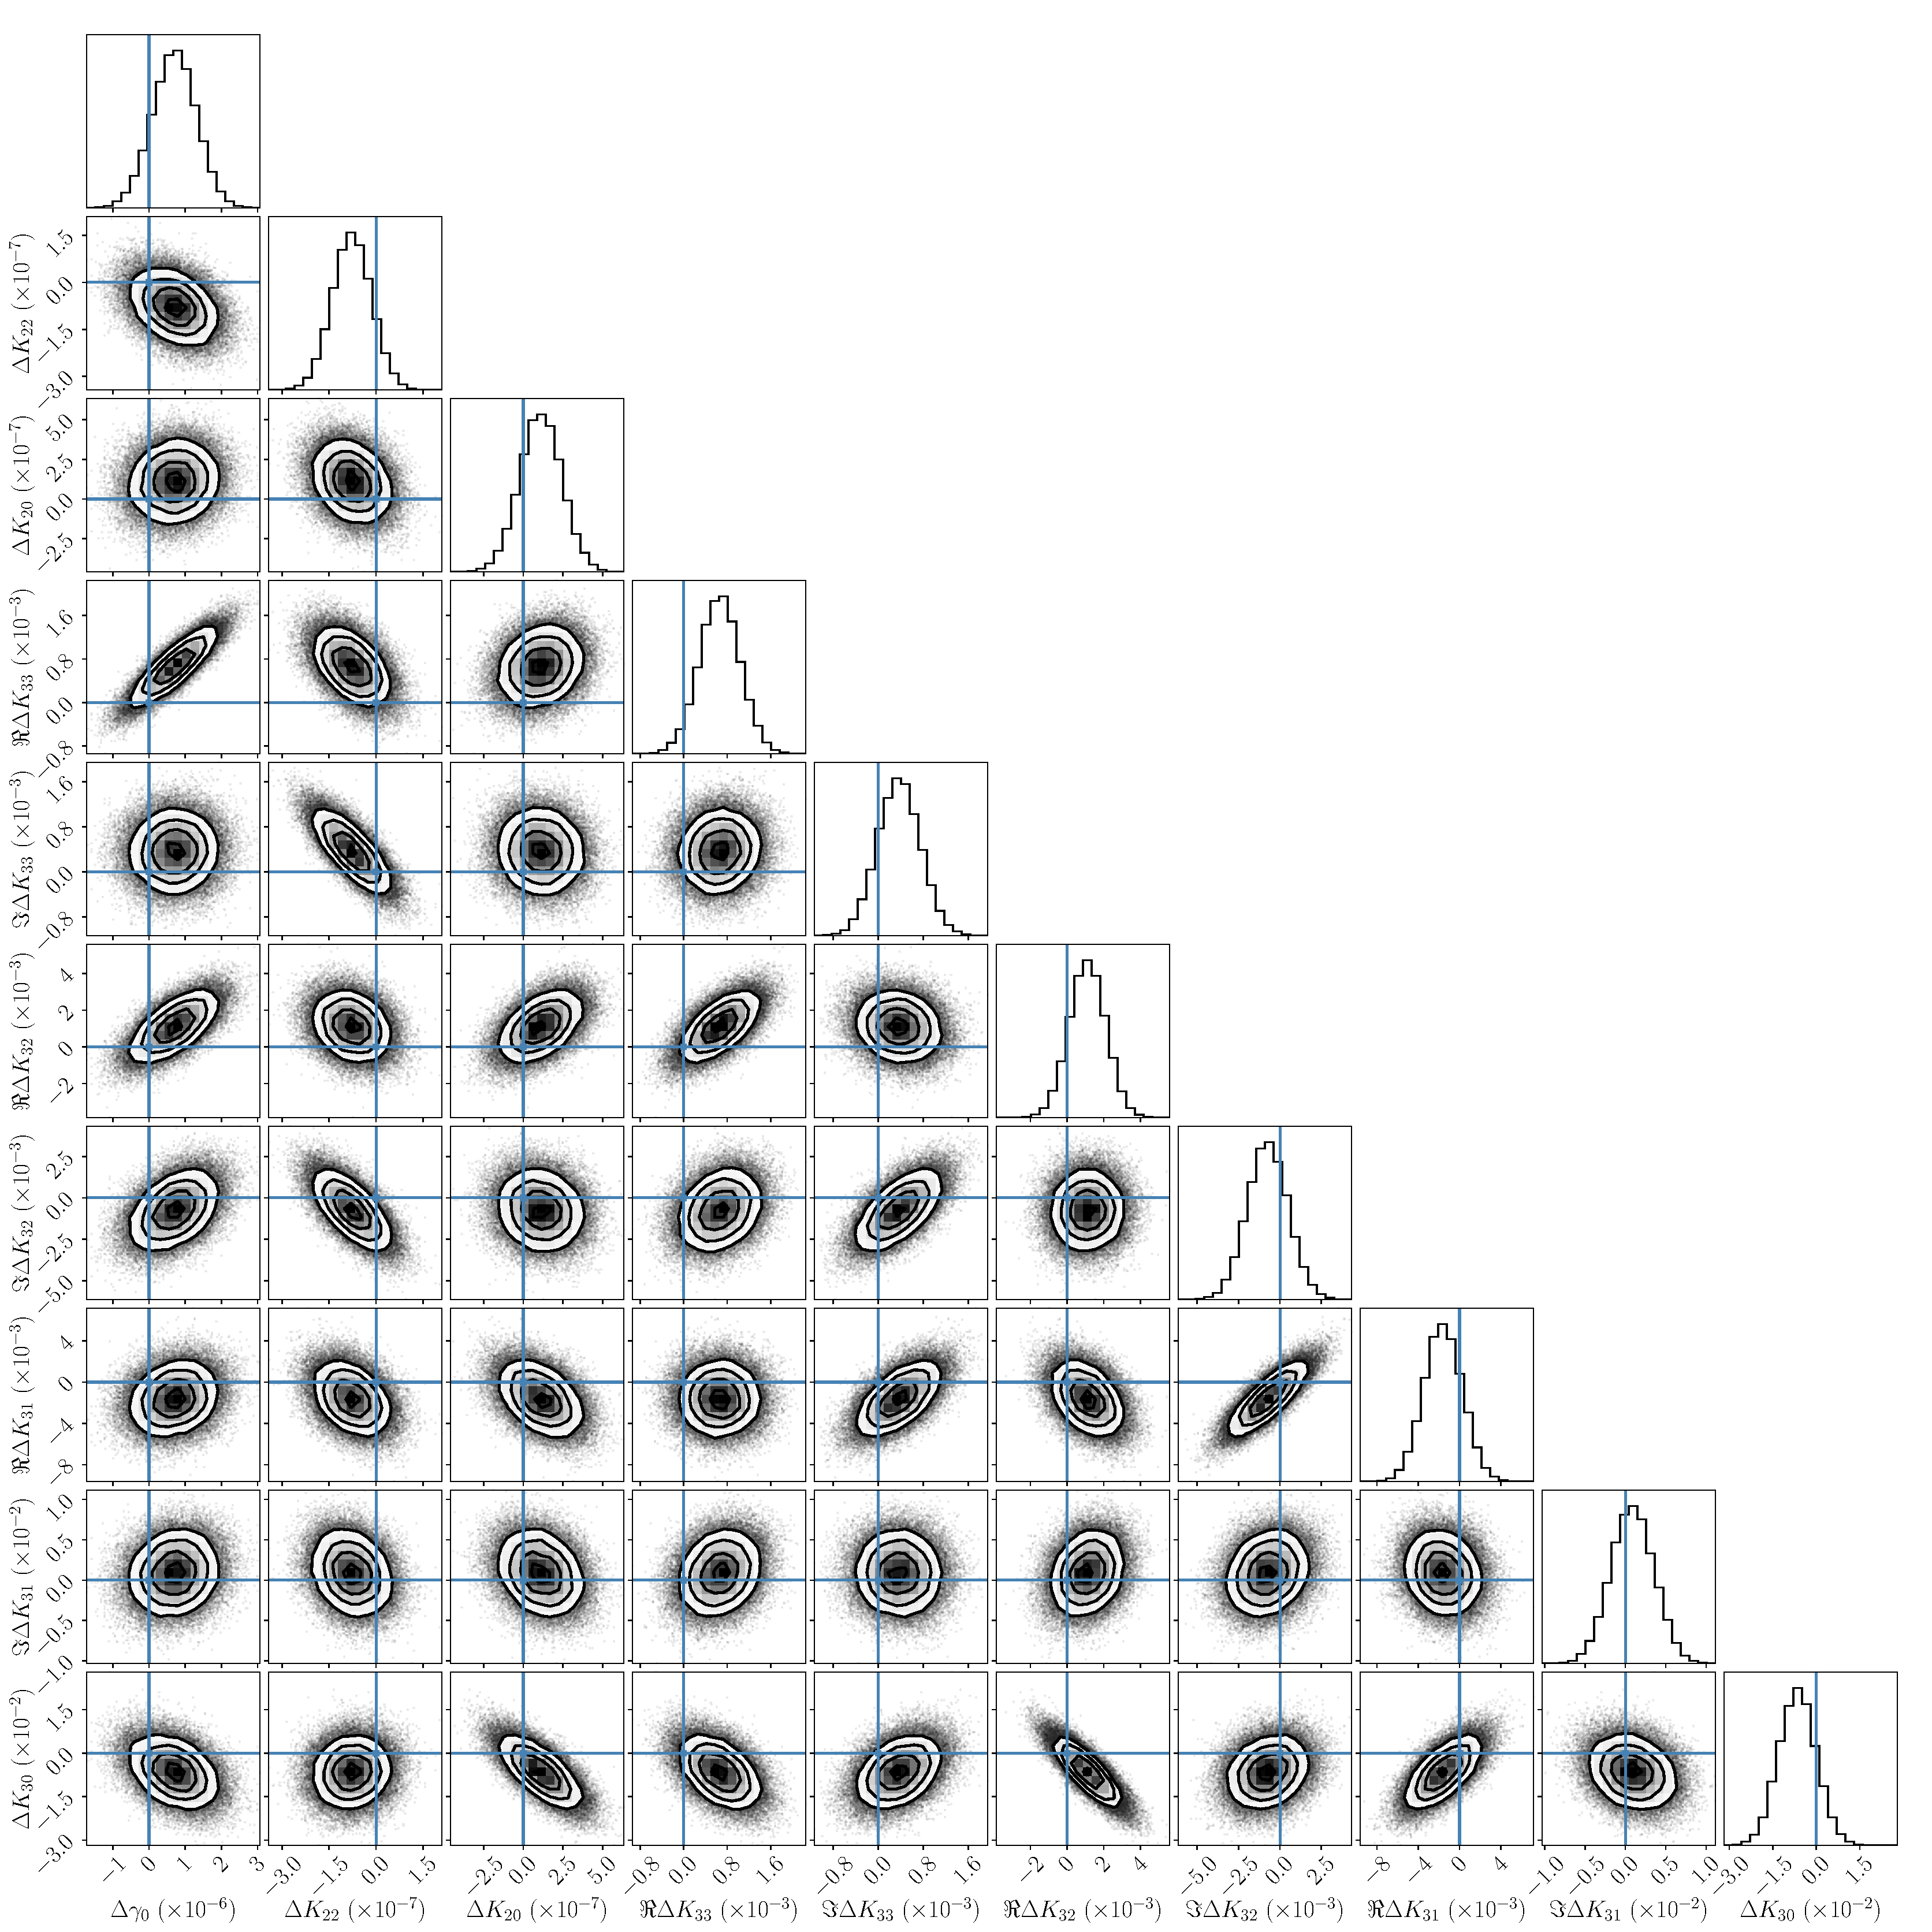
\includegraphics[width=\textwidth]{figs/example-corner.pdf}
  \caption{A corner plot for the fit results ten parameters to synthetic data simulated for an asymmetric reference asteroid. Marginal posterior PDFs for each parameter are shown (histograms) along with two-dimensional PDFs (contours). Individual points in the contours are samples from the MCMC fit, and the contours enclose 1-, 2-, and 3-$\sigma$ of them. True values (which are zero here due to the parameters being displayed relative to the true values) are also shown (blue lines).}
  \label{fig:example-corner}
\end{figure*}

\subsection{Density stuff?}




\section{Discussion}
\label{sec:discussion}


% \afterpage{
%   \begin{landscape}
%     \begin{figure}
%     \centering
%     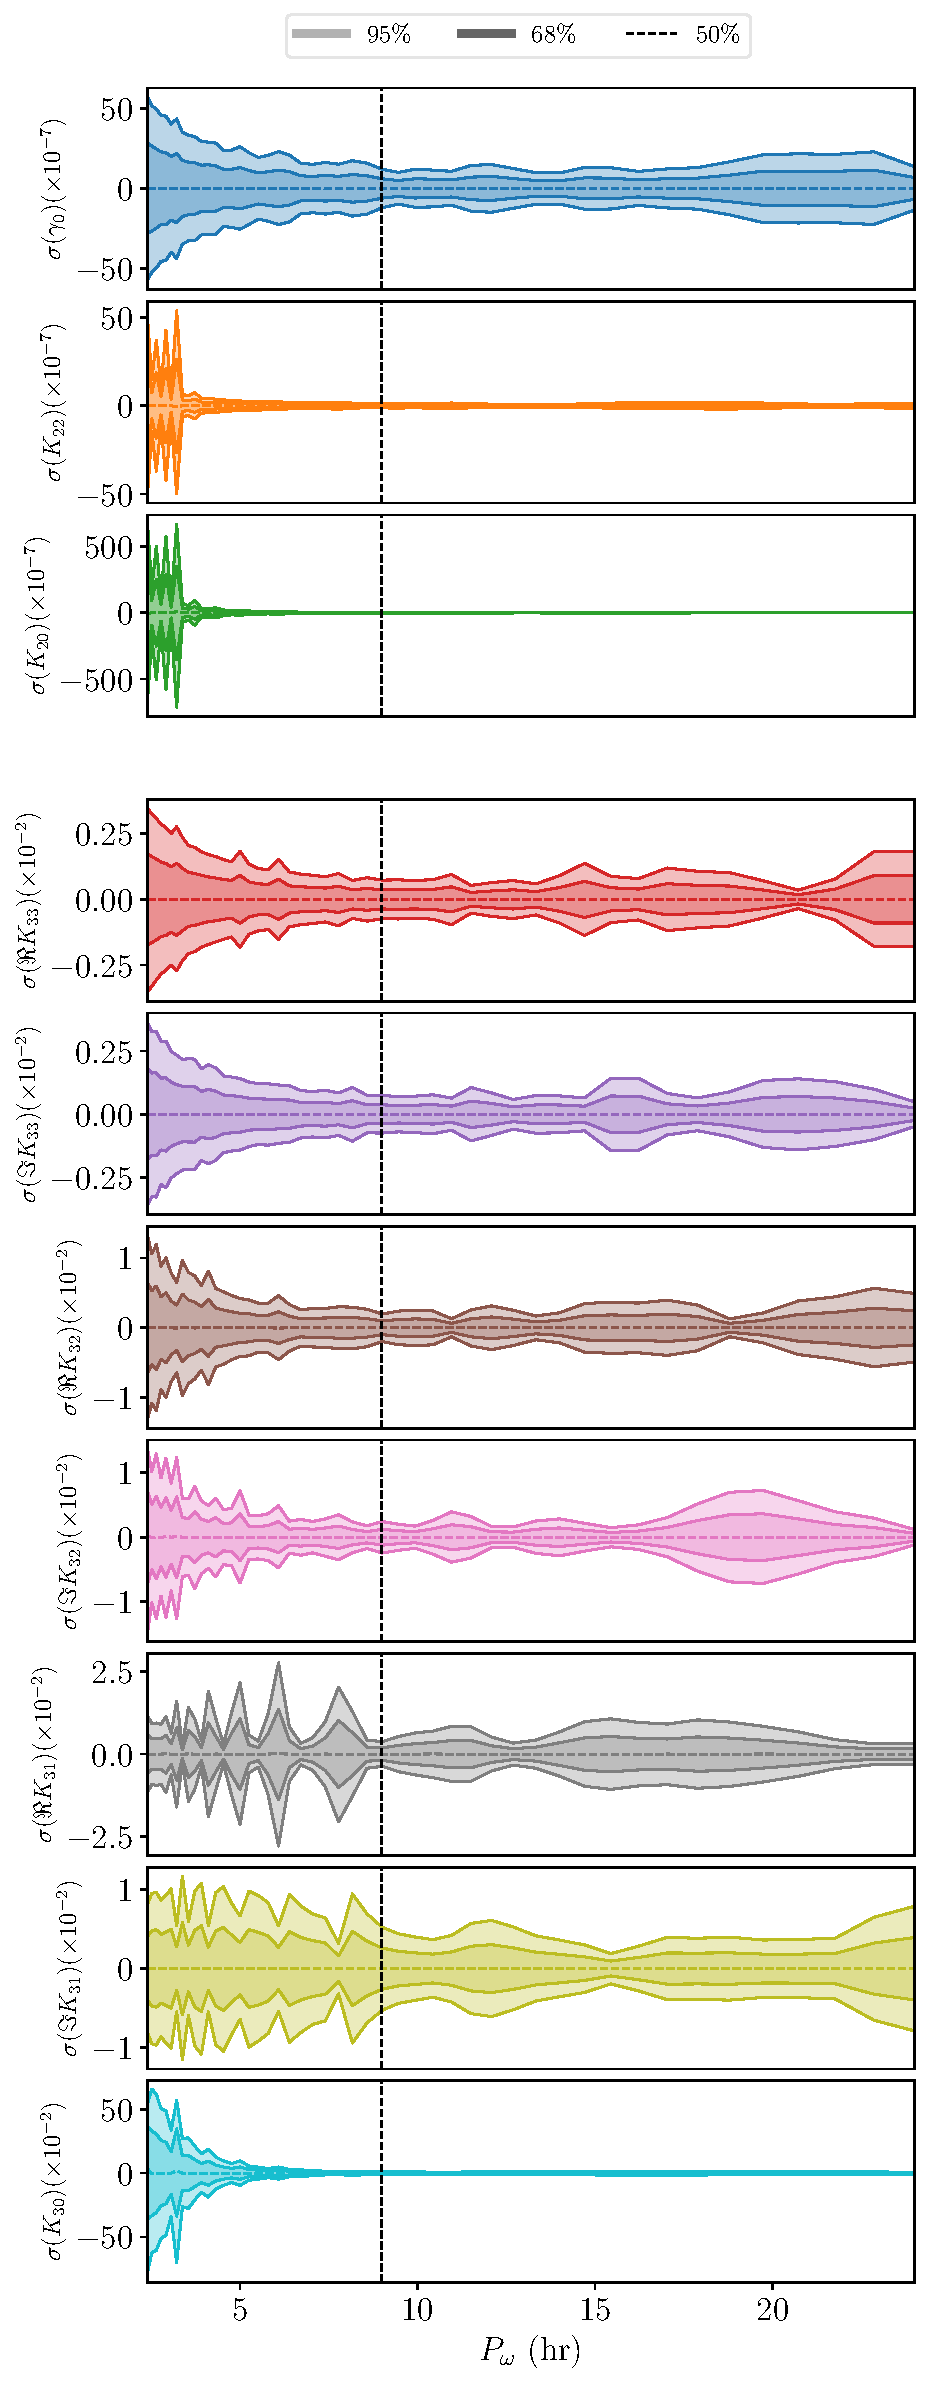
\includegraphics[height=0.89\textheight]{figs/scan-period.pdf}
%     \caption{caption}
%     \label{fig:label}
%     \end{figure}
%   \end{landscape}
% }
% PLOTS THAT COULD BE HERE
% rp
% vp


In this section, we assess the sensitivity of the PPDs for the first-order parameters ($\gamma_0$, $K_{20}$, and $K_{22}$), and the second-order parameters ($K_{3m}$) to many possible close encounter configurations. Specifically, we test sensitivity to the encounter's orbital parameters, the degree of observational uncertainty, the asteroid's radius, the cadence of observation, the amount of data collected at perigee, the direction of the initial spin pole, the asteroid period, and the central body oblateness. These effects are presented roughly in order of how much they affect the parameter precision, from highest to lowest.

Parameter precision of 1$\sigma$ is defined such that 68.27\% of the PPD lies within 1$\sigma$ of the mean of the PPD. 2$\sigma$ is defined likewise for 95.45\% of the PPD. The PPDs are usually roughly Gaussian, so that the upper and lower error bars are usually roughly equal and 1$\sigma$ is approximately the standard deviation of the PPD.

In all cases, we use the configuration of the asymmetric reference asteroid (appendix \ref{app:reference-configs}) unless otherwise stated. We further present a test of how precision depends on cadence, asteroid period, and the duration of the encounter in appendix \ref{app:cadence-tests}, and we compare precision for a Jupiter and an Earth encounter in appendix \ref{app:jupiter-earth}.


\subsection{Orbital elements}
\label{sec:scan-orbit}
A Keplerian orbit is completely described by five parameters, but three describe the orbit's orientation with respect to the central body. The orbit can be rotated to the $\unit X \unit Y$-plane, as mandated by our coordinate definitions, by changing the density moments of the central body. Since $J_{00}$ is unchanged by this rotation and $J_{1m}=0$, the orbit orientation is irrelevant until the $J_{2m}$ terms of equation \ref{eqn:tidal-torque}, and we do not investigate them here.

We parametrize the shape of the orbit by the perigee distance $r_p$ and excess velocity $v_\infty$. Fits of the type described in section \ref{sec:fit} were run for many values of $r_p$ and $v_\infty$ and the 1 and 2$\sigma$ confidence intervals are displayed in figures \ref{fig:scan-vex} for $v_\infty$ and \ref{fig:scan-perigee} for $r_p$.



\begin{figure}
  \centering
  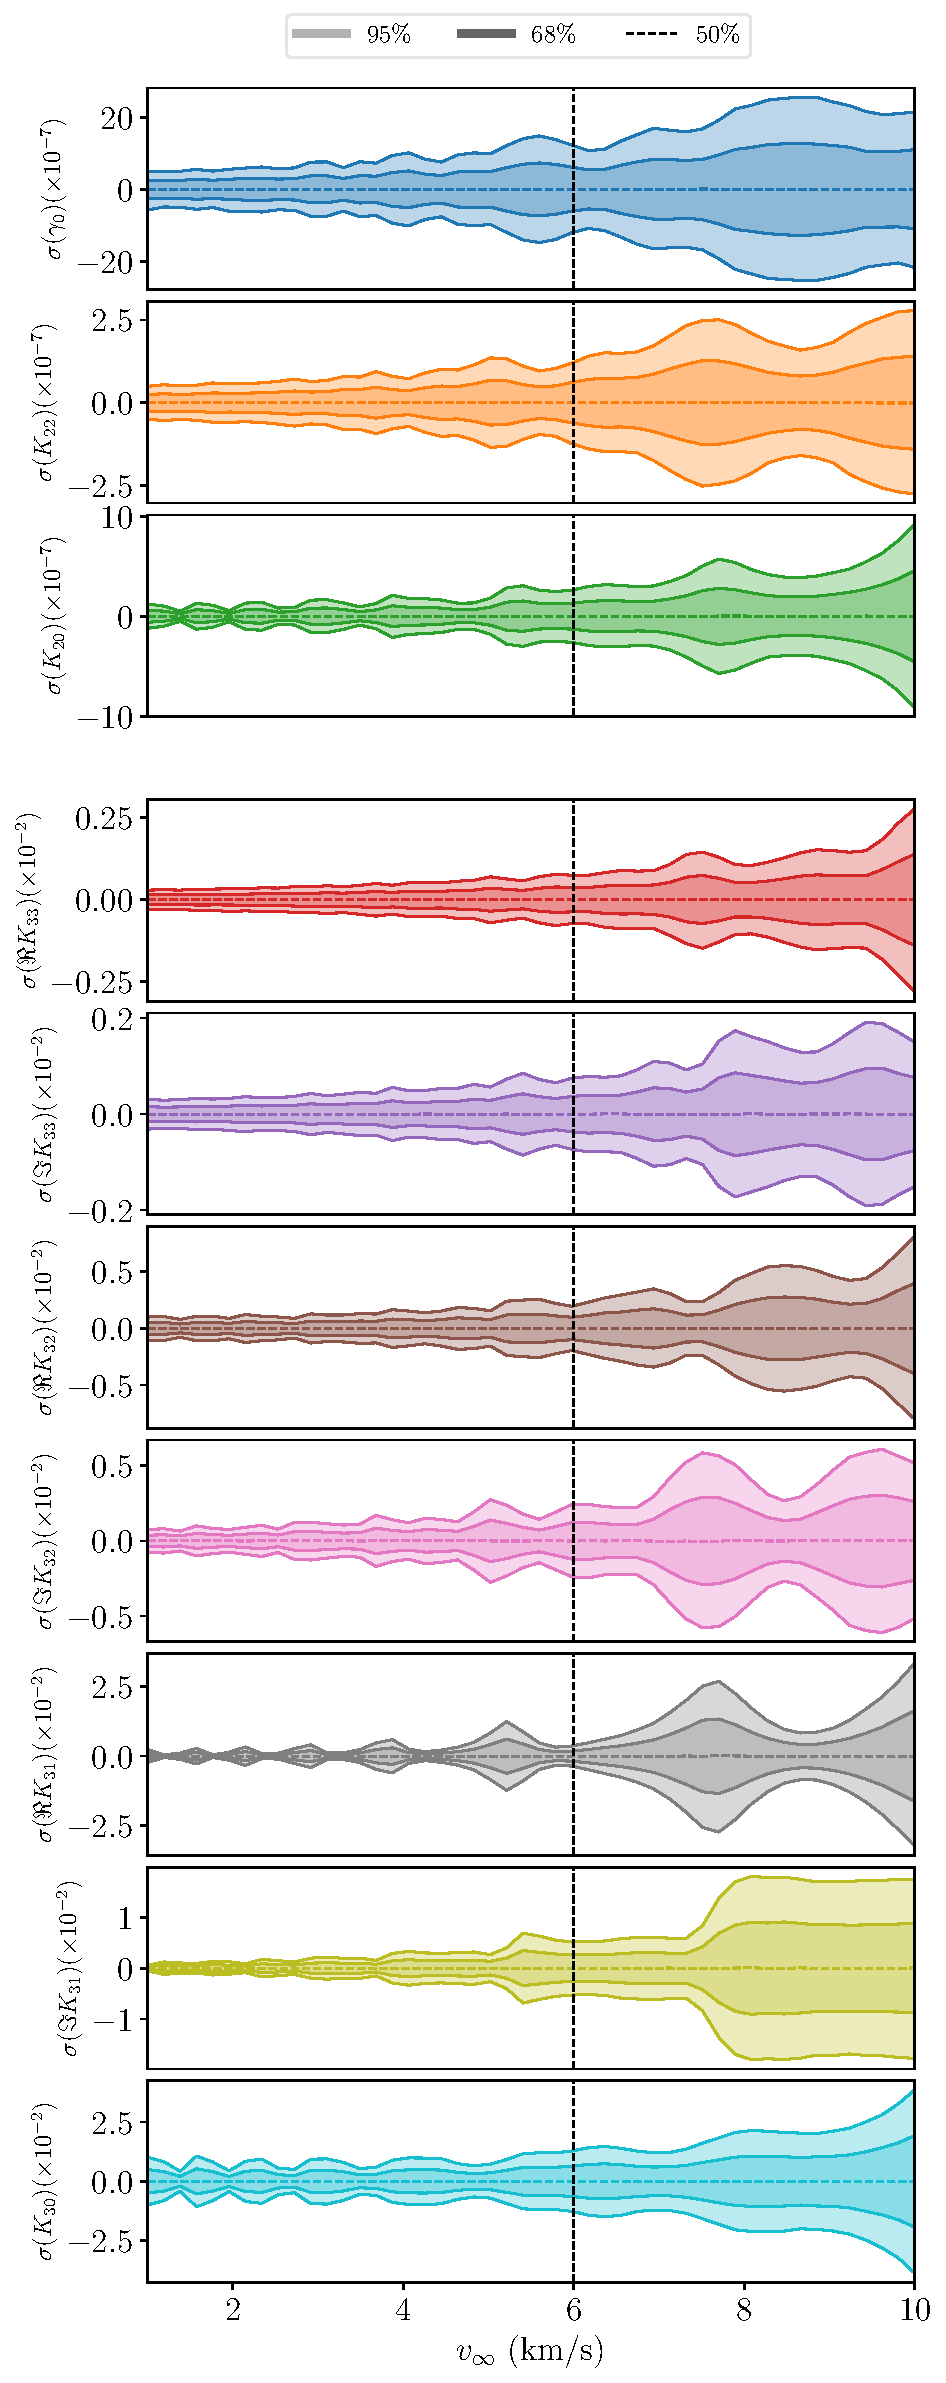
\includegraphics[height=0.89\textheight]{figs/scan-vex.pdf}
  \caption{1 and 2$\sigma$ confidence intervals for the first-order parameter PPDs (\textit{top}) and second-order parameters (\textit{bottom}) as a function of orbital excess velocity $v_\infty$. The vertical dashed line indicates the reference asteroid value of 6 km s$^{-1}$. The red vertical lines indicate when $\sigma = 0.01$.}
  \label{fig:scan-vex}
\end{figure}

Figure \ref{fig:scan-vex} demonstrates that parameter precision does not depend strongly on excess velocity, aside from a slight trend especially in the higher order parameters for uncertainty to increase with $v_\infty$. This is likely due to the fact that larger $v_\infty$ leads to a faster and flatter orbit with less time spent close to the planet, where tidal torque is strongest. There are also smaller-scale oscillations in the uncertainty, due to the orientation of the asteroid at perigee varying. The asteroid is always simulated to start at the same orientation, but increasing $v_\infty$ decreases the time to perigee, so that the asteroid enters this region of high torque at different orientations depending on $v_\infty$. This effect explains why these small-scale oscillations have the same period for all parameters. Note that these oscillations are sometimes large enough to raise $\sigma > 0.01$, shown by the red vertical line.

\begin{figure}
  \centering
  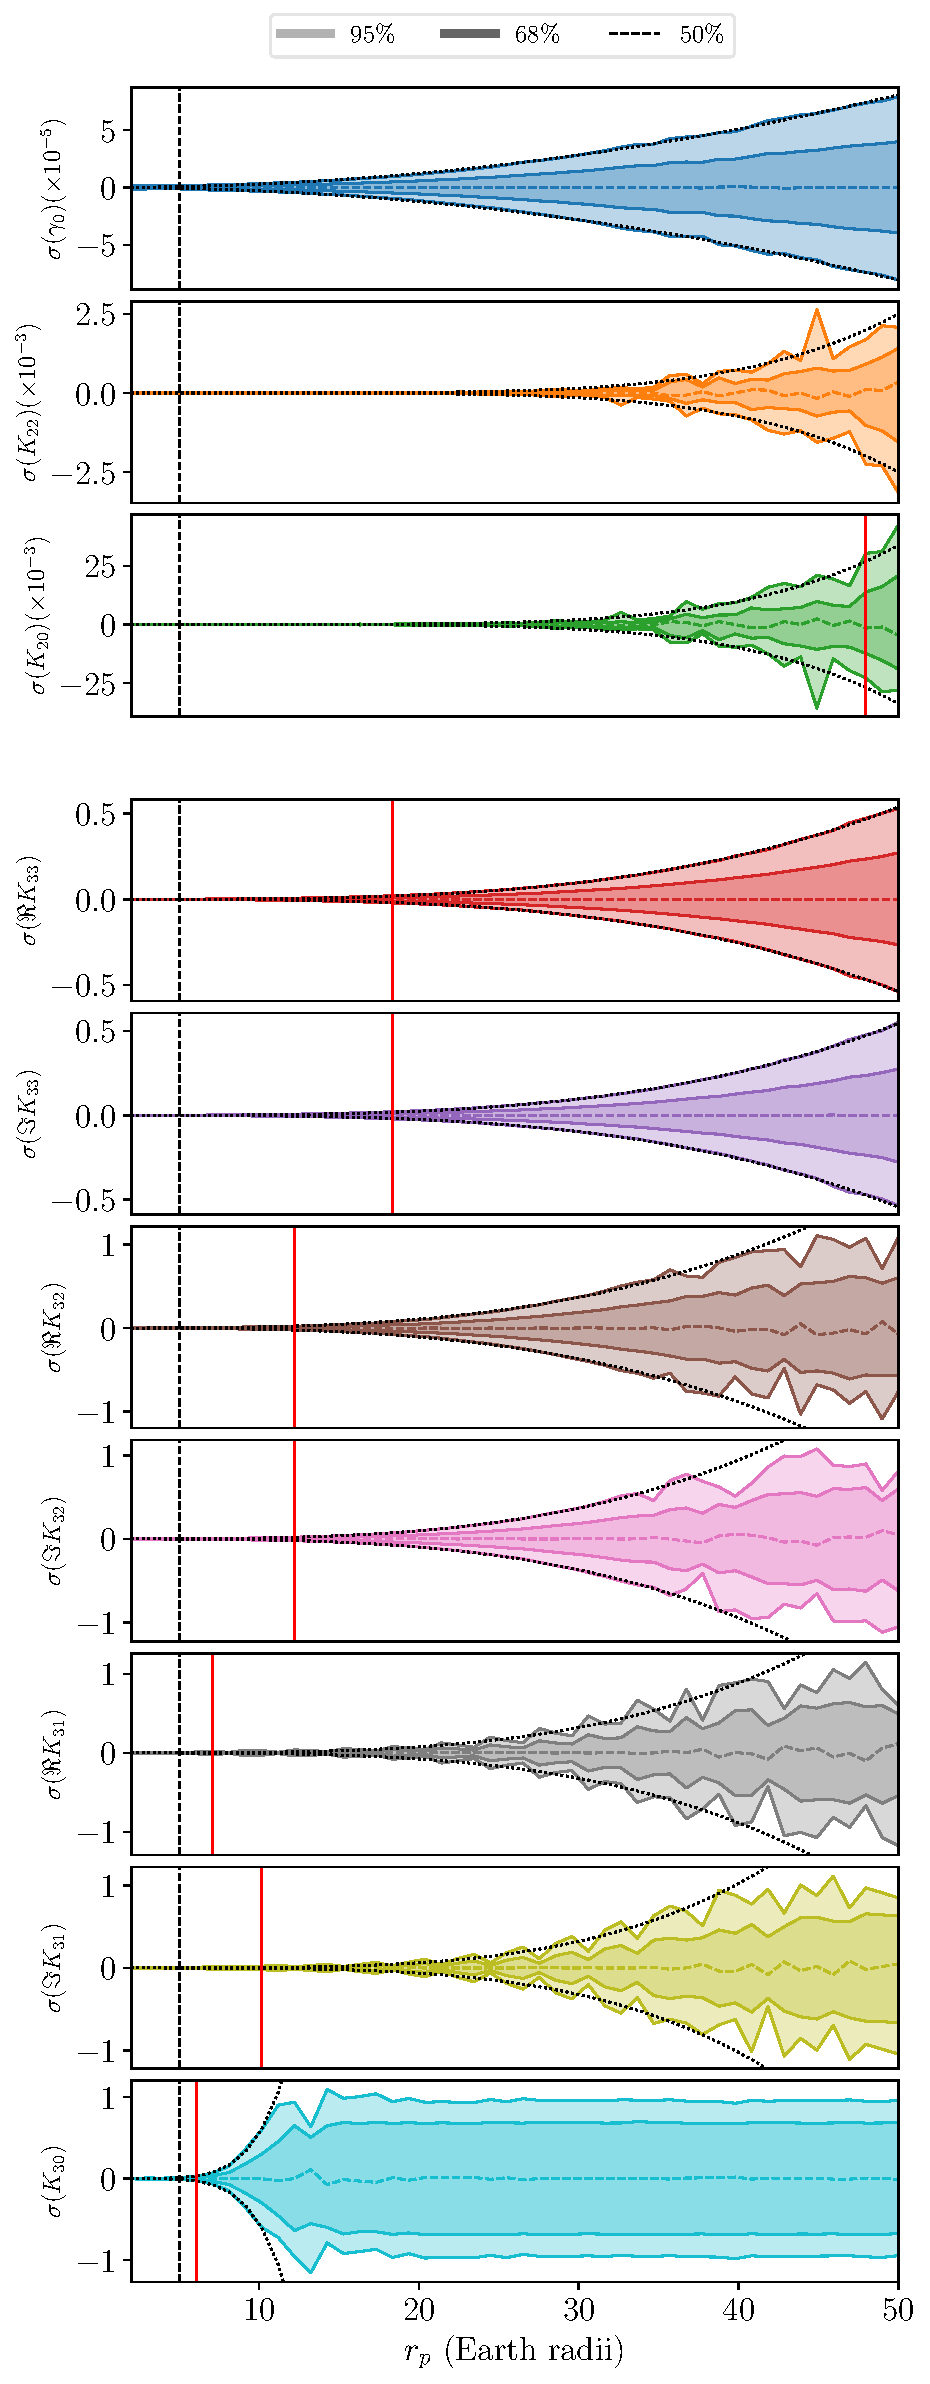
\includegraphics[height=0.89\textheight]{figs/scan-perigee.pdf}
  \caption{1 and 2$\sigma$ confidence intervals for the first-order parameter PPDs (\textit{top}) and second-order parameters (\textit{bottom}) as a function of perigee distance $r_p$. The vertical dashed line indicates the reference asteroid value of 5 Earth radii. The dotted curve indicates a power-law fit (see text). The red vertical lines indicate when $\sigma = 0.01$.}
  \label{fig:scan-perigee}
\end{figure}

Figure \ref{fig:scan-perigee} shows much stronger dependence of parameter uncertainty on perigee distance, as expected by the factor of $(a_\mathcal{A}/D)^{\ell'}$ present in equation \ref{eqn:tidal-torque} and mentioned in section \ref{sec:tidal-torque}. For $r_p \approx 6$ or 7 Earth radii, $\sigma(K_{30})$ reaches the reference 0.01 limit. At slightly higher $r_p$, $K_{31}$ and $K_{32}$ become similarly unresolved, and at $r_p \approx 20$ Earth radii, $K_{33}$, the last second-order component, becomes unresolved. Even before this, at $r_p \approx 10$ Earth radii, the most uncertain parameter $K_{30}$ fills the prior distribution with uncertainty ranging from -1 to 1, visible by the sudden cut-off in uncertainty increase and the discontinuity of the $\sigma$ curve there. The location of these limits will change if different encounter properties are used, but this is still an illustrative example.

\begin{table}
  \centering
  \begin{tabular}{l|c}
    \hline
    Parameter & $\alpha$ \\ \hline
    $\gamma_0$ & $2.05$ \\
    $K_{22}$ & $5.47$ \\
    $K_{20}$ & $5.47$ \\ \hline
    $\Re K_{33}$ & $3.35$ \\
    $\Im K_{33}$ & $3.37$ \\
    $\Re K_{32}$ & $3.05$ \\
    $\Im K_{32}$ & $3.27$ \\
    $\Re K_{31}$ & $3.53$ \\
    $\Im K_{31}$ & $4.02$ \\
    $K_{30}$ & $5.75$ \\ \hline
  \end{tabular}
  \caption{Power law slope values for the dependence of parameter uncertainty on perigee distance $r_p$. Slope is defined by $\sigma \propto r_p^\alpha$.}
  \label{tab:scan-perigee-alpha}
\end{table}

Fitted to each of the curves in figure \ref{fig:scan-perigee} are power law uncertainties $\sigma \propto r_p^\alpha$. These fits were performed via the method of least squares, and all data with $\sigma > 0.7$ was removed due to its sensitivity to the arbitrarily-chosen boundary of the prior. The values of $\alpha$ are shown in table \ref{tab:scan-perigee-alpha}. These slope values express how much each parameter is dependent on $r_p$. It is observed that $\gamma_0$ is least dependent on $r_p$, with $\sigma(\gamma_0) \sim r_p^2$. The other two first-order parameters are much more strongly dependent, with $\sigma \sim r_p^{5.5}$. The second-order parameters have milder slopes between 3 and 4 (except for $K_{30}$) which is fortunate from the perspective of making precise observations, since lower $\alpha$ renders larger values of $r_p$ accessible to measuring $K_{3m}$.

The axes of figure \ref{fig:scan-perigee} show that parameters with large $m$ are more precisely determined than parameters with small $m$, as can be seen by comparing $K_{22}$ to $K_{20}$ and comparing $K_{33}$ to other $K_{3m}$ values. Large $m$ moments correspond to moments that control higher frequency fluctuations in density at the asteroid equator. This pattern of large $m$ corresponding to low uncertainty is a general trend and will be seen in the following sections as well.

The very strong dependence of $\sigma$ on $r_p$ makes this analysis only to extract second-order moments on close encounters. Fortunately, in the case of Earth, these encounters are also likely to have the best associated observational uncertainty when above the horizon due to their proximity. The first-order moments can still be extracted at much larger perigee distances in our model.


\subsection{Observational Uncertainty}
\label{sec:scan-uncertainty}
There are two parameters, $\sigma_\theta$ and $\sigma_\rho$, which govern the observational uncertainty of the data set (defined in section \ref{sec:uncertainty}). Rather than explore the full space spanned by these two values, we measure how parameter uncertainties depend on the product of uncertainties $\sigma_\theta\sigma_\rho$ (with the radio fixed), and the ratio $\sigma_\rho / \sigma_\theta$ (with the product fixed).

We choose these metrics because we generally expect that the parameter uncertainty $\sigma$ be proportional to the observational uncertainty, but whether the dependence is stronger on $\sigma_\theta$ or $\sigma_\rho$ is not immediately clear. We get around this problem by varying $\sigma_\theta$ and $\sigma_\rho$ together and fixing their ratio, and measuring the posterior uncertainty $\sigma$, with $\sigma/\sigma_\theta$ shown in figure \ref{fig:scan-product}. Indeed, we find that $\sigma \propto \sigma_\theta$ almost exactly, and since $\sigma_\rho / \sigma_\theta$ is fixed, we also have $\sigma \propto \sigma_\rho$. For large $\sigma_\theta \sigma_\rho$, the proportionality fails, but this is because $\sigma(K_{30}) \approx 1$ which fills the prior. Uncertainty cannot increase beyond this value.

\begin{figure}
  \centering
  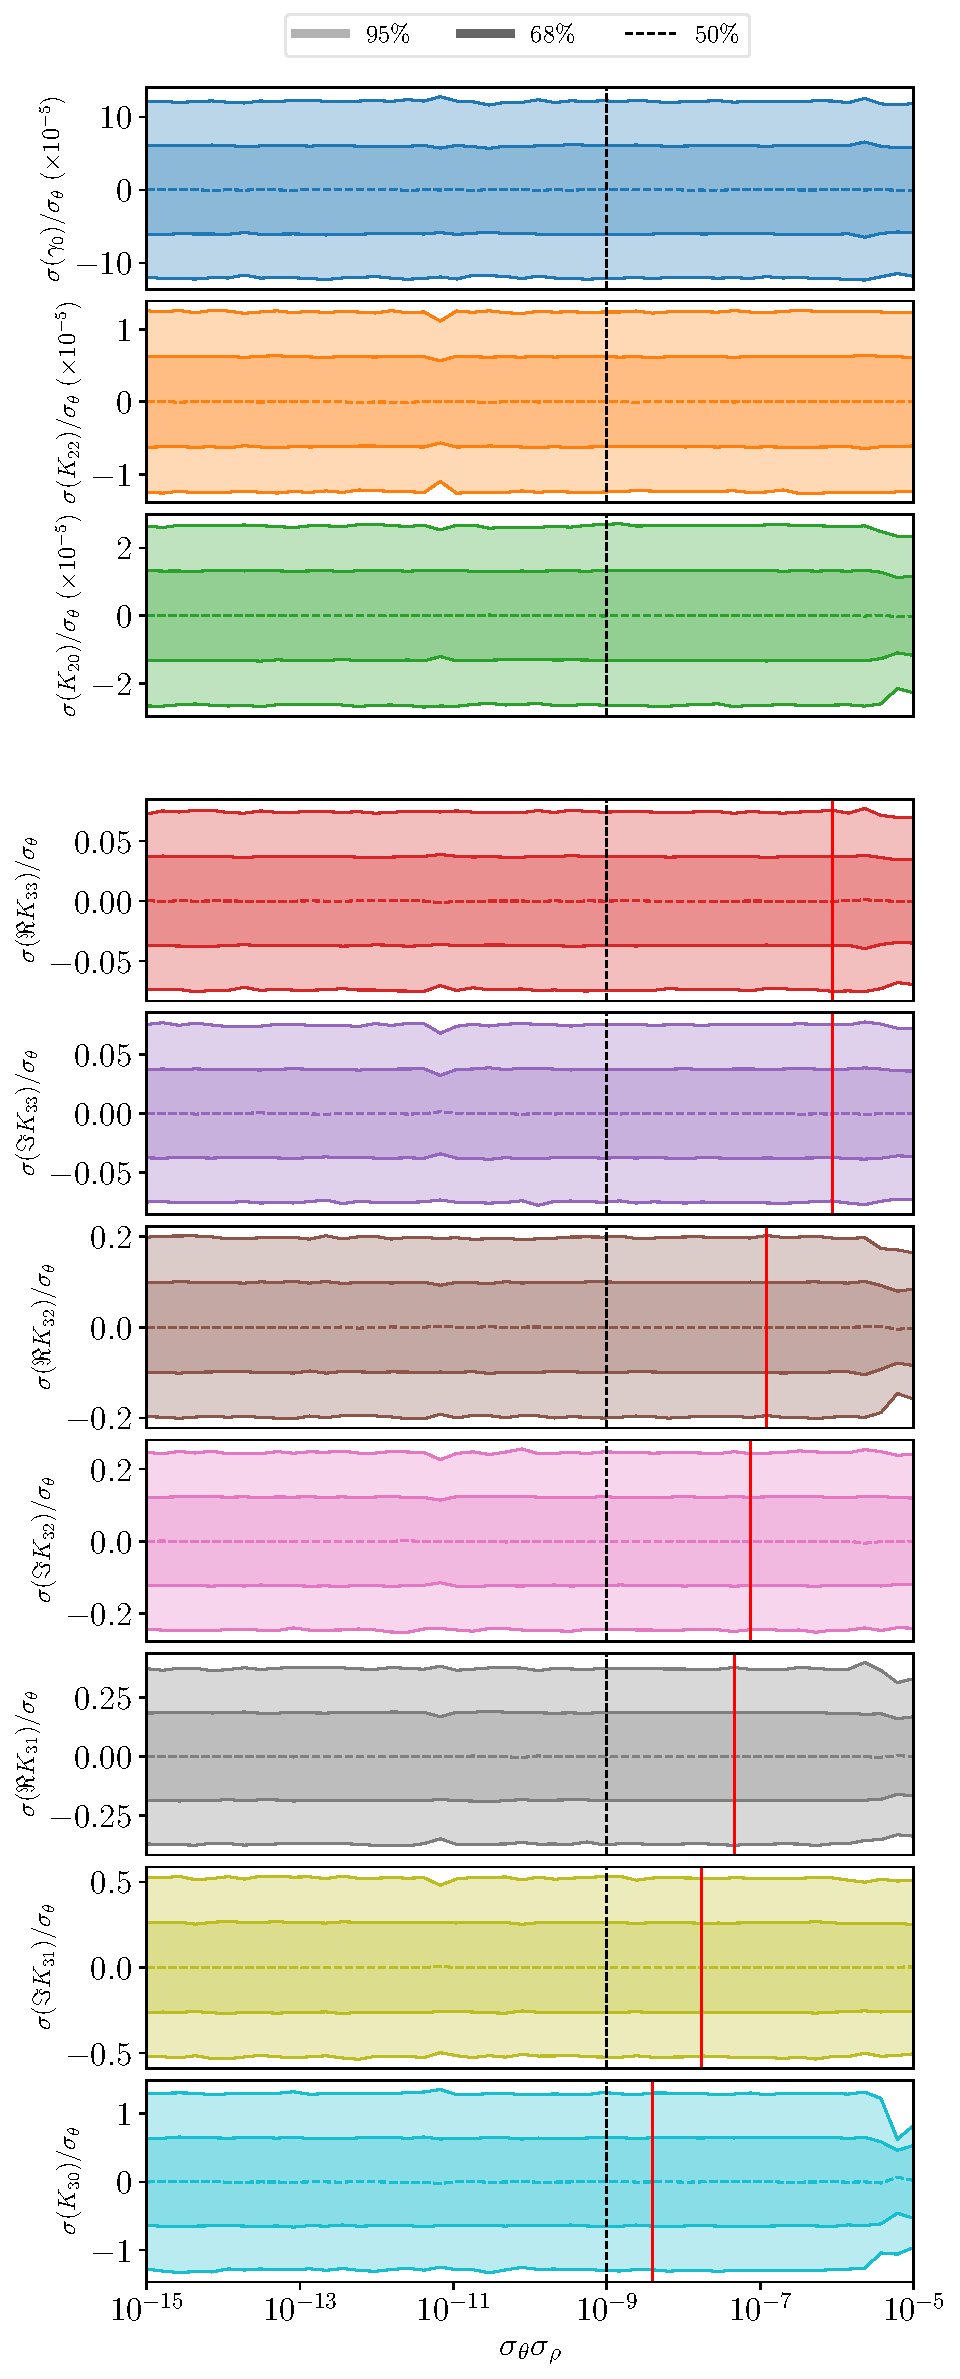
\includegraphics[height=0.89\textheight]{figs/scan-product.pdf}
  \caption{1 and 2$\sigma$ confidence intervals divided by $\sigma_\theta$ for the first-order parameter PPDs (\textit{top}) and second-order parameters (\textit{bottom}) as a function of observational uncertainty product $\sigma_\theta \sigma_\rho$. The vertical dashed line indicates the reference asteroid value of $10^{-9}$. The red vertical lines indicate when $\sigma =0.01$.}
  \label{fig:scan-product}
\end{figure}

We also investigate the dependence of posterior uncertainty on $\sigma_\rho / \sigma_\theta$ with $\sigma_\theta \sigma_\rho$ fixed in figure \ref{fig:scan-ratio}. If we simply had $\sigma \propto \sigma_\theta \sigma_\rho$, then $\sigma$ would have no dependence on $\sigma_\rho / \sigma_\theta$. Any deviation from constant $\sigma$ shown in the figure therefore reveals some additional dependence in the model on one of the observational uncertainties.

\begin{figure}
  \centering
  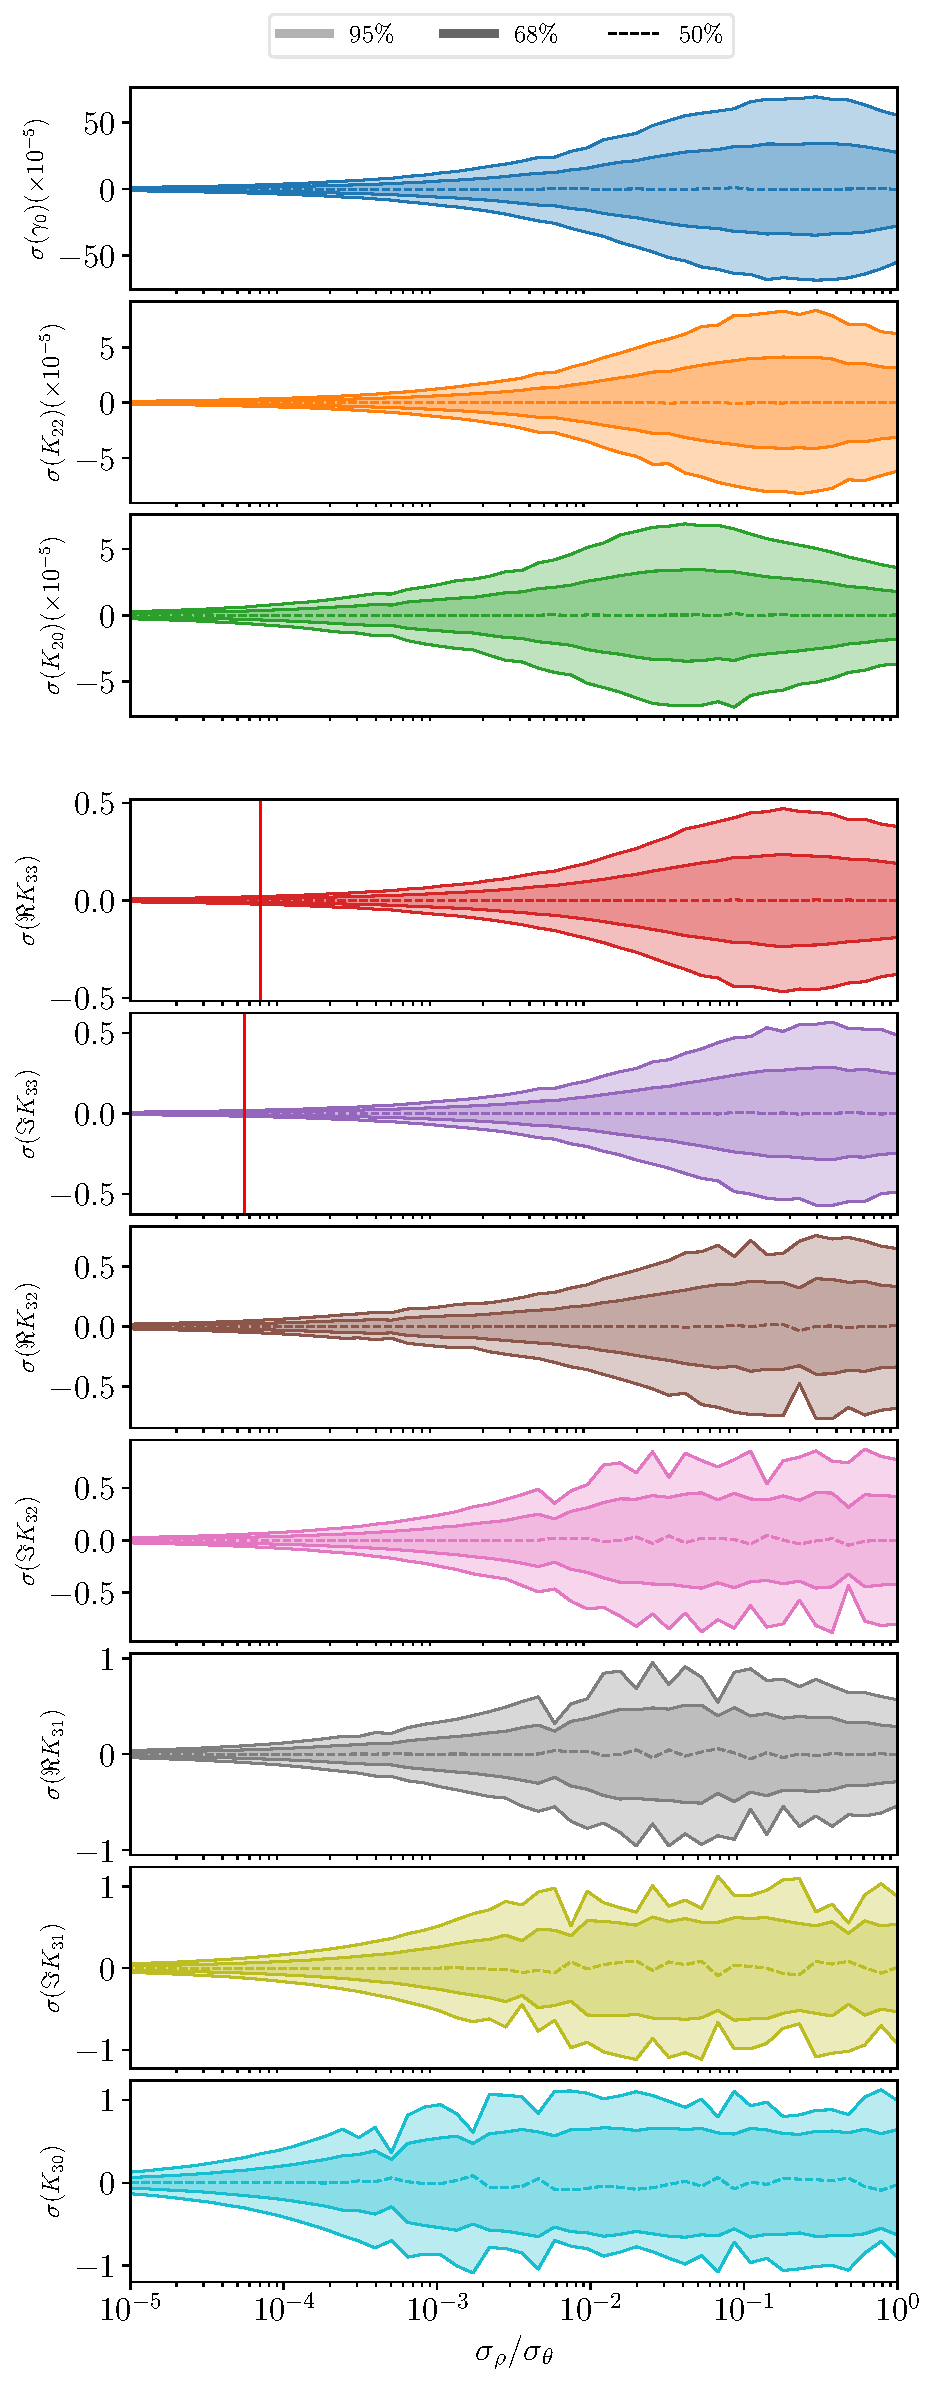
\includegraphics[height=0.89\textheight]{figs/scan-ratio.pdf}
  \caption{1 and 2$\sigma$ confidence intervals for the first-order parameter PPDs (\textit{top}) and second-order parameters (\textit{bottom}) as a function of observational uncertainty ratios $\sigma_\rho / \sigma_\theta$. The reference asteroid value is $\sigma_\rho/ \sigma_\theta =10^{-5}$. The red vertical lines indicate when $\sigma = 0.01$. (Lines are not shown for $K_{3m}$, $m < 3$ because they coincide with the vertical axis.)}
  \label{fig:scan-ratio}
\end{figure}

Indeed, figure  \ref{fig:scan-ratio} shows increased uncertainty when $\sigma_\rho/\sigma_\theta$ is large, so that $\sigma$ depends more on $\sigma_\rho$ than on $\sigma_\theta$. We summarize this pattern by stating that, if the observer had to choose between better precision on the period or on the spin pole of the data, they should choose period. This is fortunate for observers since, \jtd{I want to say that precision on the period is better constrained by light curve analysis, but I do not know enough about light curve analysis to be sure.}

Another conclusion that can be drawn from figure \ref{fig:scan-ratio} is that $\sigma(\sigma_\rho/\sigma_\theta)$ is proportional for all $K_{\ell m}$. The proportionality constant shows the same dependence on $\ell$ and $m$ mentioned previously. The proportionality is broken near $\sigma \approx \pm 1$, where $\sigma$ fills the prior.

The location of the $\sigma > 0.01$ limit demonstrates the great influence of observational precision on fit uncertainty; increasing $\sigma_\theta \sigma_\rho$ or $\sigma_\rho / \sigma_\theta$ by even a small amount raises $\sigma(K_{3m}) > 0.01$ in most cases.



\subsection{Asteroid shape}
\label{sec:scan-shape}

The true values of $K_{\ell m}$, $\gamma_0$, and $a_\mathcal{A}$ affect the uncertainties in extracted density moments $\sigma$. Here, we only investigate the sensitivity of $\sigma$ to the first-order parameters and $a_\mathcal{A}$. The $K_{2m}$ moments can therefore also be viewed as the axes of a uniform density triaxial ellipsoid (equation \ref{eqn:ellipsoid-axes}).

In figure \ref{fig:scan-space-sigma}, we show the 1$\sigma$ confidence intervals as a function of $K_{20}$ and $K_{22}$, or alternatively $a/c$ and $b/c$. We use axis ratios rather than the values of $a$, $b$, and $c$ to remove the $a_\mathcal{A}$ dependence of equation \ref{eqn:ellipsoid-axes}. The figure shows large uncertainty in $\gamma_0$ for $K_{22}=0$, or $a/c=b/c$, because $K_{20}$ is rotationally symmetric around $\unit z$, and $\gamma_0$ is the initial orientation with respect to the $\unit z$ axis. The data then have no physical dependence on $\gamma_0$ when $K_{22}=0$. This induces degeneracy in the model which inflates uncertainties, not only in $\gamma_0$ but also the other components.

\begin{figure*}
  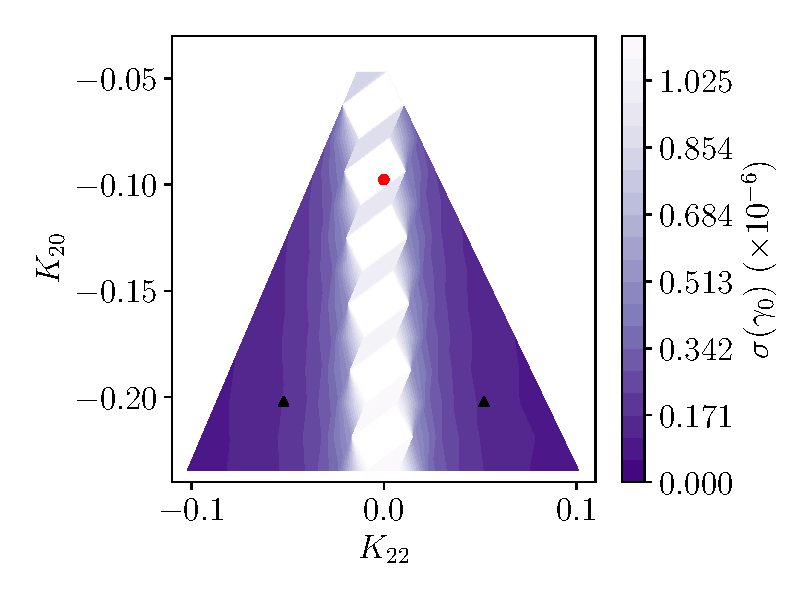
\includegraphics[width=0.33\textwidth]{figs/probe-space-theta-1-sigma.pdf}\hfill
  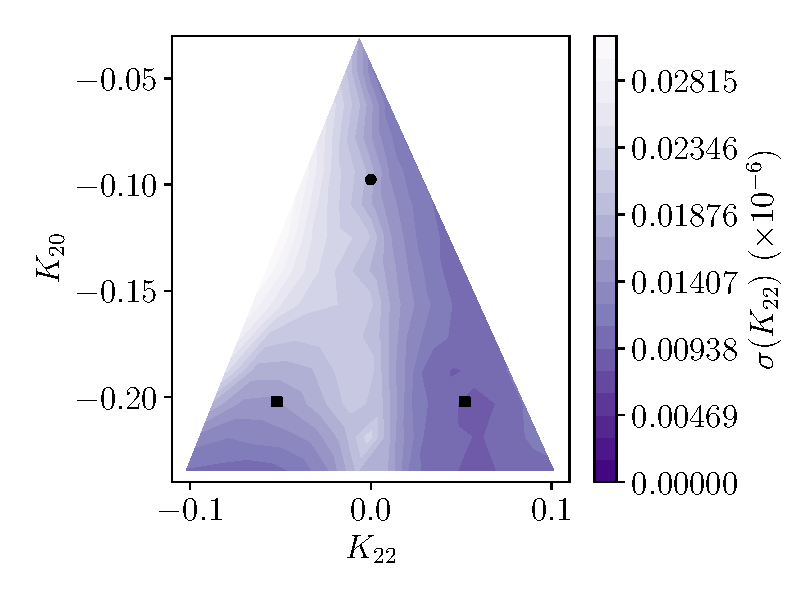
\includegraphics[width=0.33\textwidth]{figs/probe-space-theta-2-sigma.pdf}\hfill
  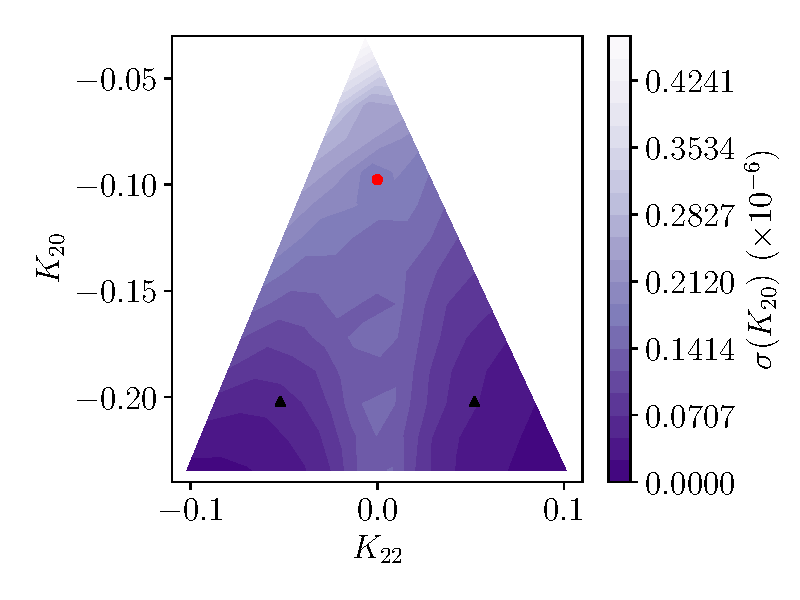
\includegraphics[width=0.33\textwidth]{figs/probe-space-theta-3-sigma.pdf}

  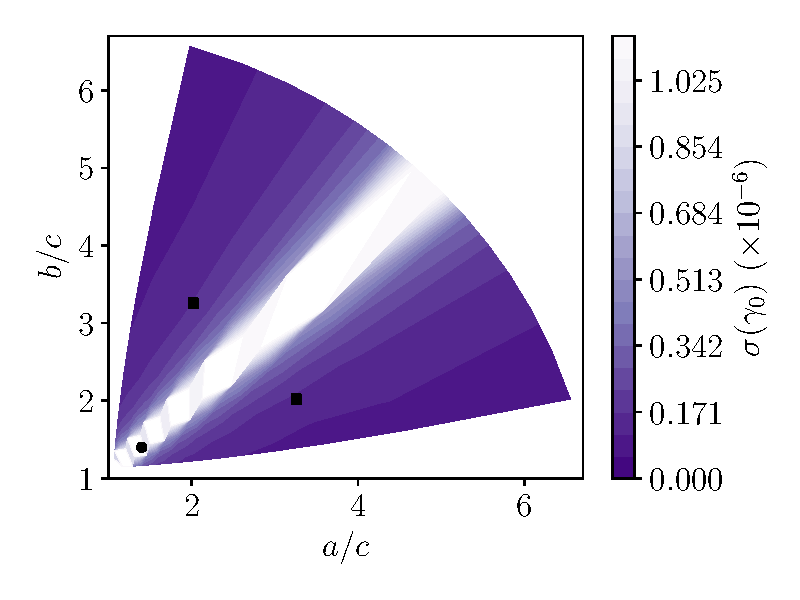
\includegraphics[width=0.33\textwidth]{figs/probe-space-ab-1-sigma.pdf}\hfill
  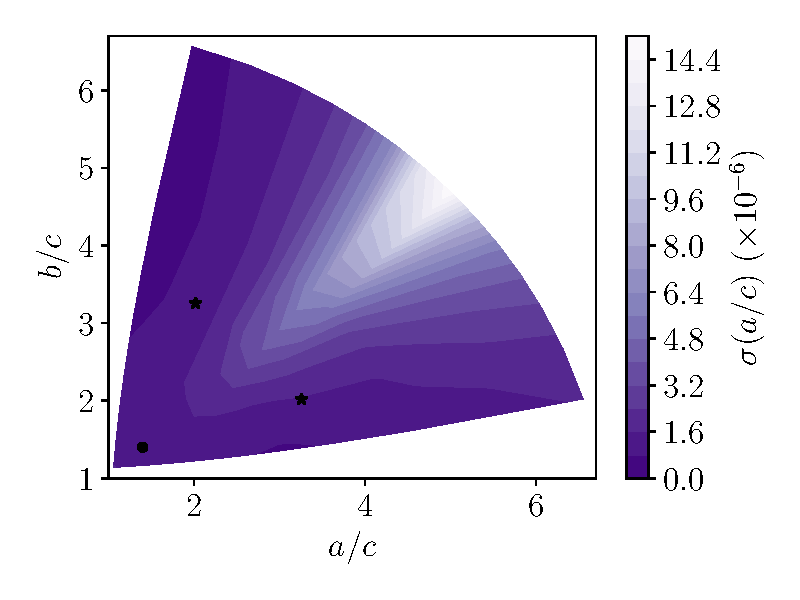
\includegraphics[width=0.33\textwidth]{figs/probe-space-ab-a-sigma.pdf}\hfill
  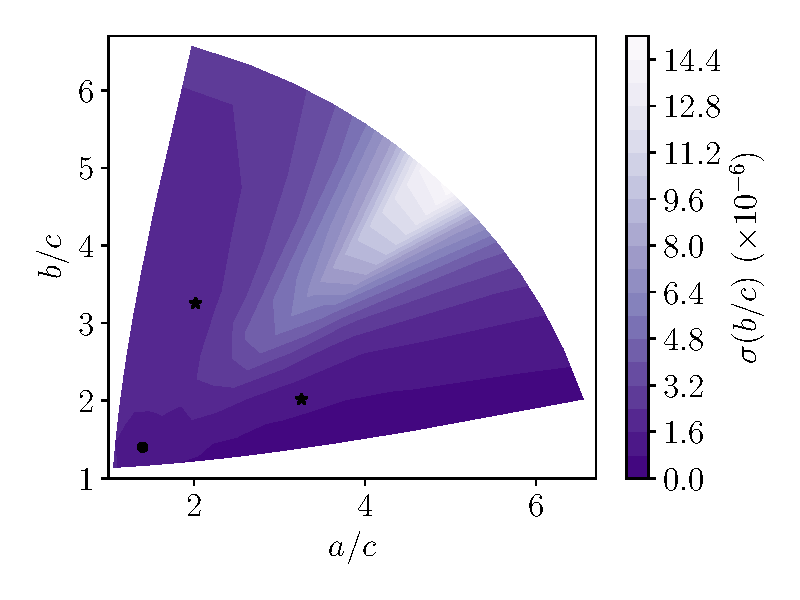
\includegraphics[width=0.33\textwidth]{figs/probe-space-ab-b-sigma.pdf}

  \caption{1$\sigma$ confidence interval for fit parameters $\gamma_0$, $K_{22}$, and $K_{20}$ (\textit{top row}) and $\gamma_0$, $a/c$, and $b/c$ (\textit{bottom row}). Also shown as black points are the reference asteroid shapes; the symmetric case is marked with a red circle and the asymmetric with a black triangle.}
  \label{fig:scan-space-sigma}
\end{figure*}

To remove the inflated uncertainty, one could assume a rotationally symmetric asteroid, remove $\gamma_0$ as a parameter, and run a fit. For a nearly rotationally symmetric asteroid however, a new parametrization is necessary which does not contain the ill-constrained $\gamma_0$ parameter. This task is beyond the scope of this paper, so we mostly consider asymmetric asteroids throughout.

Figure \ref{fig:scan-space-sigma} also shows low uncertainty for highly asymmetric asteroids, where $b/c$ and $a/c$ are very different (i.e., when $|K_{22}|$ is large). Additionally, $\sigma(K_{20})$ and $\sigma(K_{22})$ decrease for large $|K_{20}|$, which corresponds to large axis ratios in the ellipsoid case.

Figure \ref{fig:scan-space-corr} displays the correlation between the first-order parameters for reference. They show that $\gamma_0$ and $K_{22}$ are often correlated for asymmetric asteroids, while $\gamma_0$ and $K_{20}$ are usually not. This is expected as $K_{22}$ is dependent on the orientation of the asteroid and $K_{20}$ is not. They also show that $K_{22}$ and $K_{20}$ are usually correlated, and that $a/c$ and $b/c$ are highly correlated. The latter is expected due to the $1/c$ dependence. As for the former, this correlation could likely be removed by an alternate parametrization, reducing uncertainties in the shape parameters.

\begin{figure*}
  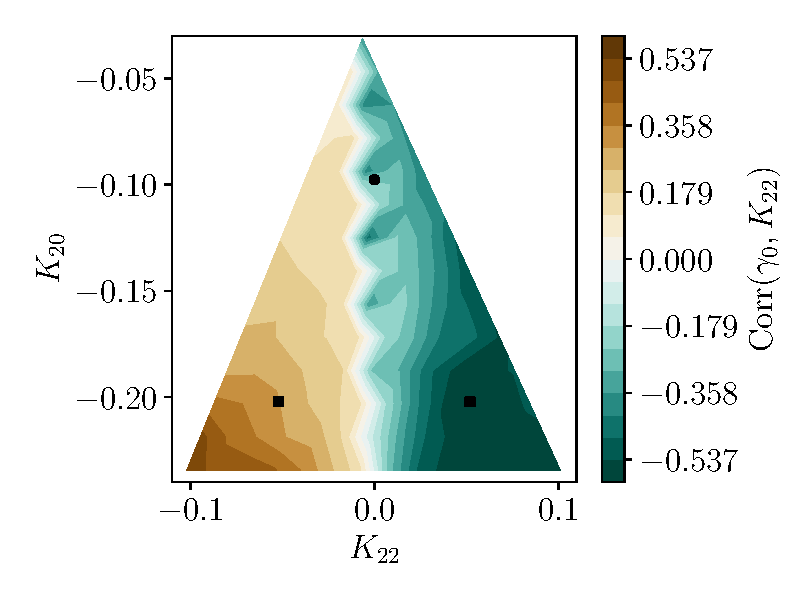
\includegraphics[width=0.33\textwidth]{figs/probe-space-corr12.pdf}\hfill
  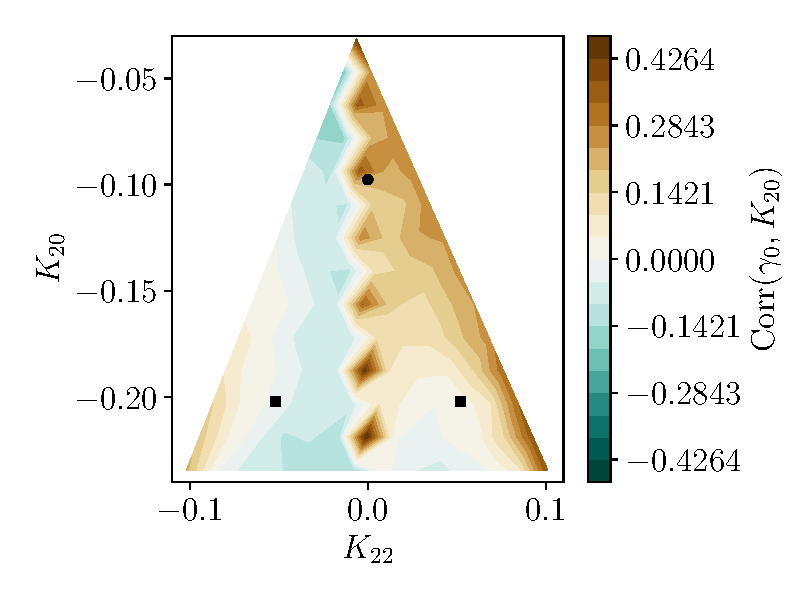
\includegraphics[width=0.33\textwidth]{figs/probe-space-corr13.pdf}\hfill
  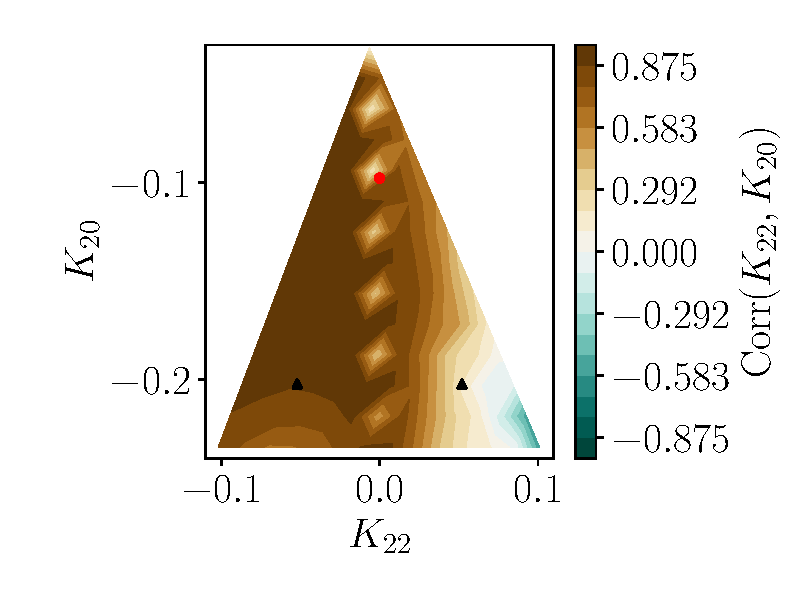
\includegraphics[width=0.33\textwidth]{figs/probe-space-corr23.pdf}

  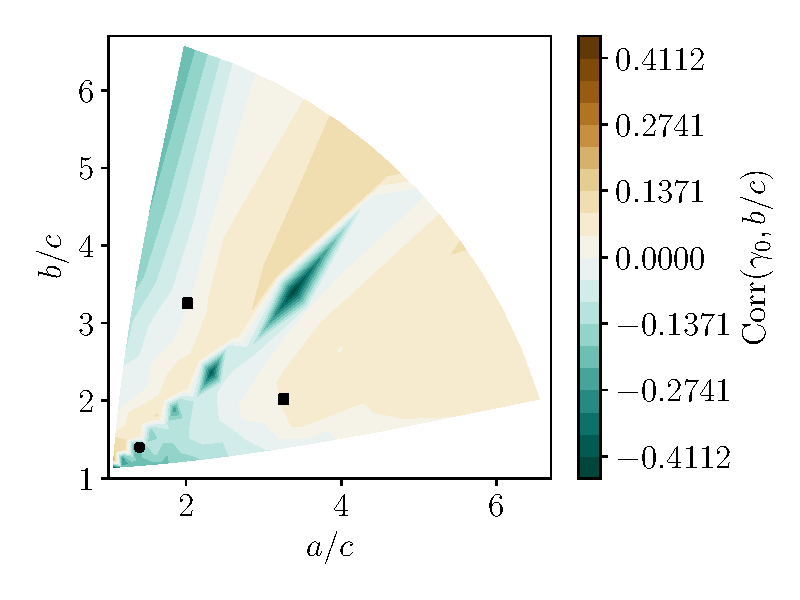
\includegraphics[width=0.33\textwidth]{figs/probe-space-ab-1b.pdf}\hfill
  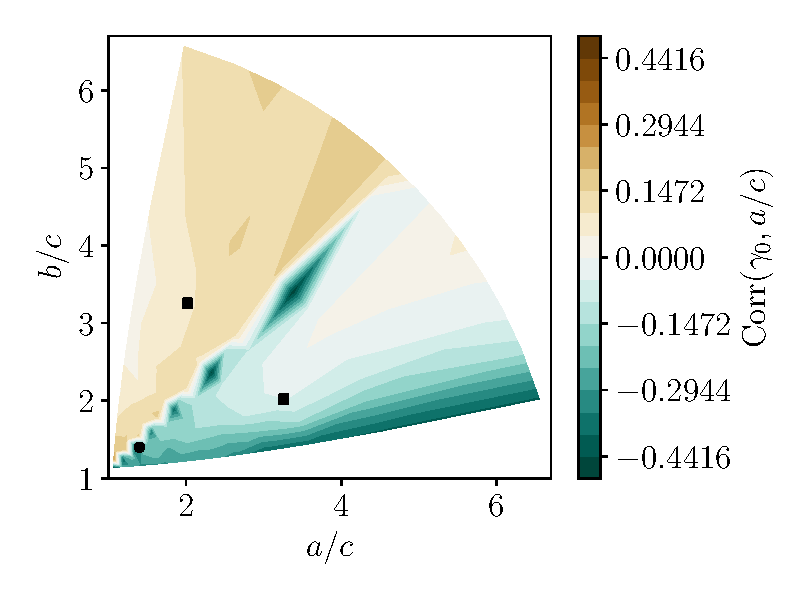
\includegraphics[width=0.33\textwidth]{figs/probe-space-ab-1a.pdf}\hfill
  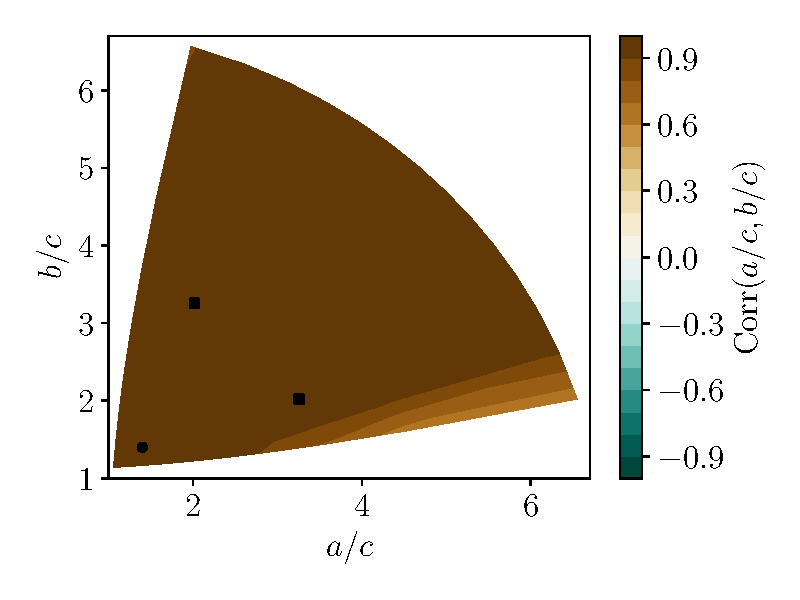
\includegraphics[width=0.33\textwidth]{figs/probe-space-ab-ab.pdf}
  
  \caption{Correlations between PPDs for fit parameters $\gamma_0$, $K_{22}$, and $K_{20}$ (\textit{top row}) and $\gamma_0$, $a/c$, and $b/c$ (\textit{bottom row}).  Also shown as black points are the reference asteroid shapes; the symmetric case is marked with a red circle and the asymmetric with a black triangle.}
  \label{fig:scan-space-corr}
\end{figure*}

Overall, the variation in the uncertainties on $K_{20}$ and $K_{22}$ (the first-order density moments) is present but largely smooth across their allowed parameter space, as is their correlation (except the large $K_{22}$ corner). It therefore seems reasonable to use the asymmetric asteroid shape as a stand-in for an unknown's asteroid shape when simulating an encounter, as we do in this paper. The uncertainty then can be expected to differ across other shapes by a factor of about two or less, as long as the degenerate, symmetric asteroid regime is avoided.

On the other hand, the posterior uncertainty of $K_{3m}$ is much more strongly dependent on asteroid length $a_\mathcal{A}$. Figure \ref{fig:scan-am} displays posterior uncertainty $\sigma$ as a function of $a_\mathcal{A}$, defined in equation \ref{eqn:am}. The vertical axis is shown in log space, meaning that the average of the upper and lower error bars of $\sigma$ is shown instead of showing both as is done in other figures.

\begin{figure}
  \centering
  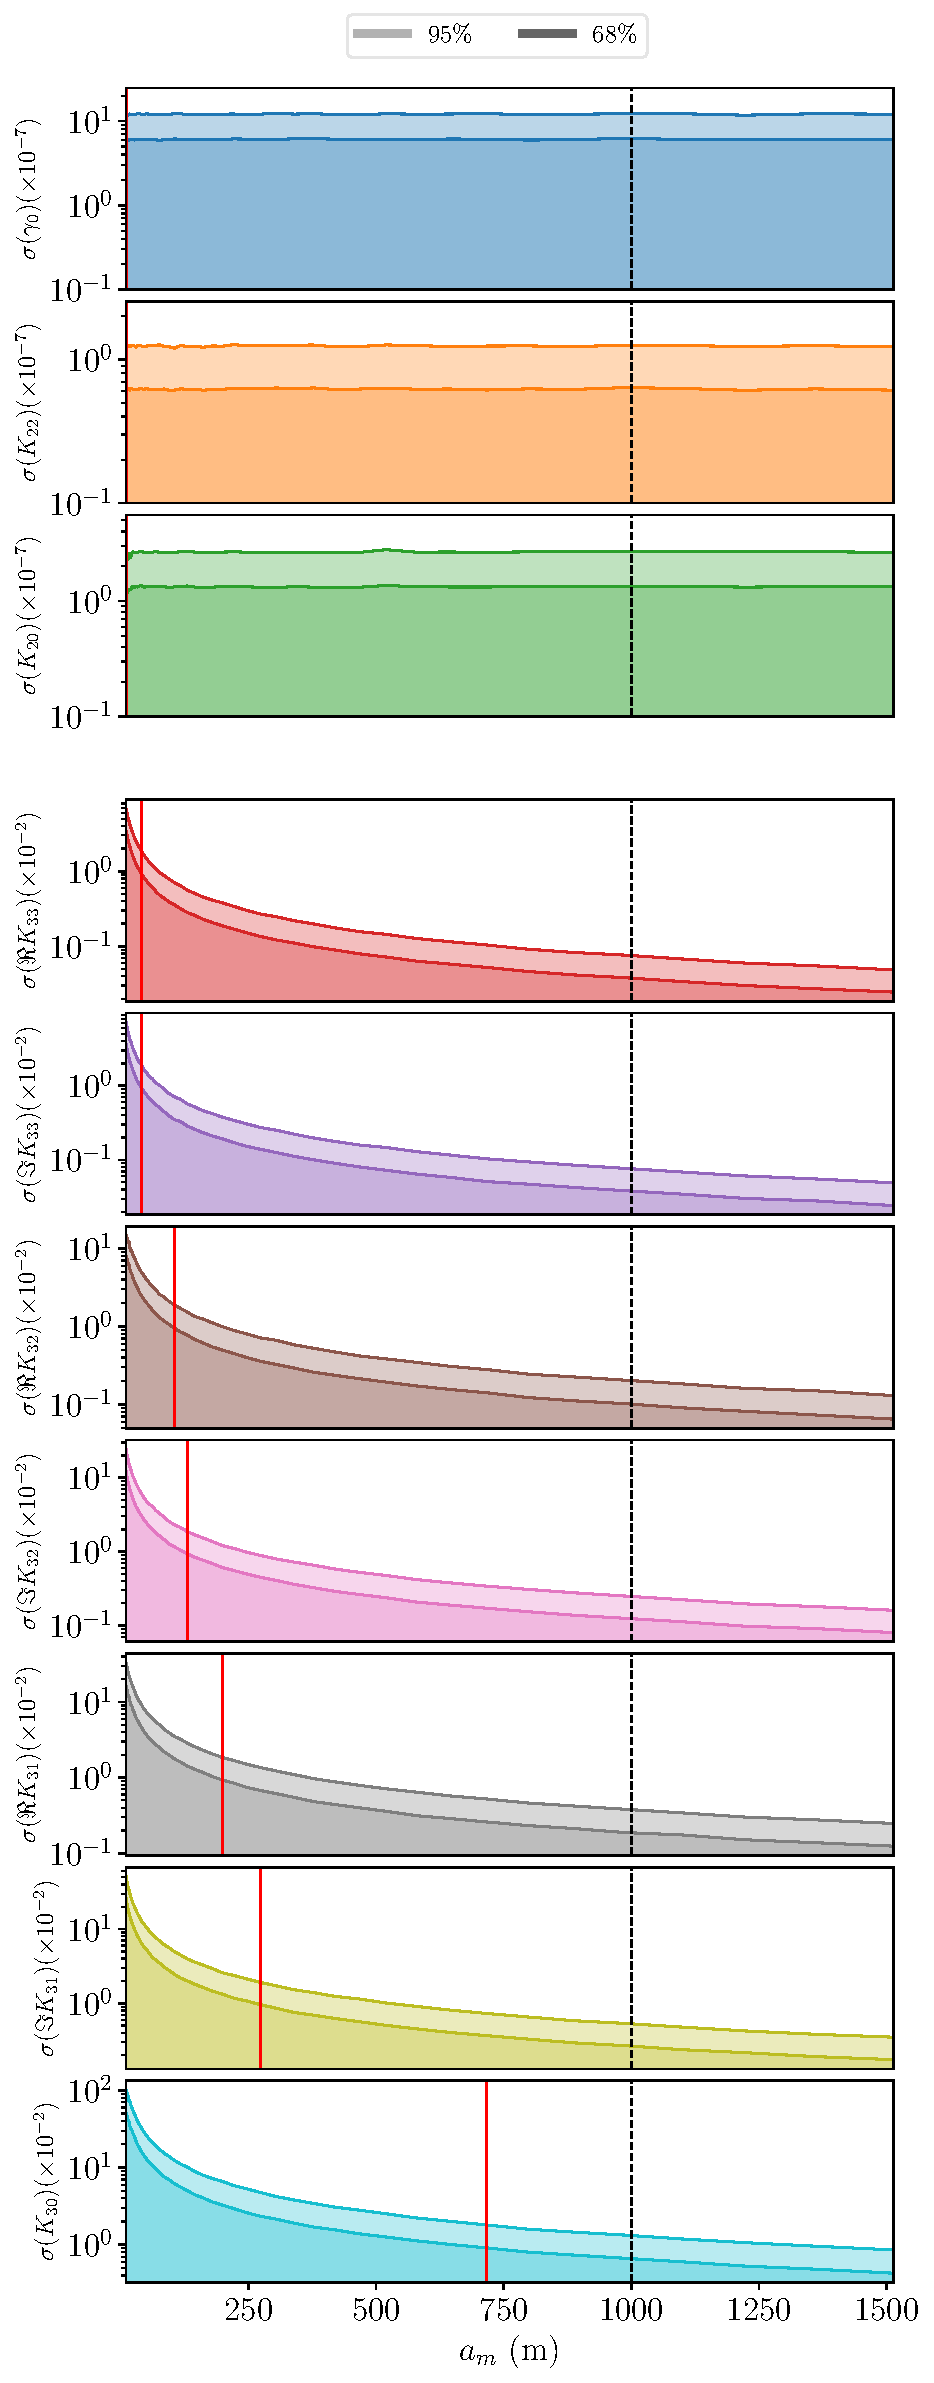
\includegraphics[height=0.89\textheight]{figs/scan-am.pdf}
  \caption{1 and 2$\sigma$ confidence intervals for the first-order parameter PPDs (\textit{top}) and second-order parameters (\textit{bottom}) as a function of asteroid length $a_\mathcal{A}$. The reference cadence is 2 minutes. The red vertical lines indicate when $\sigma = 0.01$. The black dashed line indicates the reference value of $a_\mathcal{A}=1000$ m.}
  \label{fig:scan-am}
\end{figure}

As was mentioned in section \ref{sec:tidal-torque}, the $K_{2m}$ parameters are insensitive to $a_\mathcal{A}$ since the $a_\mathcal{A}^2$ term in $\bm \tau$ (equation \ref{eqn:tidal-torque}) is canceled by the $a_\mathcal{A}^2$ in the moment of inertia (equation \ref{eqn:moi}). The $K_{3m}$ uncertainty is strongly dependent on $a_\mathcal{A}$ for the same reason that uncertainty is strongly dependent on $r_p$: the $(a_\mathcal{A}/D)^{\ell'}$ dependence of equation \ref{eqn:tidal-torque}. At $a_\mathcal{A} \lesssim 700$ m, $K_{30}$ becomes unresolved. The other parameters become unresolved for $a_\mathcal{A} \lesssim 300$ m, with the cut-off for $K_{33}$ being less than 100 meters. This $a_\mathcal{A}$ cut-off is quite sharp; figure \ref{fig:scan-am} shows steep decrease in $\sigma(a_\mathcal{A})$ for low $a_\mathcal{A}$, with an approximate functional form of $\sigma(a_\mathcal{A}) \sim e^{(a_\mathcal{A}/C)^p}$ for a scaling constant $C$ and some power $p < 1$. (In figure \ref{fig:scan-am}, the best fitting values are $p < 0.1$.) This sharpness indicates that the cut-off value of $a_\mathcal{A}$ is unlikely to change significantly if other parameters of the flyby are altered in a way that slightly increases or decreases $\sigma$. It therefore appears that extracting precise $K_{30}$ from asteroids with $a_\mathcal{A} \lesssim 700$ m is very unlikely with this analysis, and for $a_\mathcal{A} \lesssim 50$ m, all $K_{3m}$ will likely be unresolved.

For uniform density asteroids, large $a_\mathcal{A}$ is equivalent to large asteroid radius, which was mentioned in section \ref{sec:moments} and explicitly shown in equation \ref{eqn:ellipsoid-axes}. In non-uniform density asteroids, large $a_\mathcal{A}$ can also be achieved by distributing the mass of the asteroid near the surface, because the $r^2$ term in the integrand of the definition of $a_\mathcal{A}$ causes the density of regions distant from the asteroid centre of mass to dominate $a_\mathcal{A}$.




\subsection{Cadence}
\label{sec:scan-cadence}

The time between observations of asteroid angular velocity, or cadence, may vary depending on the observational schedule of the observing telescopes and the path of the asteroid through the sky.  We measure how the posterior uncertainty $\sigma$ varies with cadence ranging from two minutes to one hour in figure \ref{fig:scan-cadence}.

\begin{figure}
  \centering
  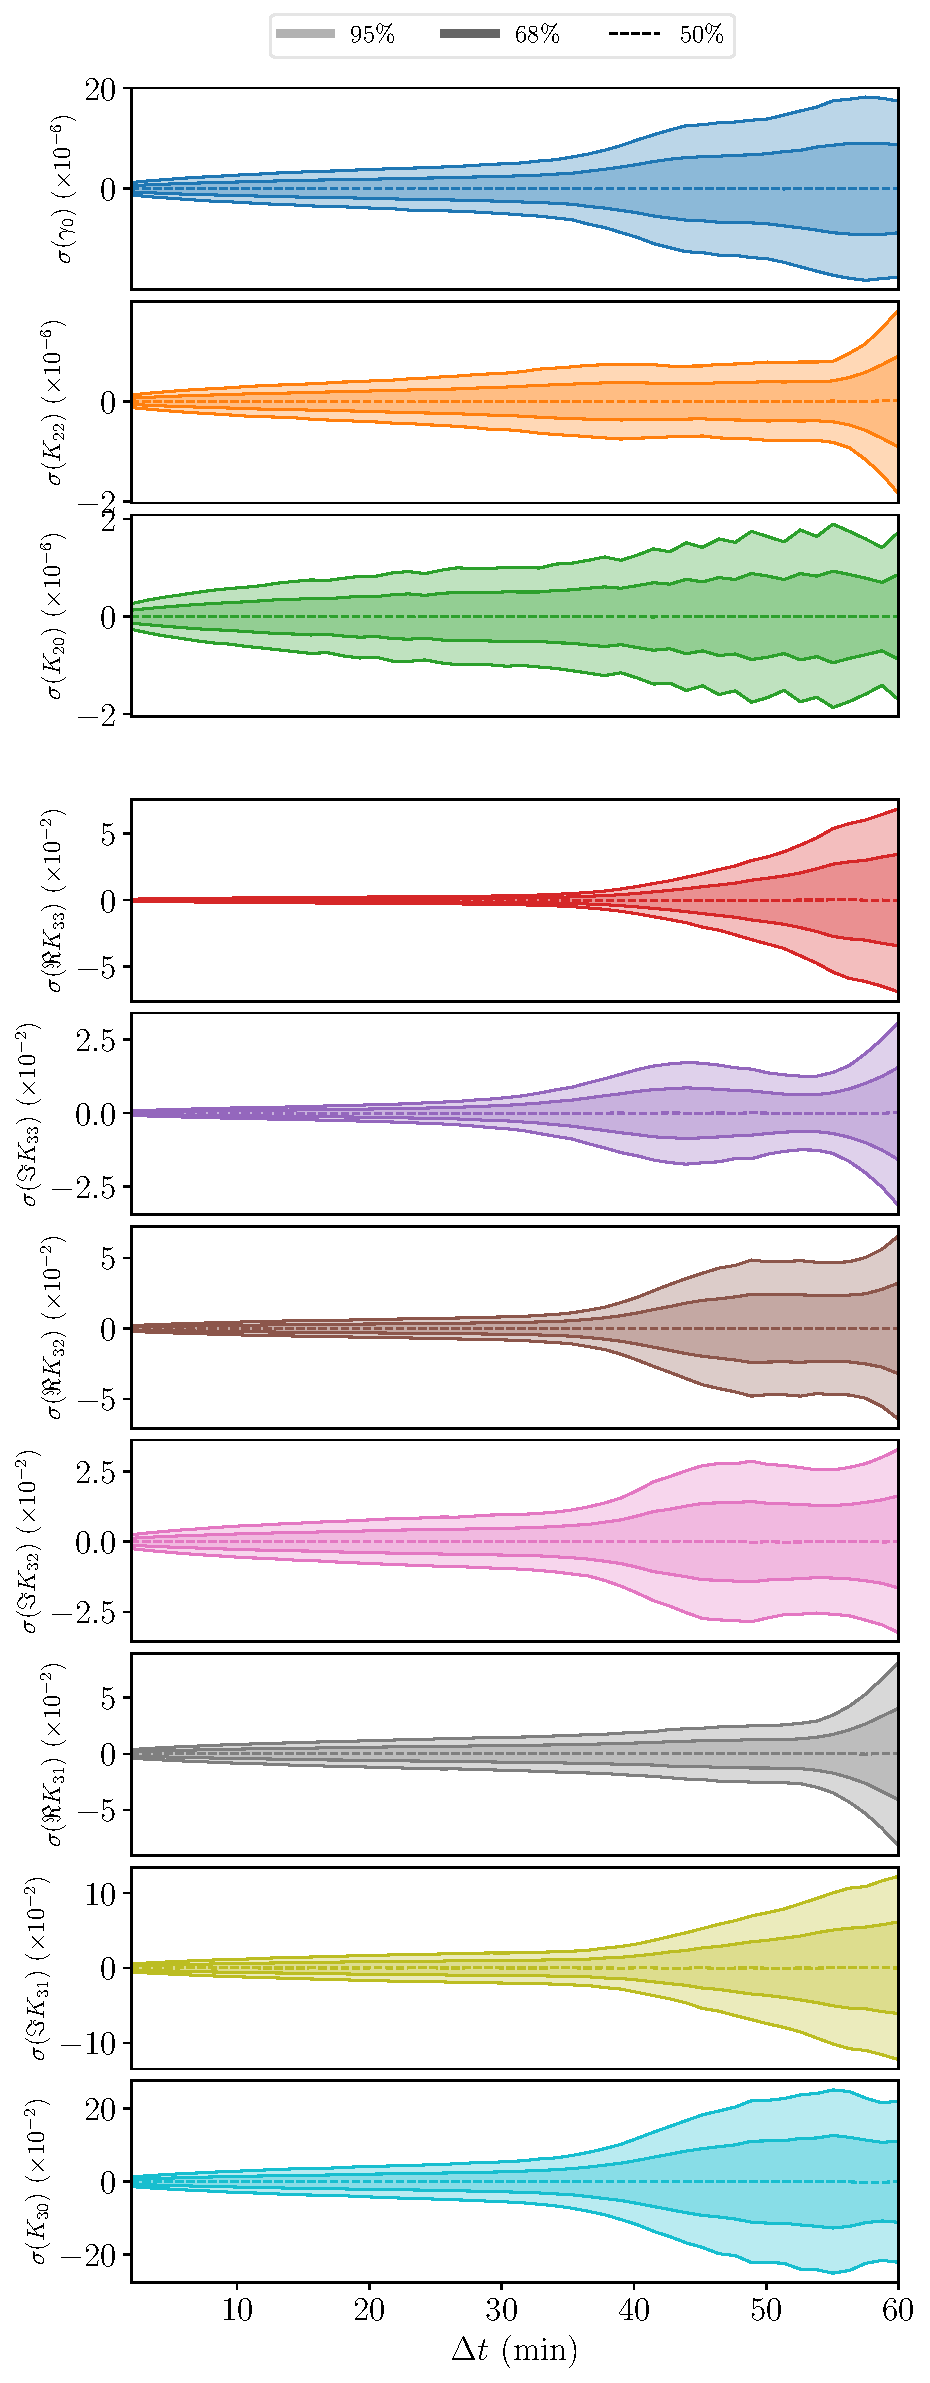
\includegraphics[height=0.89\textheight]{figs/scan-cadence.pdf}
  \caption{1 and 2$\sigma$ confidence intervals for the first-order parameter PPDs (\textit{top}) and second-order parameters (\textit{bottom}) as a function of observational cadence $\Delta t$ The reference cadence is 2 minutes. The red vertical lines indicate when $\sigma = 0.01$.}
  \label{fig:scan-cadence}
\end{figure}

Figure \ref{fig:scan-cadence} displays little dependence of uncertainty on cadence $\Delta t$ for $\Delta t \lesssim 40$ min. We also see flaring of uncertainty for very large cadence, largely driven by the paucity of data points. However, uncertainty dramatically increases for many parameters at about $\Delta t = 30-40$ min, a time scale which is likely characteristic of the asteroid system. We name this rough cadence limit $T_\text{cad}$.

We expect $T_\text{cad}$ to be a function of two dynamical time scales of the system: the rotational period of the asteroid $P_\omega$ and the time spent near perigee $T_p$. The latter can be estimated by
\begin{equation}
  T_p \sim \frac{r_p}{v_\infty}\brackets{2\frac{\mu_\mathcal{B}}{r_pv_\infty^2}+1}^{-\frac{1}{2}}
  \label{eqn:tp}
\end{equation}
which is the ratio of the perigee radius to velocity at perigee. The exact choice of the formula of $T_p$ not obvious, and alternatives to equation \ref{eqn:tp} are possible. For the simulated asteroid, $P_\omega = 9$ hr and $T_p = 42$ min by this definition.

We further study the effect of $P_\omega$ and $T_p$ on $T_\text{cad}$ in appendix \ref{app:cadence-tests}, and find that both affect $T_\text{cad}$ by roughly the same amount.

Figure \ref{fig:scan-cadence} shows that as long as $\Delta t < T_\text{cad}$ is achieved, the influence of cadence on $\sigma$ is minimal (except for $K_{30}$ where the $\sigma<0.01$ limit is slightly exceeded). However, shorter cadence almost always leads to lower uncertainties.



\subsection{Perigee gap}
\label{sec:scan-gap}
In certain circumstances, spin data might not be able to be captured for a close encounter at perigee. The asteroid might dip below the horizon, or it might pass too close to the sun to be observed. Generally, angular velocity data can be collected when the asteroid is distant from the central body, where torque is low. There, the angular velocity evolution is dominated by torque-free precession dictated by the moment of inertia components. That zero-torque data can still be used to fix $K_{20}$ and $K_{22}$ as in \cite{MOSKOVITZ2020113519}. However, $K_{3m}$ are not extractable from precession data alone. We are therefore curious as to how our posterior uncertainties change due to lack of data during the encounter perigee.

To test this, we mask the perigee of the counter by removing a duration $T$ of data centred on the perigee, where $T$ ranges from 0 to 3 hours. To prevent lack of precision on $K_{\ell m}$ induced by lower amounts of data for high $T$, we always cut 3 hr$-T$ from the data set, half from the beginning and half from the end, so that each data set produced for all $T$ has the same length of data before and after the perigee. We then fit the same asteroid model to the cut data for all $T$ and plot posterior uncertainties $\sigma$ in figure \ref{fig:observation-gap}.

\begin{figure}
  \centering
  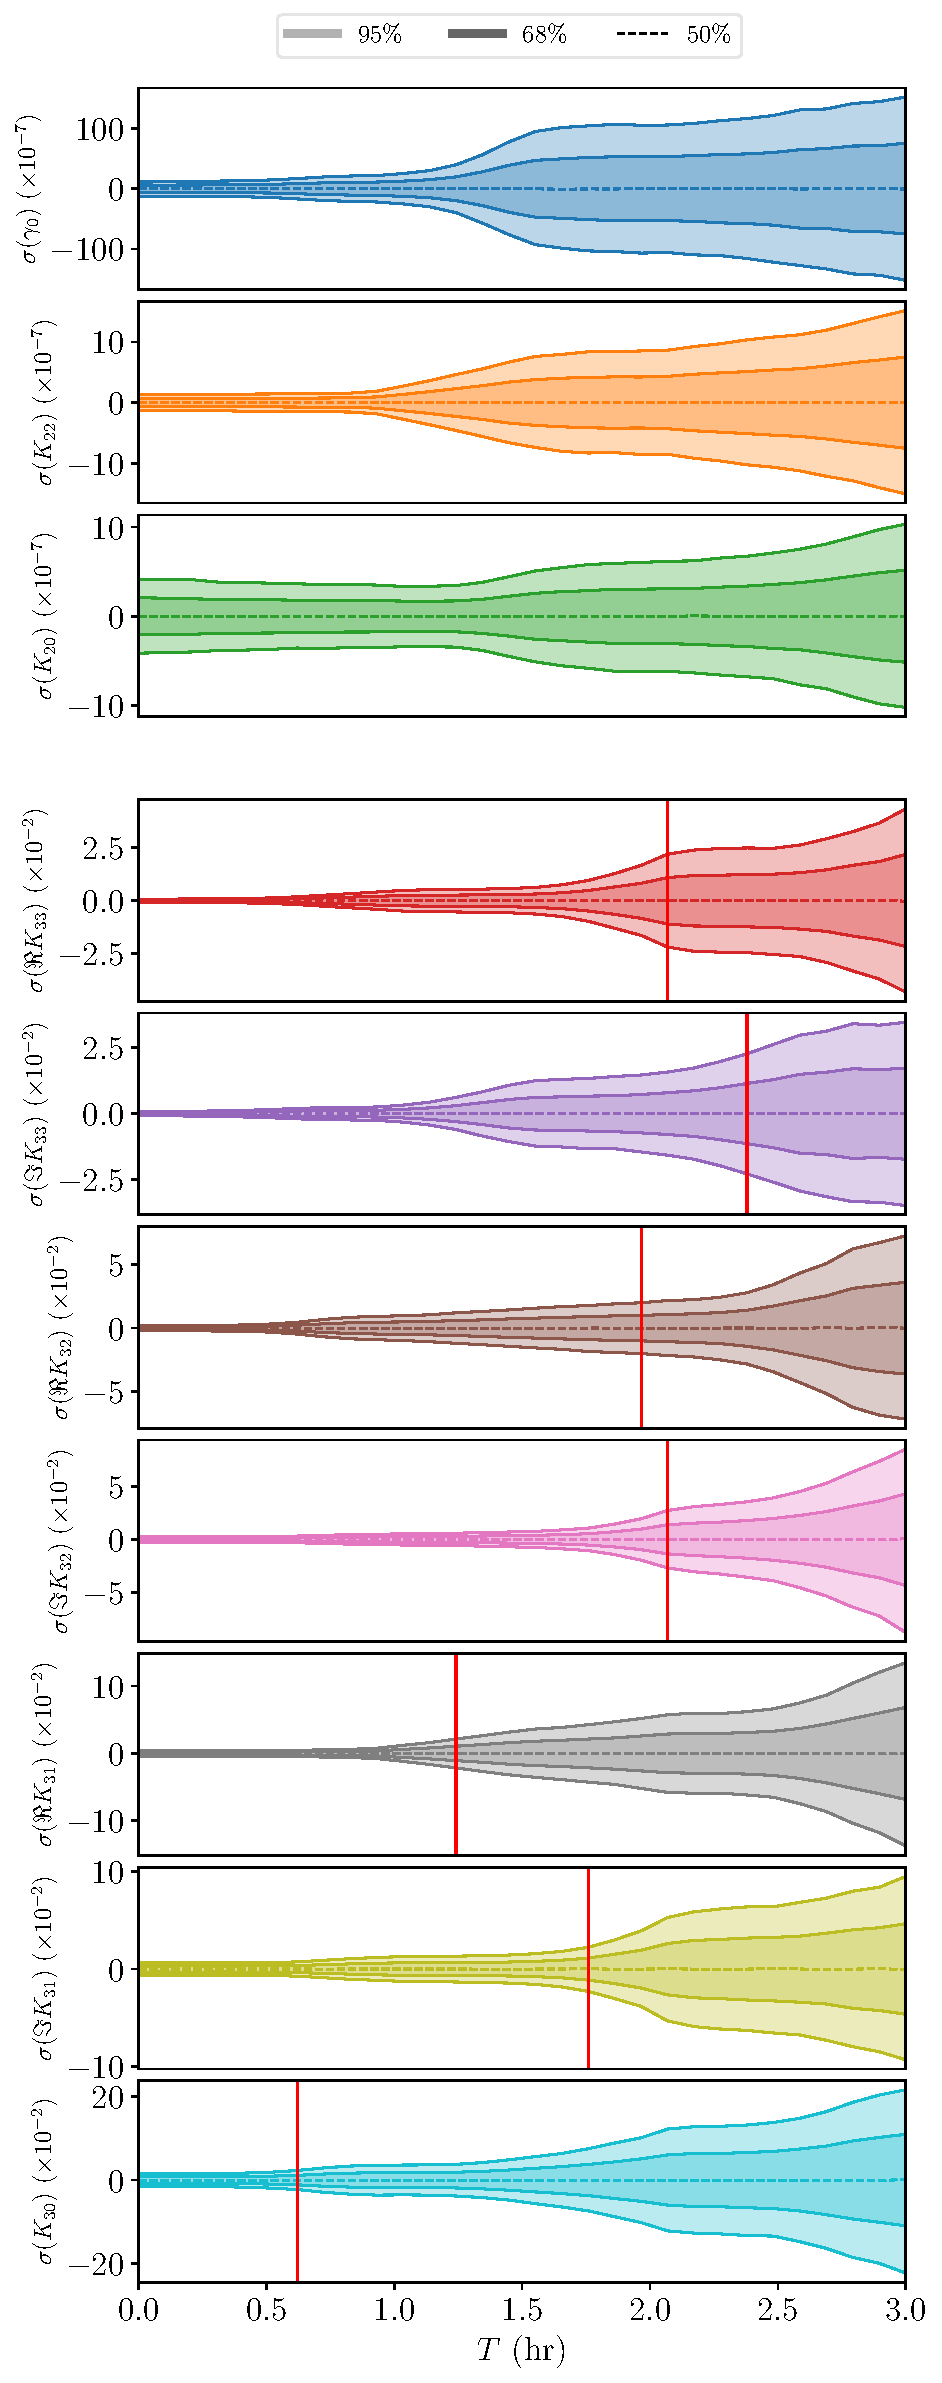
\includegraphics[height=0.89\textheight]{figs/observation-gap.pdf}
  \caption{1 and 2$\sigma$ confidence intervals for the first-order parameter PPDs (\textit{top}) and second-order parameters (\textit{bottom}) as a function of a data gap of width $T$ at perigee. The red vertical lines indicate when $\sigma = 0.01$.}
  \label{fig:observation-gap}
\end{figure}

Since torque is greatest at perigee, we expect that region of the data to contain the most information about $K_{\ell m}$, and therefore uncertainty should increase monotonically with $T$, which is seen in figure \ref{fig:observation-gap}. We also see that the first-order parameters are not as sensitive to $T$ as the second-order parameters, because $K_{2m}$ are additionally constrained by torque-free precession after perigee.

Most parameters show dramatically increased uncertainty in the $T \sim 1-2$ hr range. On the other hand, none of the uncertainties increase noticeably for $T < 30$ min. Thirty minutes of dropped data is equivalent to fifteen dropped points for the simulated cadence of $\Delta t = 2$ minutes, showing that many data points can dropped from the data set at perigee before the uncertainty starts to increase.

Qualitatively, \ref{fig:observation-gap} shows similar dependence of $\sigma$ on $T$ as \ref{fig:scan-cadence} showed for $\sigma$ on cadence $\Delta t$. They also both have cut-offs where uncertainty markedly increases, and both the $T$ and $\Delta t$ cut-offs have qualitatively similar shapes although they occur at different values of $\Delta t$ and $T$. This suggests that the factors that govern uncertainty due to cadence (appendix \ref{app:cadence-tests}) also may govern sensitivity to lack of data at perigee in a similar way.


\subsection{Initial spin pole}
\label{sec:scan-spin}

The tidal torque experienced by the asteroid is affected by the initial direction of asteroid spin $\bm \Omega_0$ both because spin sets the initial asteroid orientation up to $\gamma_0$ and because of the spin-dependence of the rotational equations of motion (equation \ref{eqn:omega-eom}).

In figure \ref{fig:scan-spin}, we display 1$\sigma$ uncertainties for all parameters as a function of the direction of $\bm \Omega_0$, mapped onto the unit sphere in the inertial frame. Our samples for $\bm \Omega_0$ were laid out on a Fibonacci sphere to ensure they were roughly evenly spaced (marked in figure \ref{fig:scan-spin-avg}). To highlight common features across the parameters, we also display the average 1$\sigma$ sensitivity in figure \ref{fig:scan-spin-avg}. The average is weighted such that the uncertainty map for each parameter contributes an equal amount
(the weight of each map is set to one-tenth of the map's mean). This average map is presented in two different projections to allow data at $\unit Z$ to be read.

\begin{figure*}
  \centering
  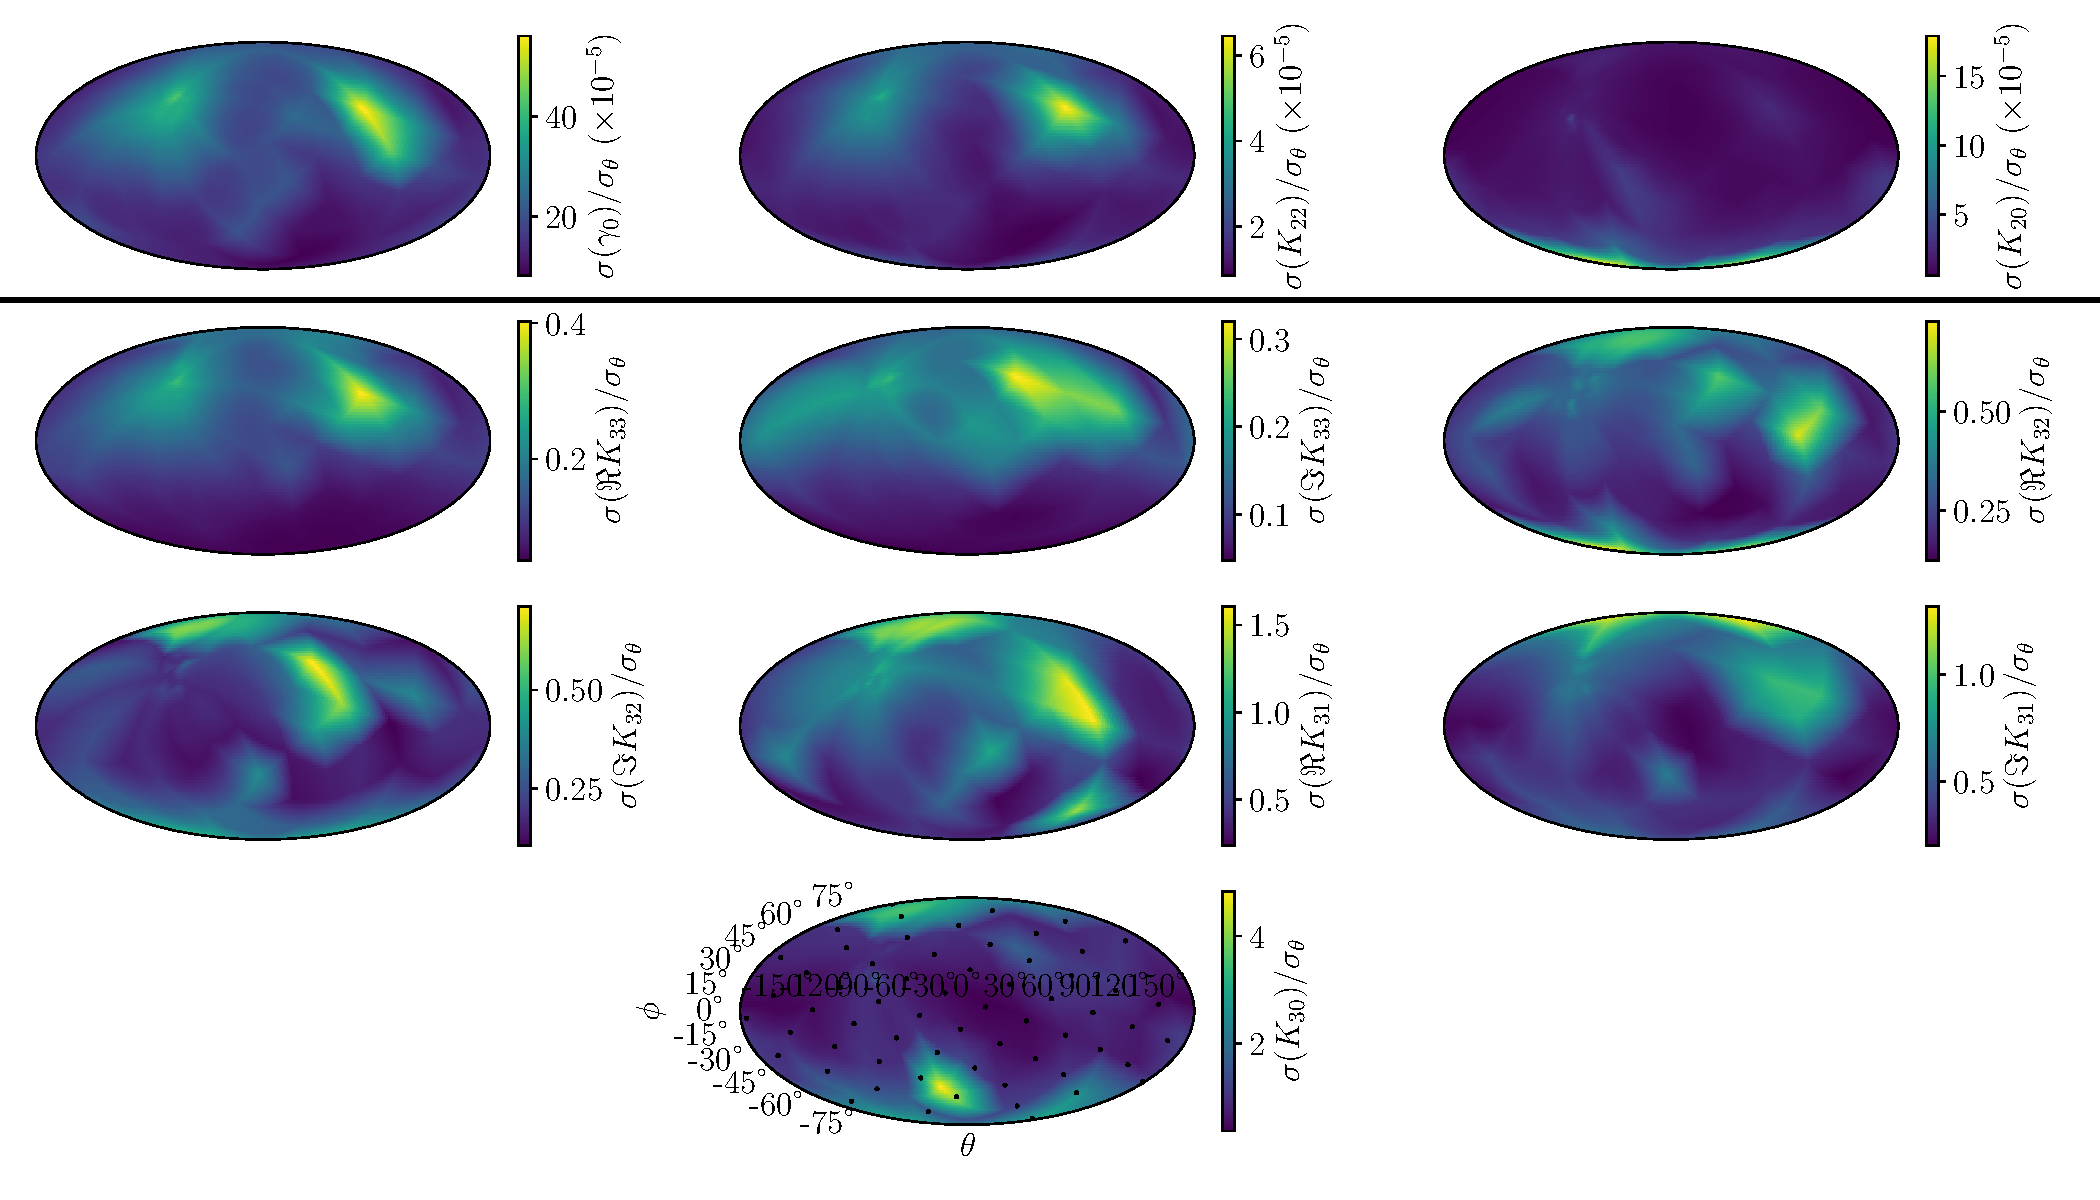
\includegraphics[width=\textwidth]{figs/spin-pole.pdf}
  \caption{$1\sigma$ uncertainties for the first-order parameters (\textit{top}) and second-order (\textit{bottom}) as a function of the initial direction of spin in the inertial frame. All maps are made in the Mollweide projection. The orange star indicates the reference spin pole. The red contours enclose regions where $\sigma \geq 0.01$.}
  \label{fig:scan-spin}
\end{figure*}

\begin{figure*}
  \centering
  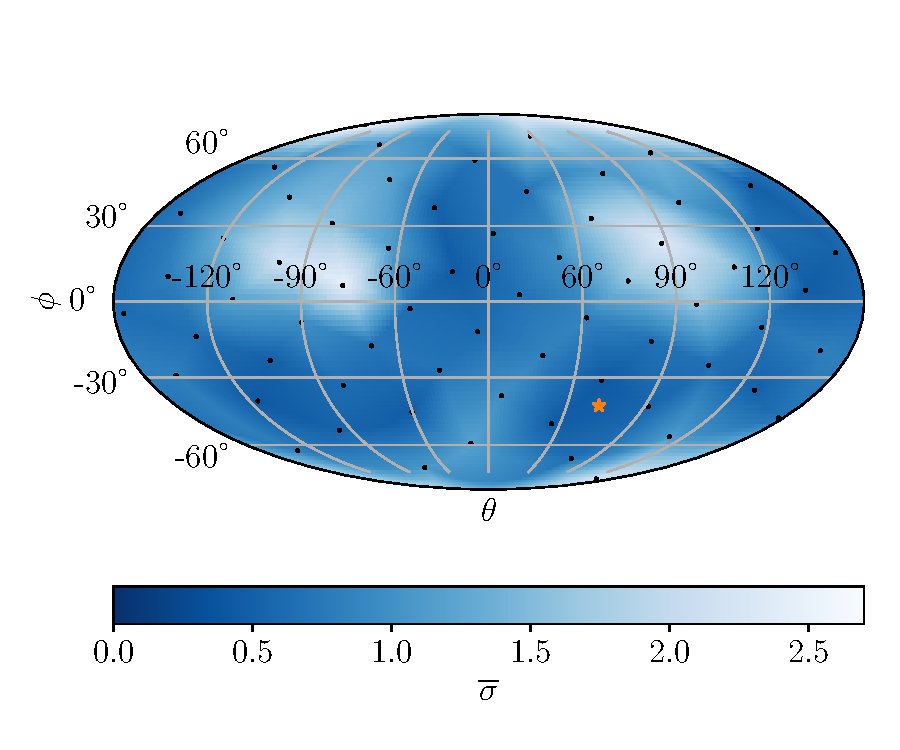
\includegraphics[width=0.45\textwidth]{figs/spin-pole-avg-mollweide.pdf}
  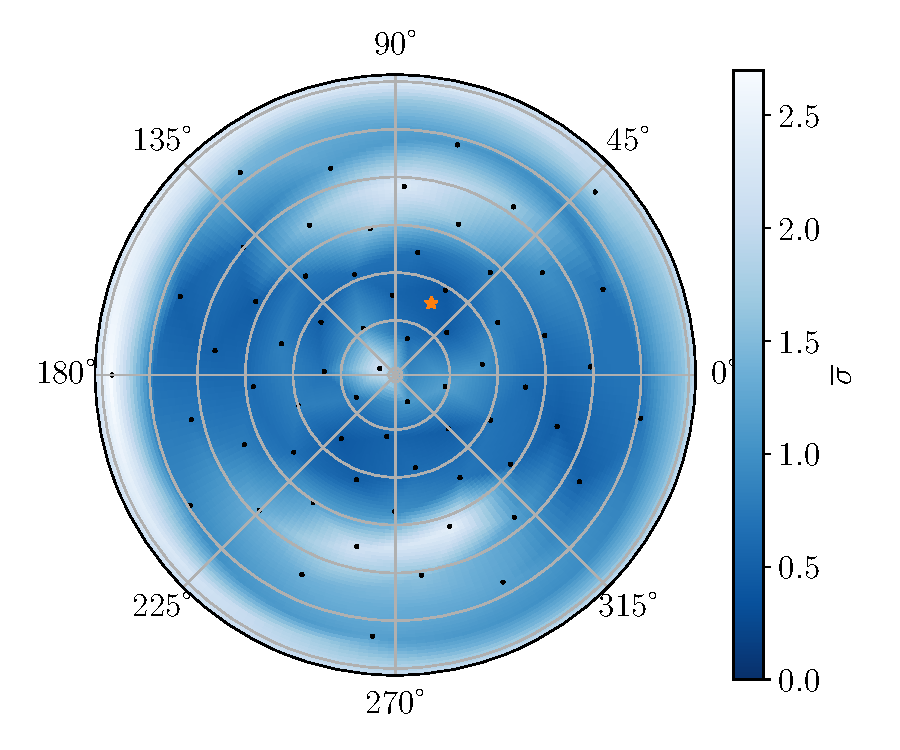
\includegraphics[width=0.45\textwidth]{figs/spin-pole-avg-polar.pdf}
  \caption{The weighted average of the uncertainties shown in figure \ref{fig:scan-spin}, in Mollweide (\textit{left}) and polar (\textit{right}) projections in the inertial frame. See text for a description of how the average was computed. Black dots indicate the Fibonacci-sphere-distributed locations of sample spin poles, and the orange star indicates the reference spin pole. The polar projection is centred at the south pole, or $-\unit Z$.}
  \label{fig:scan-spin-avg}
\end{figure*}

Certain alignments of the body-fixed frame to the inertial frame lead to special conditions on torque, as discussed in section \ref{sec:tidal-torque}. For example, $\bm z \parallel \unit Z$ and $\bm z \parallel \unit Y$ at perigee lead to $\bm \tau \parallel \unit z$ to first-order, and $\bm \tau \parallel \unit X$ at perigee leads to $\bm \tau = 0$ to first-order. We relate this to the initial direction of $\bm \Omega_0$, via the approximation that $\bm \tau$ is small until perigee. Then, since $\bm \omega_0 \parallel \unit z$ in the body-fixed frame as an initial condition (section \ref{sec:sim}), we have that $\bm \Omega_0 \parallel \unit Y$ and $\bm \Omega_0 \parallel \unit Z$ both lead to $\bm \tau \parallel \unit z$, and $\bm \Omega_0 \parallel \unit X$ leads to $\bm \tau = 0$.

Figure \ref{fig:scan-spin-avg} shows area of increased uncertainty for $\bm \Omega_0 \parallel \unit Z$ and $\bm \Omega_0 \parallel \unit Y$, but not the $\unit X$ case. This indicates that $\bm \tau \parallel \unit z$ causes increased uncertainty. Physically, $\bm \tau \parallel \unit z$ only changes an asteroid's rotational period and does not cause it to tumble, eliminating the ability to discern moment of inertia ratios from zero-torque precession after the encounter. Also, $\tau_z$ affected by fewer parameters than $\tau_x$ or $\tau_y$.  Both of these are reasons why $\bm \tau \parallel \unit z$ might inhibit precise fits to spin data. If $\bm \tau = 0$ to first-order, then second-order $\bm \tau$ and non-perigee $\bm \tau$ will dominate, which may increase precision to these usually non-dominant parameters and therefore not have the same increasing effect on $\sigma$.

It is important to note, however, that uncertainty does not vary by much more than a factor of two outside the imprecise regions of $\bm \Omega_0 \parallel \unit Z$ and $\bm \Omega_0 \parallel \unit Y$, though these regions are wide for some parameters. Within the imprecise regions, uncertainty can grow up to four times or more the uncertainty at other $\bm \Omega_0$ values, and can exceed the $\sigma ~0.01$ benchmark. The trends for are roughly consistent across parameters (figure \ref{fig:scan-spin}), leading to clearly visible imprecise regions in the average $\sigma$ (figure \ref{fig:scan-spin-avg}).




\subsection{Rotational period}
\label{sec:scan-period}

We also study the effect of the initial rotational period of the asteroid $P_\omega$ on posterior uncertainty $\sigma$. The dynamical time scales $r_p/v_\infty$ and $\mu_\mathcal{B} / (r_p v_\infty)$ have already been mentioned in the context of the cadence cut-off (section \ref{sec:scan-cadence}), and the ratio between them and $P_\omega$ in principal may affect $\sigma$. In figure \ref{fig:scan-period}, we show $\sigma$ as a function of $P_\omega$ for a range of periods typical of NEOs.

\begin{figure}
  \centering
  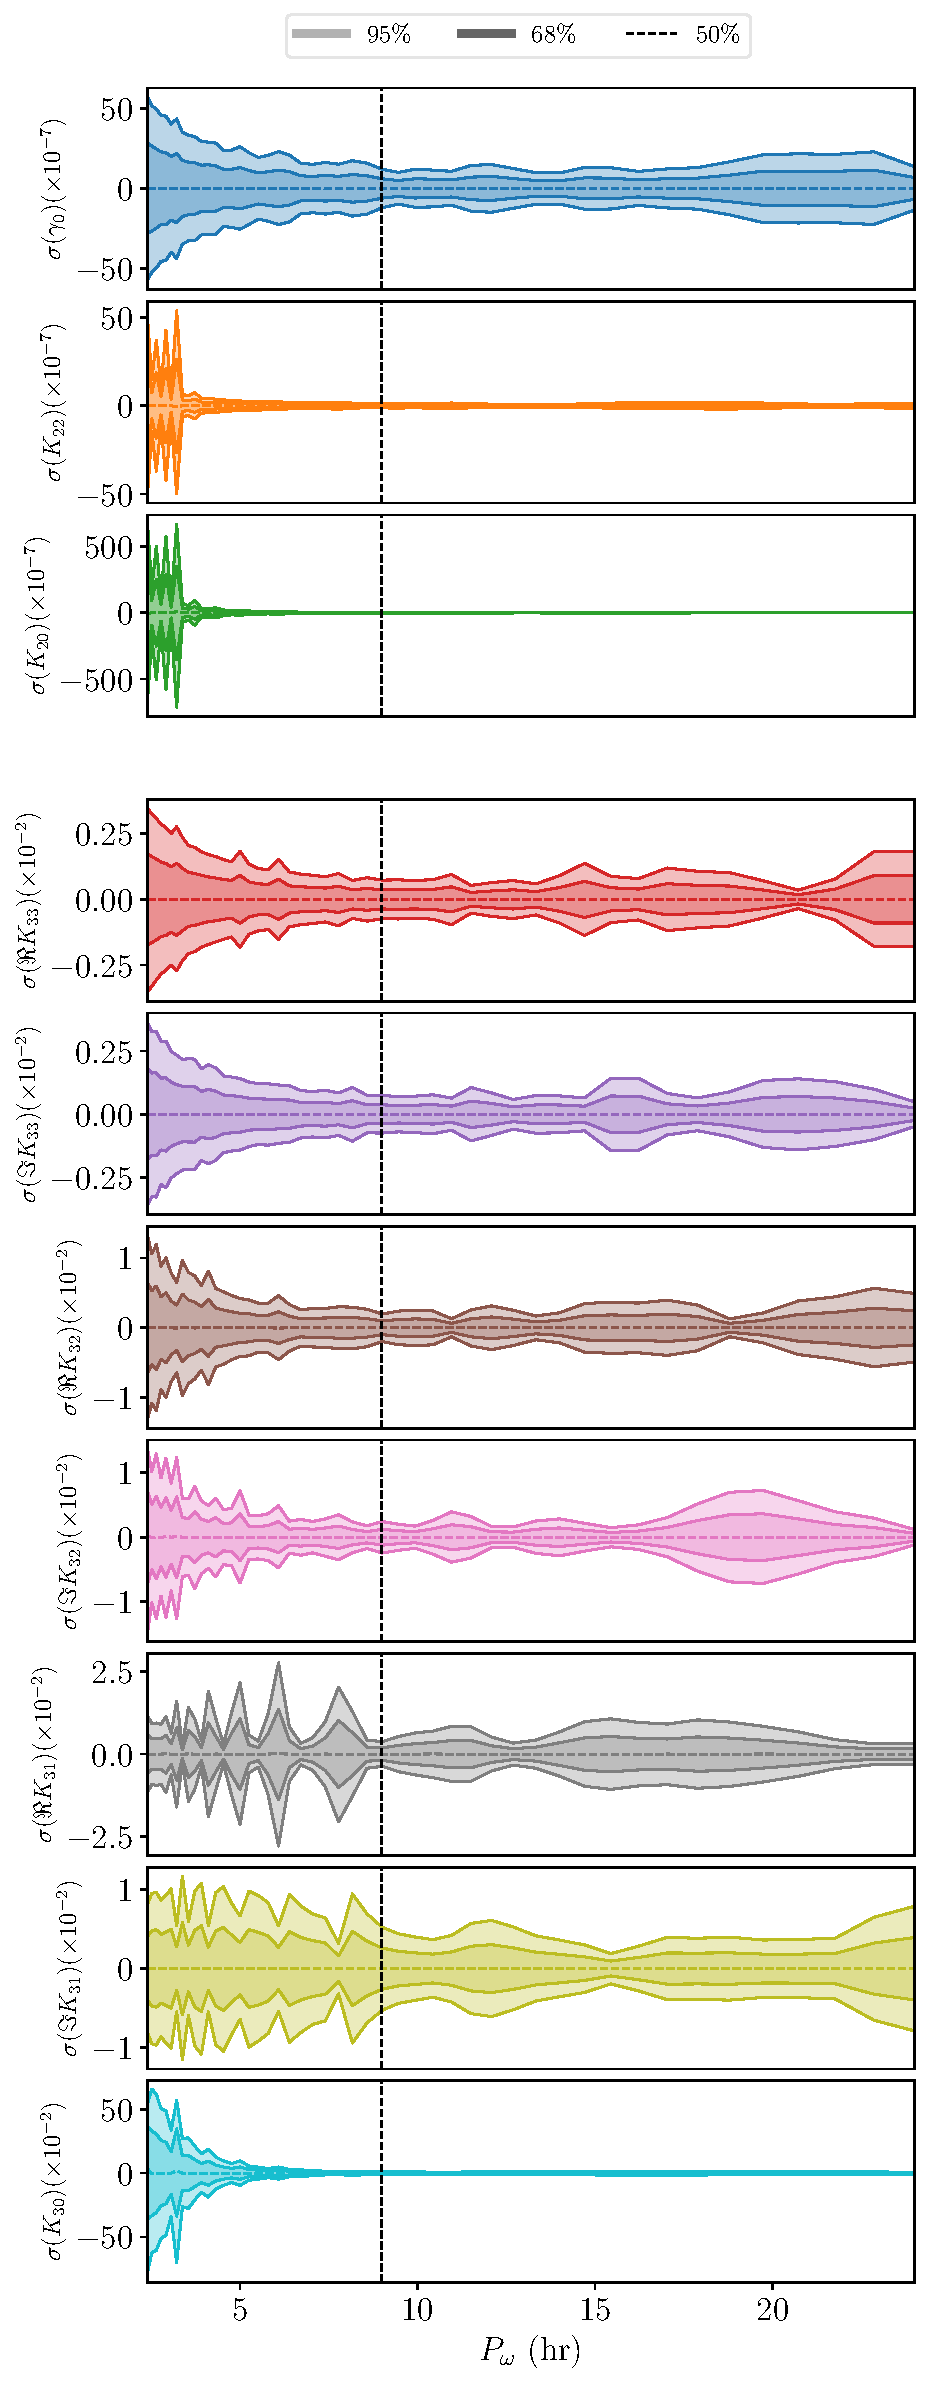
\includegraphics[height=0.89\textheight]{figs/scan-period.pdf}
  \caption{1 and 2$\sigma$ confidence intervals for the first-order parameter PPDs (\textit{top}) and second-order parameters (\textit{bottom}) as a function of initial rotational period $P_\omega$. The reference value of 9 hr is shown as a vertical dotted line. The red vertical lines indicate when $\sigma = 0.01$.}
  \label{fig:scan-period}
\end{figure}

Like figure \ref{fig:scan-vex}, depicting the dependence of $\sigma$ on $v_\infty$, figure \ref{fig:scan-period} shows small-scale variation in uncertainty due to the fact that varying the initial period changes the value of $\gamma$ at perigee, which affects uncertainty to a factor of about two. But a large-scale trend is also visible in many parameters. $K_{20}$ and $K_{22}$ show very large uncertainty for $P_\omega \lesssim 4$ hr because these fast-rotators tumble very little after perigee. This increases uncertainty on the $K_{2m}$ parameters, which are constrained by tumbling.

We expect that quickly rotating asteroids would not tumble because, for small $P_\omega$, the dynamical variables $\bm D$, $\bm \omega$, $\alpha$, and $\beta$ vary much smaller than $\gamma$. Approximating each variable as constant over one full rotation of $\gamma$, we can integrate the first-order contribution of $\bm \tau$ over $\gamma \in (0, 2\pi)$ and reveal that each rotation has zero average first-order torque. Since the first-order torque over each rotational period cancels out, there is no secular torque to force the asteroid to tumble. However, this effect does not apply to the second-order parameters, since the integral over the second-order term of $\bm \tau$ does not vanish, as seen in the figure.

Another feature of figure \ref{fig:scan-period} is that $K_{\ell 0}$ is more uncertain at low $P_\omega$ than the other parameters. This is most visible in the figure for $K_{30}$. The cause is likely that $K_{\ell 0}$ cannot contribute to $\tau_z$ as shown in equation \ref{eqn:tidal-torque}. We already discussed that asteroids with small $P_\omega$ do not tumble, and since $\tau_x$ and $\tau_y$ are what induces tumbling, the most observable component of torque is therefore $\tau_z$, which $K_{\ell 0}$ do not affect.

The most severe effect of period on $\sigma$ is in the low-period regime ($P_\omega \lesssim 5$ hr), but in this case, the most strongly affected parameters are $K_{2m}$, which are generally known better than $K_{3m}$. The effect on the imprecise parameters $K_{3m}$ is small, except for $K_{30}$. It therefore seems as though small-period asteroids are still candidates for observation, although high-period asteroids still have better uncertainty.


\subsection{Central body oblateness}
\label{sec:scan-oblateness}

In all the above studies, we assumed a spherical planet ($J_{\ell m} = 0$ for $\ell \geq 1$). By assumption that $\mu_\mathcal{B} \gg \mu_\mathcal{A}$ (so that the asteroid orbit's focus is the centre of mass of the central body), we have $J_{1m} = 0$. The effect of central body oblateness, then, is limited to the $J_{2m}$ terms, and therefore damped by a factor of $(a_\mathcal{B} / D)^2$. We expect these parameters to have little effect on the asteroid.

Here, we define oblateness as $\epsilon = (I_z - I_x)/(\mu_\mathcal{B} R_M^2)$, where $I_{x,y,z}$ are the central body moments of inertia along the principal axes, and $I_x = I_y$. $R_M$ is the true radius of the body (not $a_\mathcal{B}$ from equation \ref{eqn:jlm}). 

$J_{\ell m}$ is defined in equation \ref{eqn:jlm} with respect to the asteroid orbit, not the principal axes of the central body. However, for an equatorial orbit, the central body principal axes coincide with the asteroid orbit frame and we may express $\epsilon$ simply in terms of $J_{\ell m}$ as $\epsilon = -2J_{20}$ and $J_{22} = 0$. (Some sources such as Ref.~\cite{paterLissauer2015} take $\epsilon=J_{20}$ as their definition of $J_{20}$). For simplicity, we use this equatorial orbit case. If the orbit is non-equatorial, the other $J_{2m}$ terms will be non-zero. Since an oblate ellipsoid is mirror-symmetric around all three axes, table \ref{tab:klm-symmetries} indicates that $J_{3m}$ are all zero. The next order of precision after this oblateness approximation is therefore $J_{4m}$, damped by an additional $(a_\mathcal{B}/D)^2$ factor, and  non-ellipsoid corrections to the central body shape.

Given this conversion between $\epsilon$ and $J_{20}$, we analyze posterior uncertainty $\sigma$ of the first-order parameters as a function of $\epsilon$ across a reasonable range of central body oblatenesses based on those of Solar System planets \cite{paterLissauer2015}. These uncertainties are shown in the top pane of figure \ref{fig:scan-oblateness}, together with linear best-fitting curves for $\sigma(\epsilon)$.

\begin{figure}
  \centering
  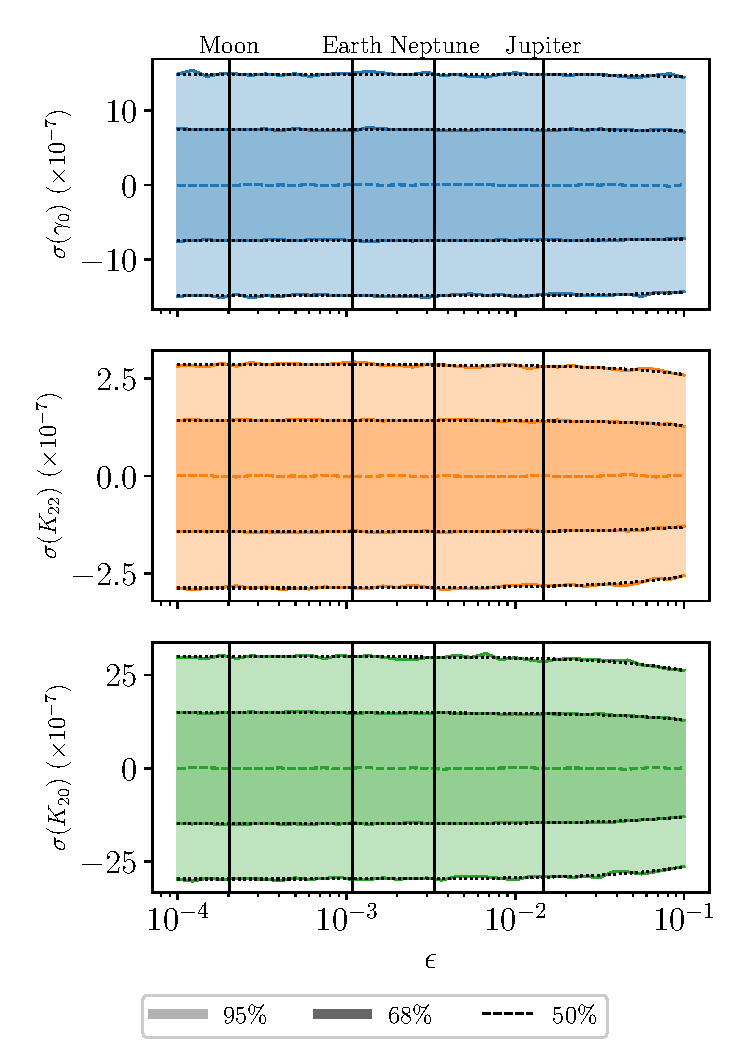
\includegraphics[width=0.88\columnwidth]{figs/oblateness.pdf}
  \vfill
  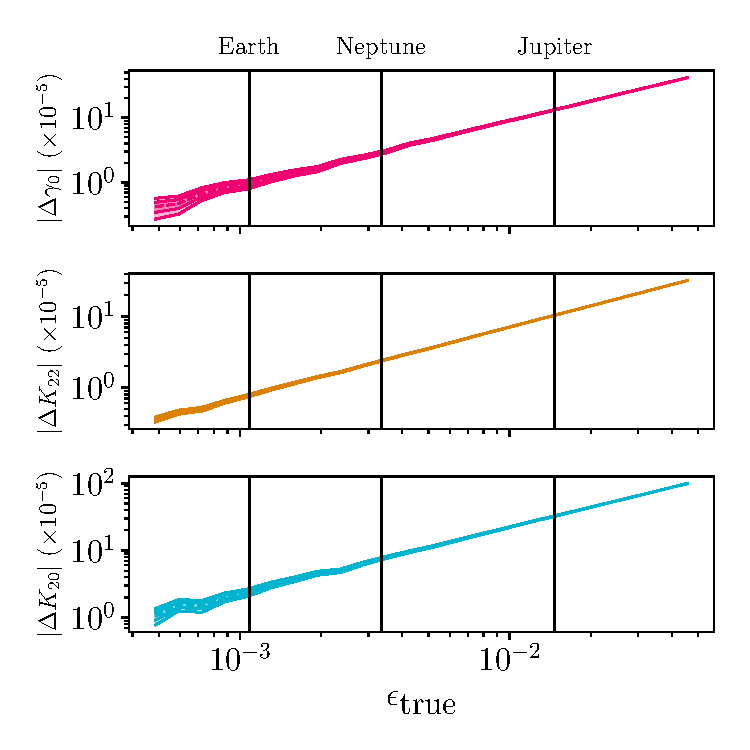
\includegraphics[width=0.88\columnwidth]{figs/oblateness-differ.pdf}
  \caption{\textit{Top}: 1 and 2$\sigma$ confidence intervals for the first-order parameter PPDs as a function of oblateness $\epsilon$ . Linear best-fitting lines to $\sigma$ (black, dotted) are plotted. \textit{Bottom}: The difference between PPD means extracted from a zero-oblateness model and the true parameters given data with true oblateness $\epsilon_\text{true} \neq 0$. Also shown in both figures are the oblatenesses of reference Solar System bodies.}
  \label{fig:scan-oblateness}
\end{figure}

The figure demonstrates a small dependence of $\sigma$ on oblateness $\epsilon$, but the effect is far from important compared to the other factors studied above. Most Solar System bodies do not reach the oblateness necessary to significantly increase precision on the first-order parameters. The best-fitting lines match the uncertainties well, and they have slope of $(\Delta \sigma / \sigma_{\epsilon=0}) / \Delta \epsilon = -0.26$ for $\gamma_0$, $-0.94$ for $K_{22}$, and $-1.2$ for $K_{20}$. The second-order parameters $K_{3m}$ likely depend on oblateness similarly, but fitting these parameters is computationally more expensive and we do not study them here.

Note that if an encounter is executed around one of the non-Earth objects noted in figure \ref{fig:scan-oblateness}, $a_\mathcal{B}$ and $\mu_\mathcal{B}$ will change in addition to $\epsilon$. These two parameters also affect the precision of the fit parameters (appendix \ref{app:jupiter-earth}), so the figure does not show that encounters with other bodies have the same precision as encounters with Earth; only that the difference in oblateness between the two bodies is of little concern.

Given the small effect of $\epsilon$ on $K_{\ell m}$, it might be tempting to neglect the planetary oblateness when fitting $K_{\ell m}$ to data. However, the bottom pane of figure \ref{fig:scan-oblateness} demonstrates that doing so is invalid. This figure displays $K_{\ell m}$ as extracted by a fit assuming $\epsilon = 0$, but run on data generated with non-zero $\epsilon$. The difference between the PPD means and true parameters are shown. Posterior uncertainties are also shown as bands. The figure shows that even for low (Moon-scale) oblateness, the fit results are inconsistent with the true $K_{\ell m}$ values, since $\Delta K_{\ell m} = 0$ is not contained in the 2$\sigma$ band. This effect is much worse for large oblateness, growing to a difference on the order of $10^{-2}$ between the true and fit parameters for large oblateness. Therefore, accurately modelling central-body oblateness to high precision is essential for accurate estimation of fit parameters. For non-equatorial orbits, with $J_{22} \neq 0$, we also expect $J_{22}$ to affect the accuracy of the fit results to a similar degree, with the additional requirement of using the correct asteroid orbital plane.

Note that $J_{20}$, the parameter studied in this section, has a slightly more general definition than oblateness. If the planet has a moon, the integral defining $J_{20}$ (equation \ref{eqn:jlm}) can be extended to include this extra mass. Since $J_{20}$ is a second moment, this effect is magnified for large distances of the mass from the central body centre of mass (though the effect is not quite quadratic because $a_\mathcal{B}$ also increases for large distances, and $J_{20}$ is divided by $a_\mathcal{B}^2$). This process is only valid when the asteroid never passes inside the moon's orbit.

As an order-of-magnitude estimate for this effect, two spherical objects with masses and radii of Earth and the Moon, separated by one Lunar distance, and both lying in the orbital plane has a combined $J_{20} = 0.25$. Extrapolating posterior uncertainty by the slopes of the best fit lines given earlier, this represents a decrease in $\sigma(K_{2m})$ by a factor of about one quarter.

This analysis suggests that large moons such as ours can improve fit quality, but further study of this effect is beyond the scope of this paper. Without a moon to inflate the oblateness of the central body, planetary oblateness does not significantly improve posterior uncertainty. However, correct representation of oblateness is essential to accurately estimate $K_{\ell m}$.



\section{Density distributions}
\label{sec:distros}

Hitherto, we have only discussed the density moments $K_{\ell m}$ of the asteroid rather than the true density distribution $\rho(\bm r)$. This is because only the density moments are observable by tidal torque interactions. However, by making sufficient assumptions about the density distribution, we can nevertheless estimate $\rho(\bm r)$ from $K_{\ell m}$.

In this section, we outline three different assumptions which yield different types of density distributions for the same $K_{\ell m}$. One of them can be chosen, or a fourth created, depending on what features are desired to be represented in the density distribution. All three of these models assume that $a_\mathcal{A}$ and the asteroid shape is known (for example, by light curve or radar data). Uncertainty on this shape estimate is assumed to be small. The models then produce a density distribution $\rho(\bm r)$ with uncertainty from $K_{\ell m}$ propagated to uncertainty in $\rho$.

In section \ref{sec:results}, we were forced to fix $a_\mathcal{A}$ rather than fit for it because $a_\mathcal{A}$ is degenerate with scaling the $K_{3m}$ components. However, $a_\mathcal{A}$ contains information about the density distribution as shown by its definition in equation \ref{eqn:am}. It might therefore be unreasonable to assume that it is exactly determined by light-curve or radar analysis. If $a_\mathcal{A}$ is too uncertain to be used as a known quantity when extracting density distributions from the moments, then the following models are flexible enough that the $a_\mathcal{A}$ constraint can be removed.

Note that, since the overall mass of the asteroid is not observable from tidal torque, we do not expect to measure $\rho$ in an absolute sense. Only the differences in $\rho$ across the body are measurable.

In section \ref{sec:general-density}, we describe the general form our three models must take. Then in sections \ref{sec:likelihood} to \ref{sec:lumpy} we lay out each individually and compare them in section \ref{sec:density-compare}. In appendix \ref{app:find-surface}, we introduce a new model which does not assume that the asteroid shape is known, instead assuming that the density is constant. This allows us to compute the asteroid shape from $K_{\ell m}$.


\subsection{General density model design}
\label{sec:general-density}

To set the shape of the asteroid, we assume that an indicator function $\mathds{1}(\bm r)$ has been determined such that $\mathds{1}(\bm r) = 1$ inside the asteroid and 0 outside, where $\mathds{1}(\bm r)$ is defined in some frame whose orientation with respect to Earth is known. Since the asteroid rotates around its centre of mass during observations, we assume that the location of the centre of mass is also known in this frame, so that we can set it to be the origin.

We define a new coordinate system, the ``hybrid frame,'' which coincides exactly with body-fixed frame at the initial orientation of the asteroid assuming that the fit result for $\gamma_0$ is perfectly accurate. The orientation of the hybrid frame with respect to the inertial frame is therefore exactly known, so that $\mathds{1}$ is also exact in the hybrid frame. The $K_{\ell m}$ components are known in the body-fixed frame which aligns with the hybrid frame up to uncertainty in $\gamma_0$. We will solve for $\rho(\bm r)$ in the hybrid frame given fit results $K_{\ell m}$ (known in the body-fixed frame) and the fixed $a_\mathcal{A}$ (equal in all frames).

The density moments defined in equation \ref{eqn:klm} are not linear in $\rho(\bm r)$, but we may fix $a_\mathcal{A}$ at the value assumed during the fit, removing the non-linearity induced by division by $a_\mathcal{A}$. Furthermore, since the system is independent of the total asteroid mass, we set $\mu_\mathcal{A}$ equal to an arbitrary constant which makes equation \ref{eqn:klm} linear in $\rho(\bm r)$. Similarly, the form of equation \ref{eqn:am} guarantees that $a_\mathcal{A}^2$ is linear in $\rho(\bm r)$. Equation \ref{eqn:am} and the $K_{00}=1$ component of equation \ref{eqn:klm} can each be applied as constraints to enforce these choices of $a_\mathcal{A}^2$ and $\mu_\mathcal{A}$.

Suppose that we restrict the number of degrees of freedom of $\rho(\bm r)$ from infinity to $m$ by explicitly defining some function $\rho(\bm r, \bm \Theta)$ for an $m$-dimensional vector $\bm \Theta$ which contains the free parameters of $\rho$. We will leave the explicit definition of $\rho(\bm r, \bm \Theta)$ to the model descriptions below, but for now we assume that $\rho$ is linear in $\bm \Theta$; i.e.,
\begin{equation}
  \rho(\bm r, \bm \Theta) = \bm B(\bm r) \cdot \bm \Theta
  \label{eqn:density-distro}
\end{equation}
for a $m$-dimensional vector $\bm B(\bm r)$. ($\bm B$ need not be linear in $\bm r$.) Thus, the defining equations of $a_\mathcal{A}^2$ and $K_{\ell m}$ are linear in $\bm \Theta$. We further assume that the model describes a way to reverse this equation, to write
\begin{equation}
  \bm \Theta = A \bm K
  \label{eqn:density-model}
\end{equation}
where $A$ is a matrix. Here, we have arranged $a_\mathcal{A}^2$ and $K_{\ell m}$ into a vector $K$, which we say has $n$ dimensions. The order of this arrangement is irrelevant, as long as it is kept consistent.

To propagate uncertainties from $\bm K$ to $\bm \Theta$ and therefore $\rho(\bm r)$, we need the covariance matrix $\Sigma_K$ for $\bm K$. First, assume that the hybrid frame is offset from the body-fixed frame by some small angle $\Delta \gamma$, which results from uncertainty in $\gamma_0$. Then
\begin{equation}
  K_{\ell m}^\mathrm{hybrid} = e^{-im\Delta \gamma}K_{\ell m}^\mathrm{body-fixed}.
  \label{eqn:body-fixed-to-hybrid}
\end{equation}
by equation \ref{eqn:ylm-rotation}. Since $K_{\ell m}^\mathrm{body-fixed}$ was obtained by an MCMC fit, a large set of PPD-distributed samples is available for $\Delta \gamma$ and $K_{\ell m}^\mathrm{body-fixed}$, and the covariance matrix $\Sigma_K$ can be computed statistically in the hybrid frame by applying equation \ref{eqn:body-fixed-to-hybrid} to the samples. Then, propagation of uncertainty guarantees that the covariance matrix of $\bm \Theta$ is $\Sigma_\Theta = A \Sigma_K A^T$ and the density distribution and uncertainty on density distribution are equal to
\begin{equation}
  \rho(\bm r) = \bm B(\bm r)^T A\bm K \qquad \sigma^2_\rho(\bm r) = \bm B(\bm r)^T A \Sigma_K A^T \bm B(\bm r).
  \label{eqn:unc-rho}
\end{equation}

The purpose of a model is therefore to restrict the space of valid density distributions by defining the $m\times n$-dimensional constant matrix $A$ and the $m$-dimensional vector $\bm B(\bm r)$ such that equations \ref{eqn:density-model} and \ref{eqn:density-distro} are true. Then the density distribution and its uncertainty are given by equation \ref{eqn:unc-rho}.



\subsection{The ``likelihood'' model}
\label{sec:likelihood}

A natural way to restrict the degrees of freedom of $\rho(\bm r)$ is by defining a likelihood function $\mathcal{L}$ on the density distribution and choosing the one distribution which maximizes likelihood and exactly reproduces $\bm K$. We call this method the ``likelihood'' model. This likelihood should not be confused with the likelihood of equation \ref{eqn:log-likelihood}, which was a function of the spin data, not the density distribution. The choice of the density $\mathcal{L}$ is arbitrary, but the linearity of the model design outlined in the previous section will require a Gaussian likelihood.

To employ this likelihood method, we divide the asteroid into a square grid of $m \gg n$ elements, each of which is assumed to have uniform density $\rho_0+\Theta_i$, where $\rho_0$ is constant across the asteroid and $\Theta_i$ is a local deviation. This defines the model function $\bm B(\bm r)$, which is zeroed in all components except for the $i$th, where $i$ is the index of the grid element that contains $\bm r$.

We use a likelihood of 
\begin{equation}
  \mathcal{L}(\bm \Theta) = \prod_{i=1}^m \frac{1}{\sqrt{2\pi \sigma^2}} \exp\parens{-\frac{\Theta_i^2}{2 \sigma^2}}
\end{equation}
with free parameters $\mu$ and $\sigma$. These parameters do not affect the location of the maximum, so we do not define them. Given this likelihood, the log likelihood is proportional to $-|\bm \Theta|^2$. Minimizing the norm of $\bm \Theta$ is therefore equivalent to finding the maximum likelihood.

Putting aside the problem of minimizing the norm, we use the linearity of equations \ref{eqn:klm} and \ref{eqn:am} to write $\bm K = M \bm \Theta$, where the $i$th entry of every row of the $n\times m$ matrix $M$ is the integral presented in equation \ref{eqn:klm} or \ref{eqn:am}, evaluated over the $i$th finite element. We want to solve $\bm K = M \bm \Theta$ for $\bm \Theta$ to match equation \ref{eqn:density-model}, which we do via the Moore-Penrose inverse. Since $m>n$, the Moore-Penrose inverse of $M$ is
\begin{equation}
  A=M^+ = M^*(MM^*)^{-1}
  \label{eqn:mpi-underdetermined}
\end{equation}
where $M^*$ is the adjoint of $M$. The vector $\bm \Theta=M^+\bm K$ is guaranteed to solve $\bm K = M \bm \Theta$, and by the properties of the Moore-Penrose inverse, this $\bm \Theta$ also happens to minimize the norm of all possible $\bm \Theta$ that satisfy the equation. Thus, defining $A=M^+$ also minimizes $\mathcal{L}$ and fully defines the model.

Note that this model is fast to compute; assuming fast matrix multiplication, the matrix inversion of equation \ref{eqn:mpi-underdetermined} is fast because $MM^*$ is an $n$-dimensional square matrix, which is very small compared to the number of finite elements $m$.




\subsection{The ``harmonic'' model}
\label{sec:harmonic}

We now explore a model that seeks to restrict the space of allowed density distributions a different way: we allow only the density distributions with zero Laplacian: $\nabla^2 \rho = 0$ inside the asteroid (the harmonic distributions). We therefore call this model the ``harmonic'' model. The expansion of a harmonic function in spherical coordinates is given by 
\begin{equation}
  \rho(\bm r) = \sum_{\ell m} \Theta_{\ell m}\frac{R_{\ell m}^*(\bm r)}{a_\mathcal{A}^\ell} 
  \label{eqn:harmonic-rho}
\end{equation}
where the terms which lead to $\rho \rightarrow \infty$ at the origin have been removed and $\Theta_{\ell m}$ are free (complex) parameters. Since $\rho$ is real, we have $\Theta_{\ell m}=(-1)^m \Theta_{\ell,-m}^*$. By setting a maximum on $\ell$, we restrict the number of degrees of freedom to $(\ell_\mathrm{max}+ 1)^2$. Choosing the same maximum $\ell$ as the maximum $\ell$ for the $K_{\ell m}$ moments, we have $m=n-1$ coefficients $\Theta_{\ell m}$ which can be stacked into an $m$-dimensional vector $\bm \Theta$.

Inserting equation \ref{eqn:harmonic-rho} into equations \ref{eqn:klm} and \ref{eqn:am}, we get 
\begin{equation}
  K_{\ell' m'} = \sum_{\ell m} \frac{1}{\mu_\mathcal{A} a_\mathcal{A}^{\ell'} a_\mathcal{A}^\ell} \Theta_{\ell m} \int_\mathcal{A} d^3 r R_{\ell m}^*(\bm r) R_{\ell' m'}(\bm r).
  \label{eqn:harmonic-mat}
\end{equation}
This is an over-determined matrix equation $\bm K = M \bm \Theta$, where $M$ is an $n \times m$ matrix. The Moore-Penrose inverse can therefore be used again to find an inverse $A=M^+$ which yields approximately correct $\bm \Theta$ (approximate in that the norm of the error vector between $\bm K$ and $M \bm \Theta$ is minimized). However, the form of the inverse changes due to the equation being overdetermined:
\begin{equation}
  A=M^+ = (M^*M)^{-1} M^*
  \label{eqn:mpi-overdetermined}
\end{equation}

In the special case where the asteroid is a sphere of radius $R$, the matrix defined by equation \ref{eqn:harmonic-mat} is diagonal, with entries 
\begin{equation}
  M_{\ell m; \ell' m'} = \frac{4\pi R^3}{\mu_\mathcal{A}} \frac{R^{2\ell}}{a_\mathcal{A}^{2\ell}} \frac{\delta_{\ell \ell'} \delta_{m m'}}{(4\ell^2 + 8\ell + 3)(\ell - m)!(\ell+m)!}.
\end{equation}
A non-spherical perturbation will introduce small off-diagonal entries to $M$. This diagonal represents another interpretation of the physical meaning of $K_{\ell m}$; they are directly proportional through this form of $M$ and the matrix equation $\bm K = M \bm \Theta$ to the coefficients of the spherical harmonic expansion of the asteroid density in the case of a spherical asteroid.



\subsection{The ``lumpy'' model}
\label{sec:lumpy}

The above two simple models produce smooth density distributions that generally extend non-uniformity over large regions. In this section, we define a more complicated model which identifies discrete regions differing from the overall density of the asteroid to best fit the measured density moments. We call this model the ``lumpy'' model.

Suppose the asteroid contains $N$ ``lumps'' of uniform mass $\mu_i$ displaced by distance $\bm x_i$ from the asteroid centre of mass and superimposed on a constant-density overall asteroid shape which is known in the form of $\mathds{1}(\bm r)$. For simplicity, we assume that all $N$ regions are ellipsoids with $d$ independent axis lengths. For example, $d=3$ corresponds to an asymmetric ellipsoid, $d=2$ corresponds to a symmetric ellipsoid, and $d=1$ corresponds to a sphere. Recall that $\mathds{1}(\bm r)$ is known in the hybrid frame where the origin is the centre of mass of the asteroid. The displacement of the shape centroid from the centre of mass, which is the opposite of the net displacement of the discrete regions, is therefore observable from light curve analysis. The model therefore has $3(N-1)$ positional degrees of freedom, along with $N$ degrees of freedom for $\mu_i$, $Nd$ shape degrees of freedom, and 0, $2N$, or $3N$ rotational degrees of freedom for $d=1$, 2, or 3 respectively. The sum of these degrees of freedom are displayed in table \ref{tab:lump-dof}. These degrees of freedom should be compared to the known density moments and $a_\mathcal{A}$, of which there are $(\ell_\text{max}+1)^2+1$. However, three of these are the centre of mass of the asteroid which is guaranteed to be correct, and one is the unconstrained total mass so the total number of known parameters is $(\ell_\text{max}+1)^2 - 3$, which is 13 when the second-order density moments are known and six when only $K_{2m}$ are known. We assume that the degrees of freedom of this lumpy model are always fewer than the number of $\bm K$ known, so that the model is overdetermined.

\begin{table}
  \centering
  \begin{tabular}{cc|ccc}
    \hline \hline
        &  & & $N$ &  \\
        &  & 1  & 2  & 3  \\ \hline 
        & 1& \cellcolor{black}\color{white} 2 & \cellcolor{gray}\color{white} 7 & \cellcolor{gray}\color{white} 12\\
    $d$ & 2& \cellcolor{black}\color{white} 5 & \cellcolor{gray}\color{white} 13 & 21 \\
        & 3& \cellcolor{gray}\color{white}  7 &  17 &  27 \\
    \hline \hline
  \end{tabular}
  \caption{Total degrees of freedom $D$ as a function of $N$, the number of lumps modelled, and $d$, the number of independent axis lengths considered for each lump. The configurations with $D \leq$ the six known parameters not including $K_{3m}$ are coloured black, and with $D \leq$ the 13 parameters including $K_{3m}$ parameters are coloured gray.}
  \label{tab:lump-dof}
\end{table}

The net $K_{\ell m}$ components of such an ensemble obey
\begin{equation}
  K_{\ell m} = K_{\ell m}'^0 + \sum_{i=1}^N K_{\ell m}'^i \qquad a_\mathcal{A}^2 = a_0'^2 + \sum_{i=1}^N a_i'^2
  \label{eqn:klm-stack}
\end{equation}
where $K_{\ell m}^i$ and $a_i^2$ obey the same definition as $K_{\ell m}$ in equation \ref{eqn:klm} and $a_\mathcal{A}$ in equation \ref{eqn:am} respectively, but integrated over the $i$th lump. Crucially, note that we set normalizing factors $1/(\mu_\mathcal{A} a_\mathcal{A}^\ell)$ and $1/\mu_\mathcal{A}$ in equations \ref{eqn:klm} and \ref{eqn:am} equal to the values for the entire asteroid, not their counterparts for each lump. The zero-indexed parameters indicate the moments of the uniform-density asteroid medium surrounding the lumps. The prime in equation \ref{eqn:klm-stack} denotes that the moments are calculated in the hybrid frame, with its origin at the asteroid centre of mass.

We can relate the primed moments to the moments calculated relative to each lump's centre of mass via the translation rules for solid spherical harmonics:
\begin{equation}
  \begin{split}
  & K_{\ell m}'^i = \sum_{\ell' m'} (-1)^{\ell - \ell'} R_{\ell - \ell', m - m'}(\bm x_i) K_{\ell' m'}^i\\
  & a_i'^2 = a_i^2 + x_i^2 \frac{\mu_i}{\mu_\mathcal{A}}
  \end{split}
  \label{eqn:translate-klm}
\end{equation}
from Ref.~\cite{Gelderen1998TheSO}. The dummy indices $\ell', m'$ should only be summed over values in which $\ell-\ell' \geq 0$ and $|m-m'| \leq \ell - \ell'$. Here, $\mu_i$ is the added mass of lump $i$, while $K_{1m}=0$ and $K_{2m}$ incorporate the lump's orientation and moment of inertia ratios. Its volume is constrained by $a_i^2$. These values map directly onto an ellipsoid shape via equations \ref{eqn:ellipsoid-axes}, so that if $K_{\ell m}^i$, $a_i^2$, $\mu_i$, and $x_i$ are known, then the density distribution of the asteroid is known.

Note that if $\bm x_i$ is known, then equation \ref{eqn:translate-klm} are linear in $K_{\ell m}^i$ and $a_i^2$. Therefore, if we define $\bm \Theta$ to contain $K_{2m}^i$ and $a_i^2$ for all $i$ in some order, then equations \ref{eqn:translate-klm} and \ref{eqn:klm-stack} define a matrix equation $\bm K = \bm C + M \bm \Theta$ which can be solved by setting $A$ equal to the Moore-Penrose inverse of $M$ (equation \ref{eqn:mpi-overdetermined}, since $\bm \Theta$ is overdetermined). Note that the $\bm C$ term of this equation came from the expansion of $K_{\ell m}'^0$ and $a_0^2$, which is written in terms of the already-known displacement of the asteroid surface from its centre of mass and the already-known surface shape.

This model's strategy will be to choose $\bm x_i$ and $\mu_i$ via a non-linear process, then fit for the values $K_{\ell m}^i$ and $a_i^2$ using the linear format described in section \ref{sec:general-density}. The constraints on $\bm x_i$ is
\begin{equation}
  \sum_{i=1}^N \bm x_i \mu_i + \mu_0 \bm x_0 = 0
  \label{eqn:lump-constraints}
\end{equation}
where $\bm x_0$ is the known displacement of the centroid of the asteroid model from the centre of mass. There are also additional constraints, such as that $\bm x_i$ should lie inside the asteroid which can be enforced manually. The overall mass of the asteroid is $\mu_\mathcal{A} = \mu_0 + \sum_{i=1}^N \mu_i$, and has been set, so we may eliminate $\mu_0$ from equation \ref{eqn:lump-constraints}. The constraint is now a function of $\mu_i$ and $\bm x_i$ for $i \geq 1$. The matrix equation defining $M$ is overdetermined, but we would like it to have a solution nevertheless. We therefore solve for $\bm x_i$ and $\mu_i$ to yield an $M$ with close solutions. This is done by minimizing
\begin{equation}
  |(M(\bm x_i, \mu_i) M^+(\bm x_i, \mu_i) - \mathds{1}) (\bm K - \bm C)|^2.\
  \label{eqn:lump-minimize}
\end{equation}
which is the difference between $\bm K$ resulting from the model and the true $\bm K$. Here, $\mathds{1}$ is the identity matrix. Then $A=M^+$ defines the model. We cannot define $\bm B(\bm r)$ such that $\rho(\bm r)$ is linear in $\bm B$, but uncertainty on $K_{\ell m}^i$ can still be evaluated as $\Sigma_\Theta$ and these can be converted into uncertainties in the dimensions and orientations of the lumps. If the resulting density distribution is somehow excluded (it predicts negative density distributions, the lumps extend outside the asteroid, etc.), then another minimum of equation \ref{eqn:lump-minimize} can be used, or another combination of $N$ and $d$ listed in table \ref{tab:lump-dof}.




\subsection{Comparisons between density models.}
\label{sec:density-compare}

To test the properties of the three density models defined above, we simulate several asteroids with different shapes and density distributions on a close Earth encounter with the reference asteroid orbital and observational parameters. Density moments are extracted via our fit process and density distributions extracted by the three above methods. Below, we compare the resulting distributions to understand the performance of the extraction methods.

\subsubsection{Uniform density test asteroids}

First, we simulate several asteroids with uniform density distributions and ask whether a uniform distribution is recovered. The shapes we use are the symmetric and asymmetric reference ellipsoids, a ``dumbbell'' (two spheres of equal radius conjoined such that the surface of one intersects the centre of the other), and a tetrahedron. We use these shapes as rough approximations of potential shape types (i.e., a contact binary for the dumbbell, a polyhedron for the tetrahedron), but also to demonstrate the density models' efficacy on sharp corners. The extracted distributions for all three models are shown in figure \ref{fig:uniform-density}. Also in each figure is $\Delta K_{\ell m}$, the squared magnitude of difference between the fitted density moments and the density moments of the final distribution. This difference is non-zero due to numerical error in the likelihood model case, but for the harmonic and the lumpy models, they express the degree to which the extracted moments cannot be represented with harmonic or lumpy distributions respectively.

\begin{figure*}
  \centering
  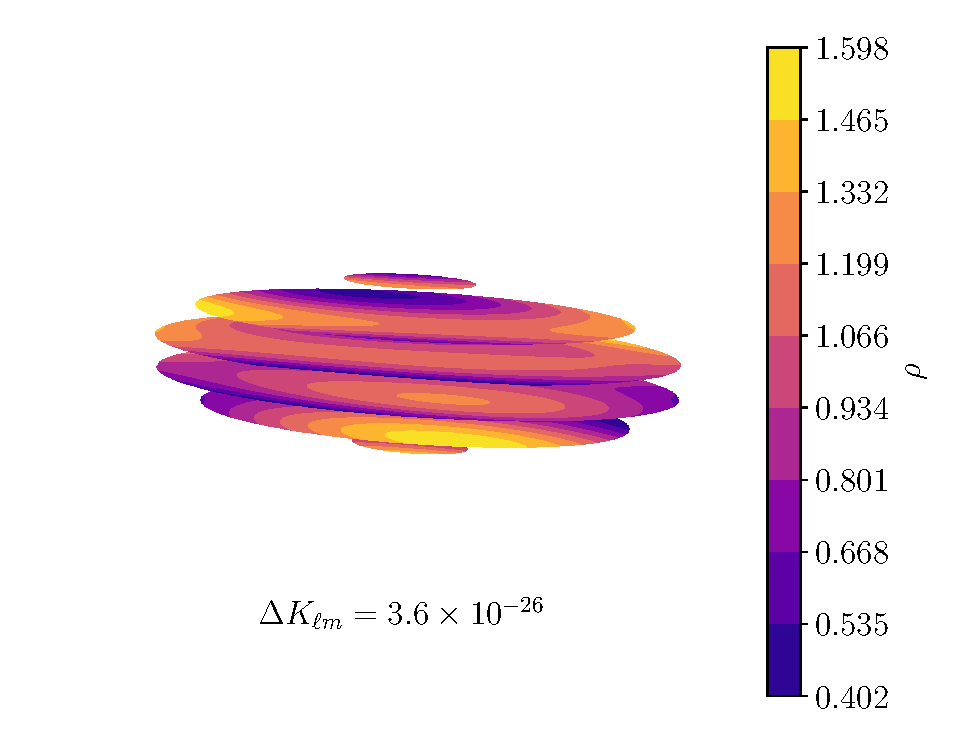
\includegraphics[width=0.33\textwidth]{figs/asym-ell-likelihood.pdf}\hfill
  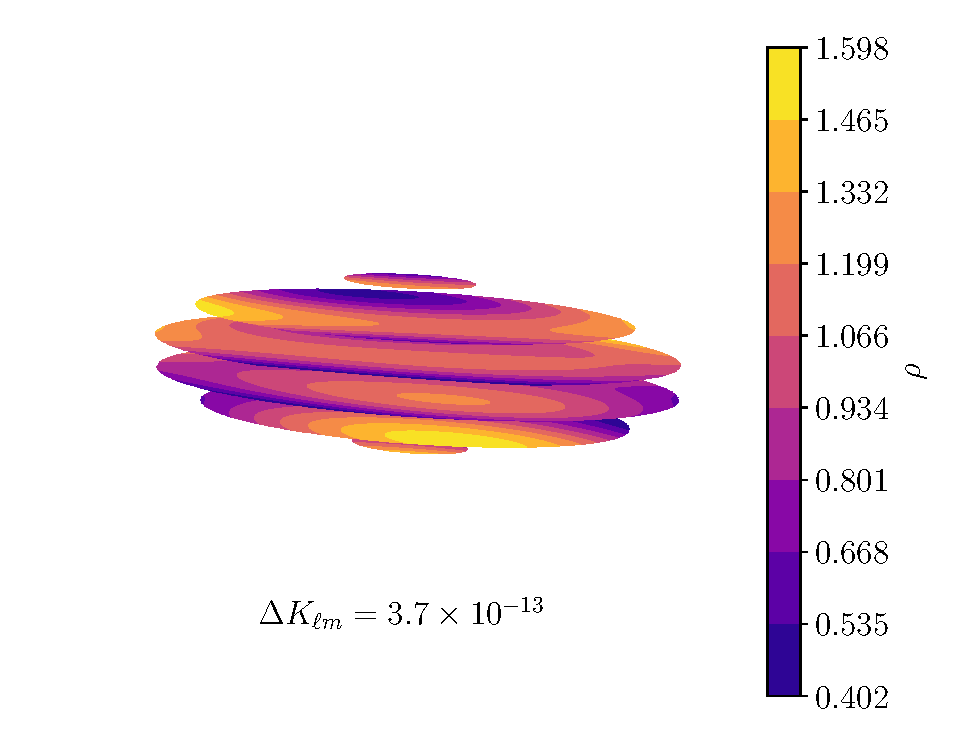
\includegraphics[width=0.33\textwidth]{figs/asym-ell-harmonic.pdf}\hfill
  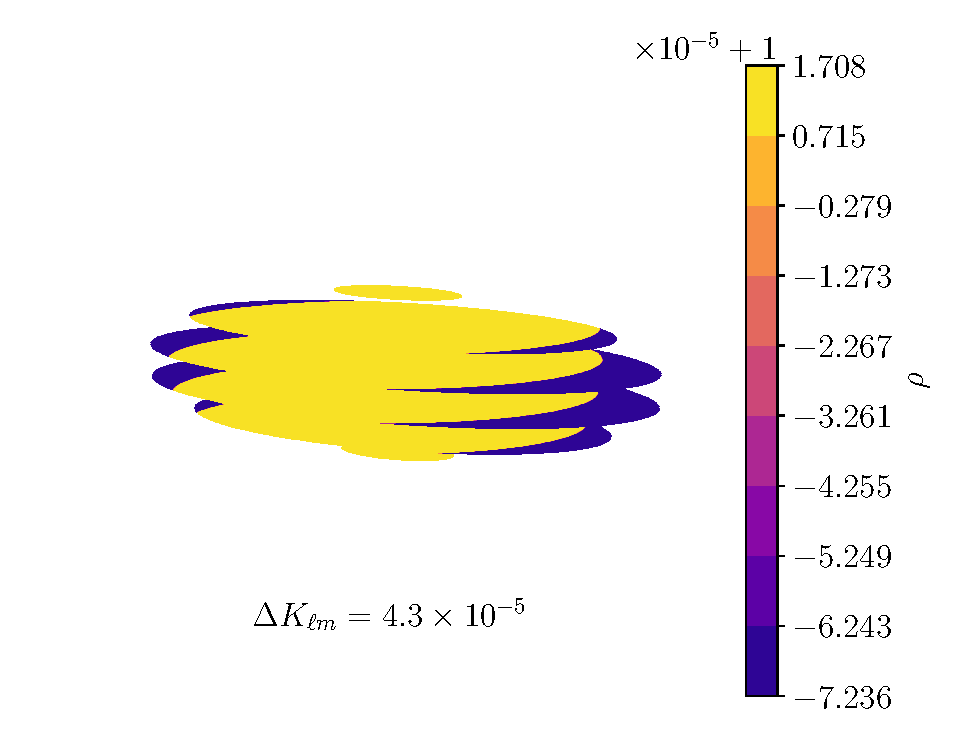
\includegraphics[width=0.33\textwidth]{figs/asym-ell-lumpy.pdf}

  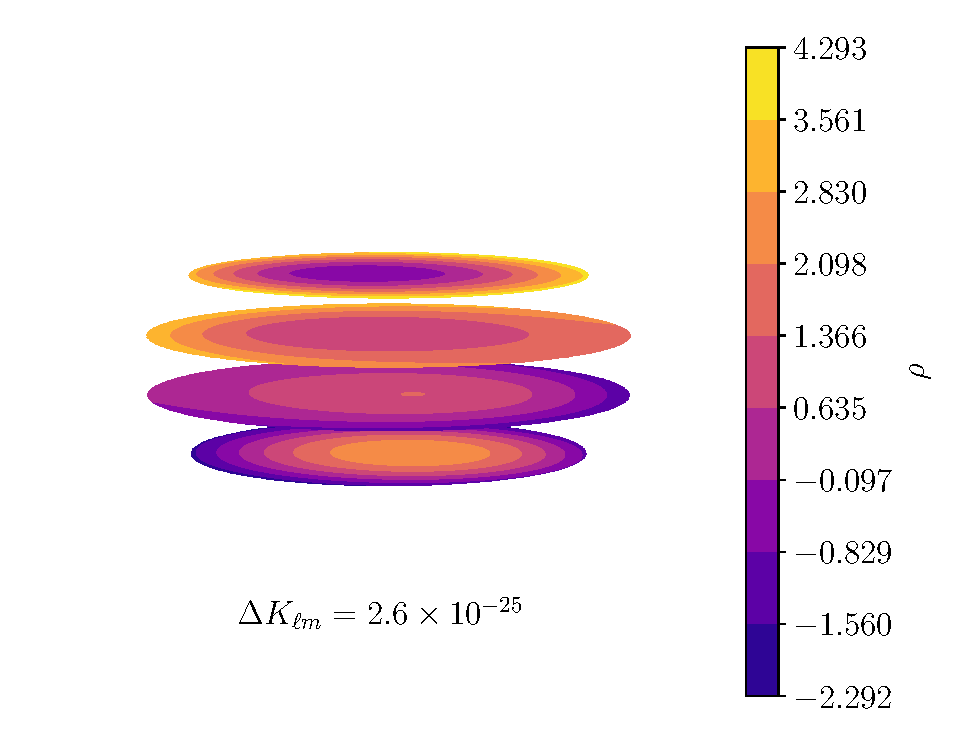
\includegraphics[width=0.33\textwidth]{figs/sym-ell-likelihood.pdf}\hfill
  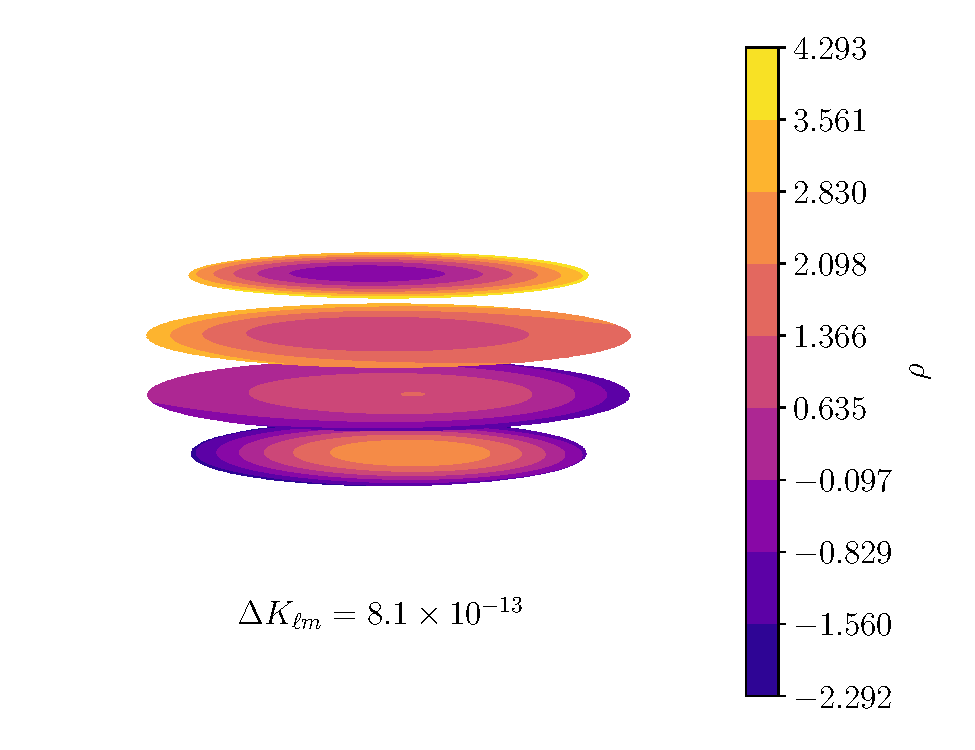
\includegraphics[width=0.33\textwidth]{figs/sym-ell-harmonic.pdf}\hfill
  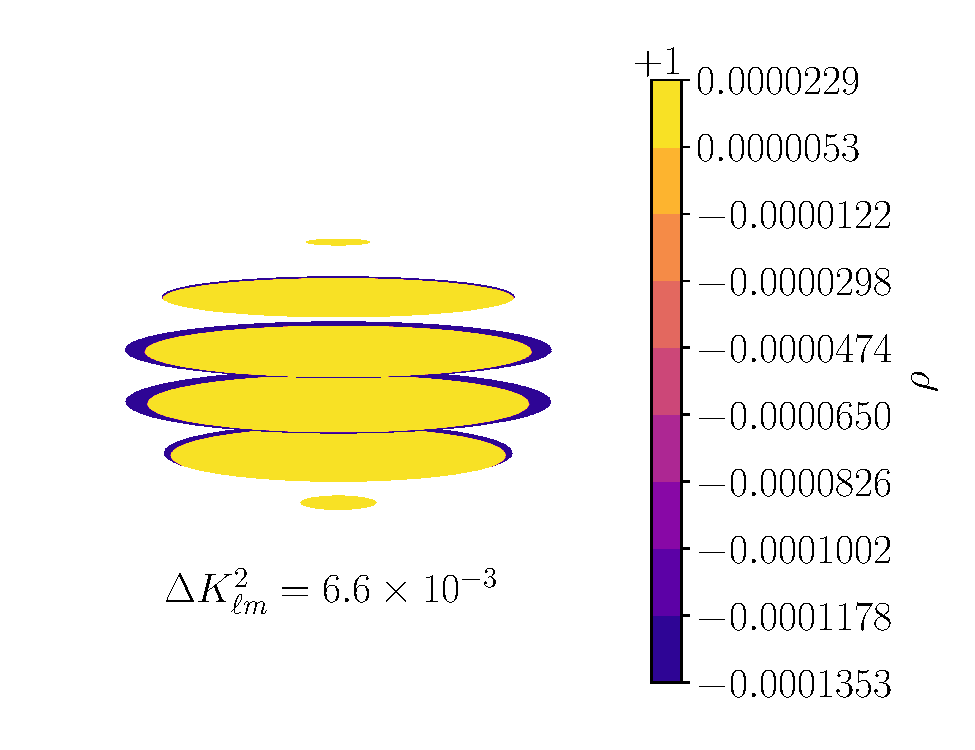
\includegraphics[width=0.33\textwidth]{figs/sym-ell-lumpy.pdf}

  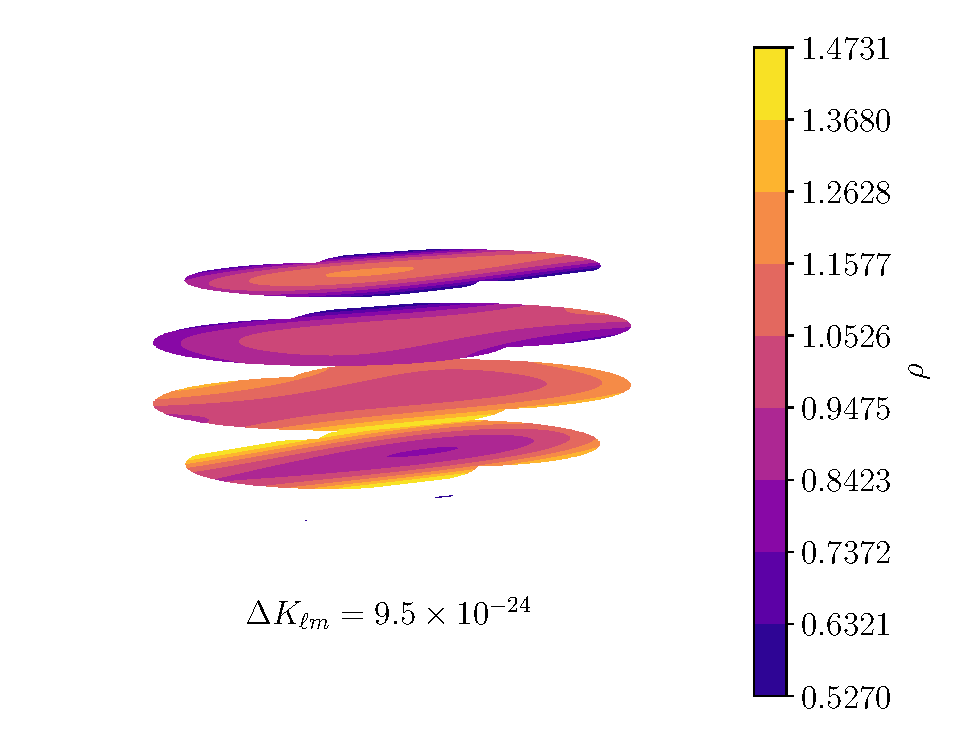
\includegraphics[width=0.33\textwidth]{figs/db-likelihood.pdf}\hfill
  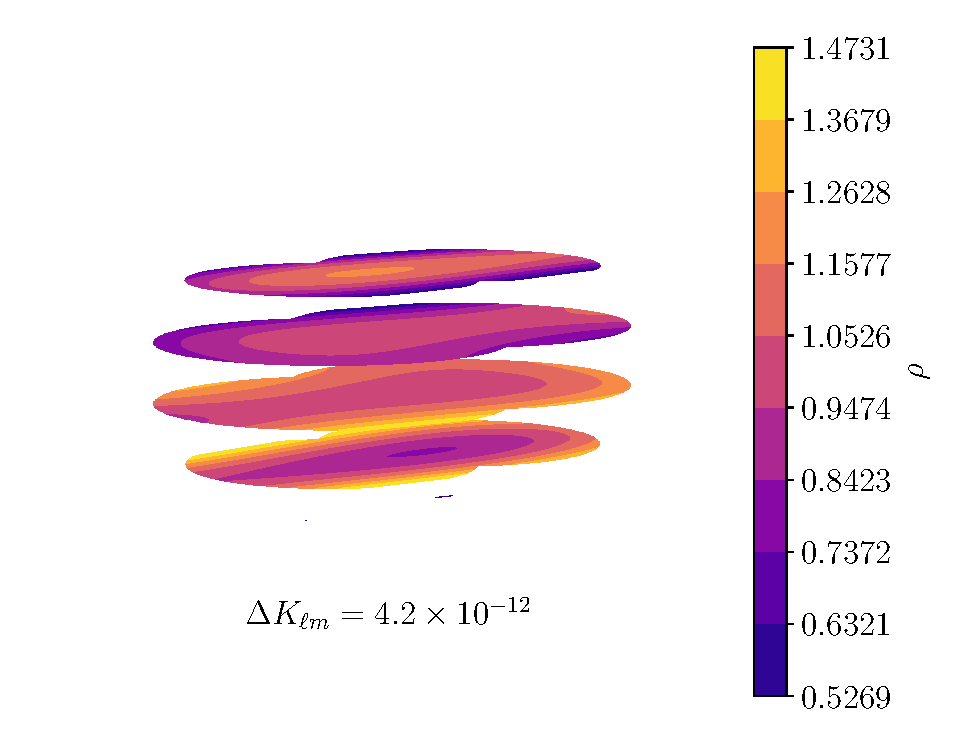
\includegraphics[width=0.33\textwidth]{figs/db-harmonic.pdf}\hfill
  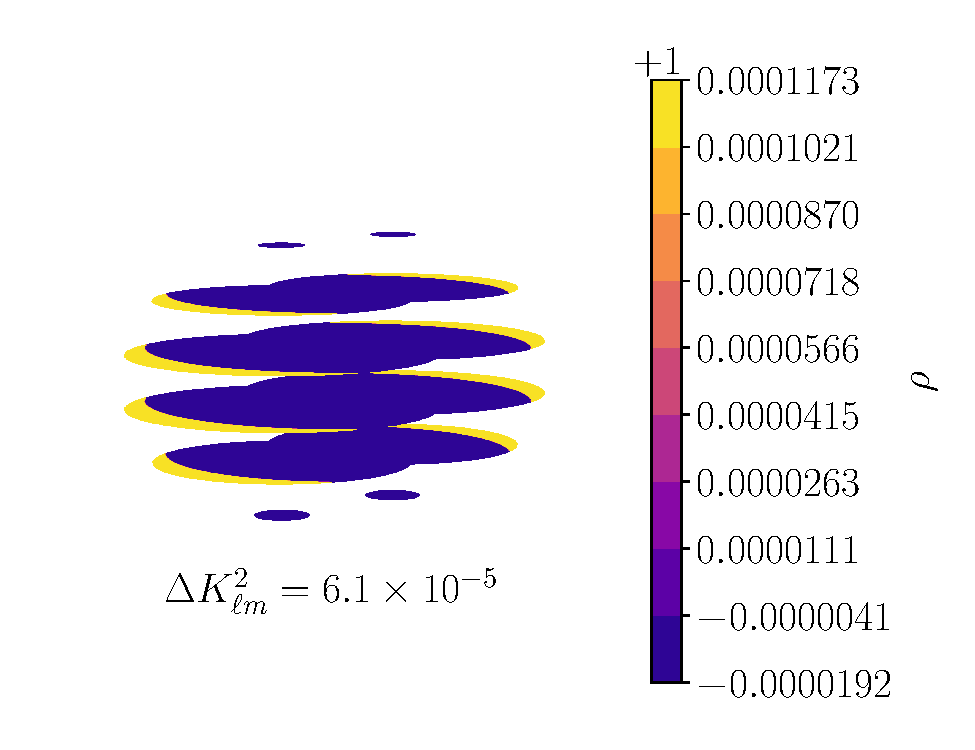
\includegraphics[width=0.33\textwidth]{figs/db-lumpy.pdf}

  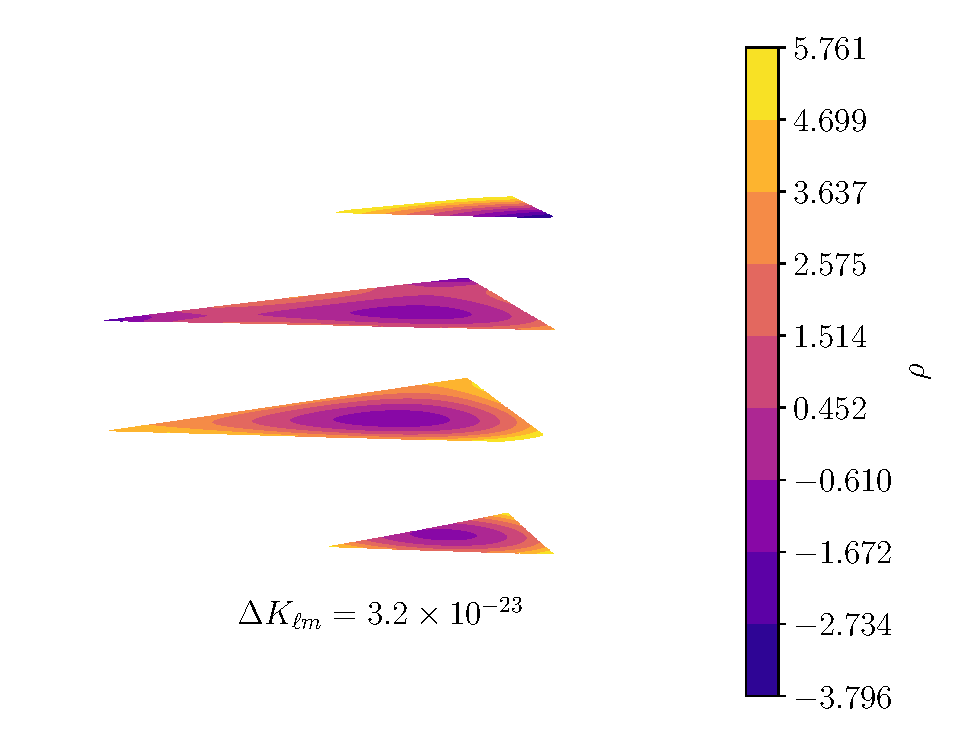
\includegraphics[width=0.33\textwidth]{figs/tet-likelihood.pdf}\hfill
  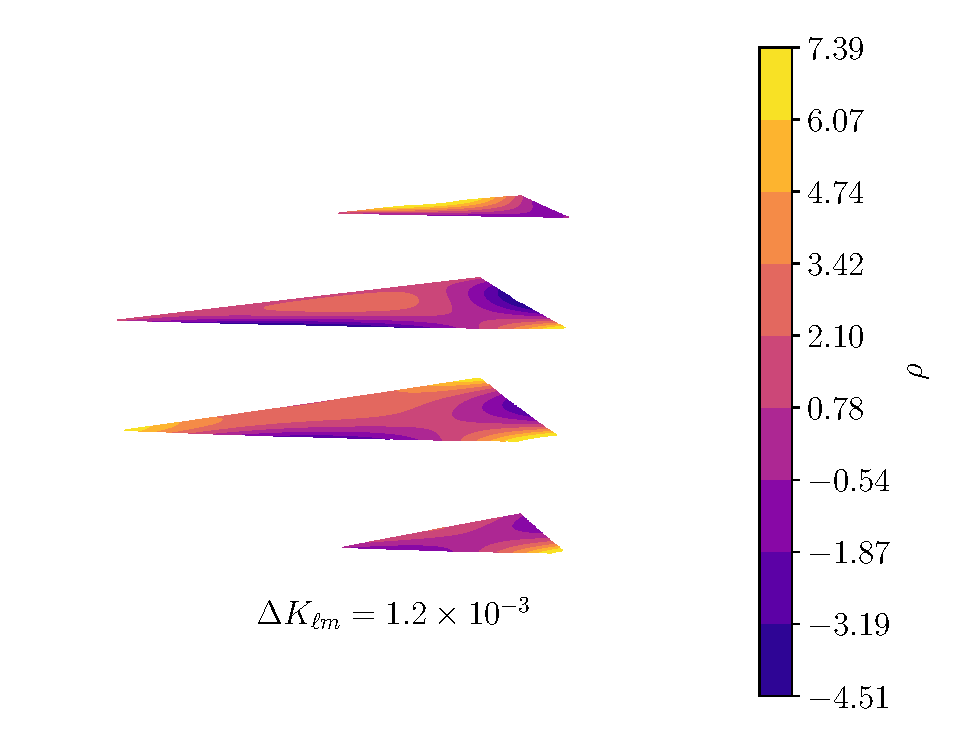
\includegraphics[width=0.33\textwidth]{figs/tet-harmonic.pdf}\hfill
  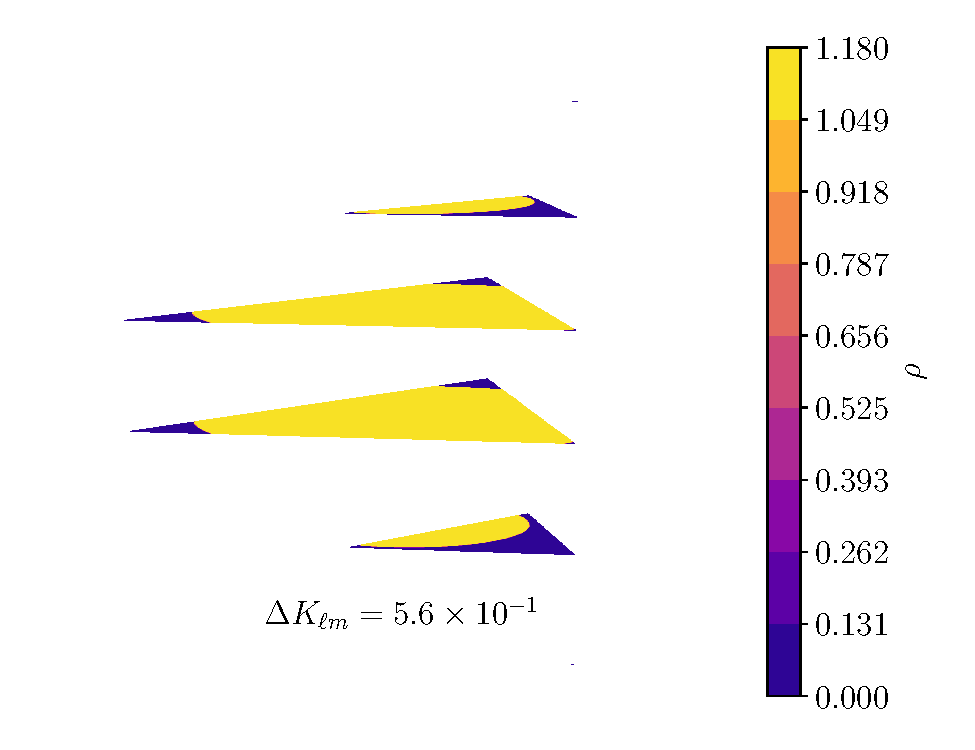
\includegraphics[width=0.33\textwidth]{figs/tet-lumpy.pdf}
  \caption{Density distributions extracted by the likelihood (\textit{left}), harmonic (\textit{middle}), and lumpy with $d=N=1$ (\textit{right}) models from data generated for a uniform-density asteroid. The asteroid shapes are, from top to bottom, the reference asymmetric ellipsoid, the reference symmetric asteroid, the dumbbell model, and a tetrahedron. Density is normalized so that mean density is one. The same distance scale is used in all figures.}
  \label{fig:uniform-density}
\end{figure*}

From figure \ref{fig:uniform-density}, it can be seen that the likelihood and harmonic models produce mostly the same density distributions. This is generally true for uniform density asteroids, which have harmonic density distributions. Consequentially, $\Delta K_{\ell m}$ is low for the harmonic model. This similarity lends confidence that the models produced are truly representative of the asteroid since they are produced via two independent methods.

The asymmetric and dumbbell asteroids produce distributions whose non-uniformity is limited to a factor of 2 or less for the harmonic and likelihood models. This non-uniformity is driven by error in the estimates of the density moments. Note that most of the asteroid has density close to one in both cases, with the factor of two reached only by small regions. The lumpy model yields a much more uniform distribution, because it is designed to produce uniform lumps. Note that its uncertainty $\Delta K_{\ell m}$ is usually large, both because the model is severely overdetermined (it has 2 degrees of freedom) and because the lump found extends outside the asteroid, violating the assumptions of the model. This is a sign that the lump found does not really exist inside the asteroid.

The symmetric and tetrahedral asteroids are less-well represented by the density distribution model results. In both cases, the likelihood and harmonic models produce sometimes-negative distributions, and non-uniformity is especially large in the tetrahedral case. This is not the fault of the density models, but rather because both of these asteroids have $K_{22} = 0$ and (as discussed in section \ref{sec:scan-shape}), this leads to degeneracy in $\gamma_0$ and inflated uncertainty in the density moments. In the tetrahedral case, the problem is worsened because $K_{20}=0$ as well, so that torque is dominated by the small and ill-constrained $K_{3m}$ components.

Uncertainty in each distribution was calculated but not shown. The size of uncertainty is such that the density distribution is consistent with uniform at most points for all models(within 1-2$\sigma$), with a small number of low-uncertainty regions that are less consistent with uniform. Uncertainty is generally larger towards the edges of the distribution, both for these shapes and for the shapes shown in the following sections.

From these examples, we may draw the conclusions that all three models produce density distributions generally consistent with uniform for uniform asteroids. The most likely distributions (i.e., the ones shown in the figures) are themselves mostly uniform, but can still produce non-uniformities as large as a factor of 2 in certain regions due to uncertainty in $K_{\ell m}$. Asymmetric asteroids such as the dumbbell and the asymmetric reference asteroids yield the best results because they have $K_{22} \neq 0$ and therefore do not suffer from degeneracy in initial orientation. Finally, the lumpy model can generally be ruled out in these cases because it produces unphysical results.

If desired, the parameters of the models can be reduced to only fit the $K_{2m}$ density moments; this will produce exactly uniform distributions, since it is equivalent to assuming $K_{3m}=0$. However, doing so ignores the observational insight we gain from our fits to $K_{3m}$, so it is only valid when $K_{3m}$ are too poorly constrained to be used. 

\subsubsection{Spherical shape test}
\label{sec:spherical-density}
We test the sensitivity of the density distributions to incorrect estimates for the shape of the asteroid by obtaining density moments from an ellipsoidal asteroid encounter and extracting density distributions assuming a spherical shape. We do this for the asymmetric and symmetric reference asteroids, with density distributions shown in figure \ref{fig:sphere-density}.

\begin{figure*}
  \centering
  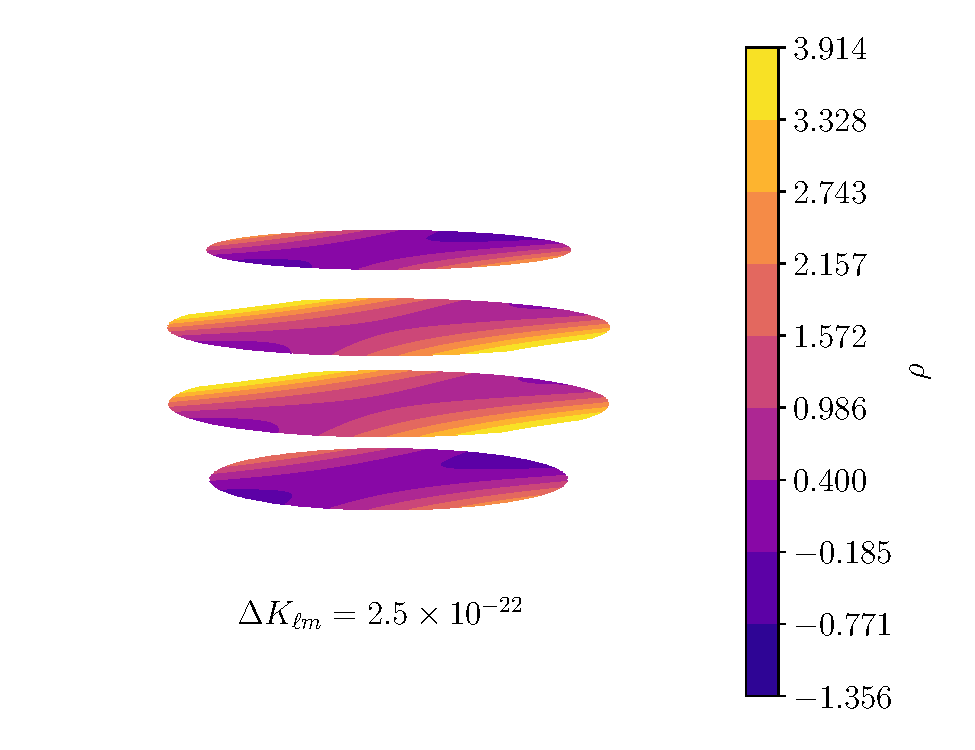
\includegraphics[width=0.33\textwidth]{figs/asym-sph-likelihood.pdf}\hfill
  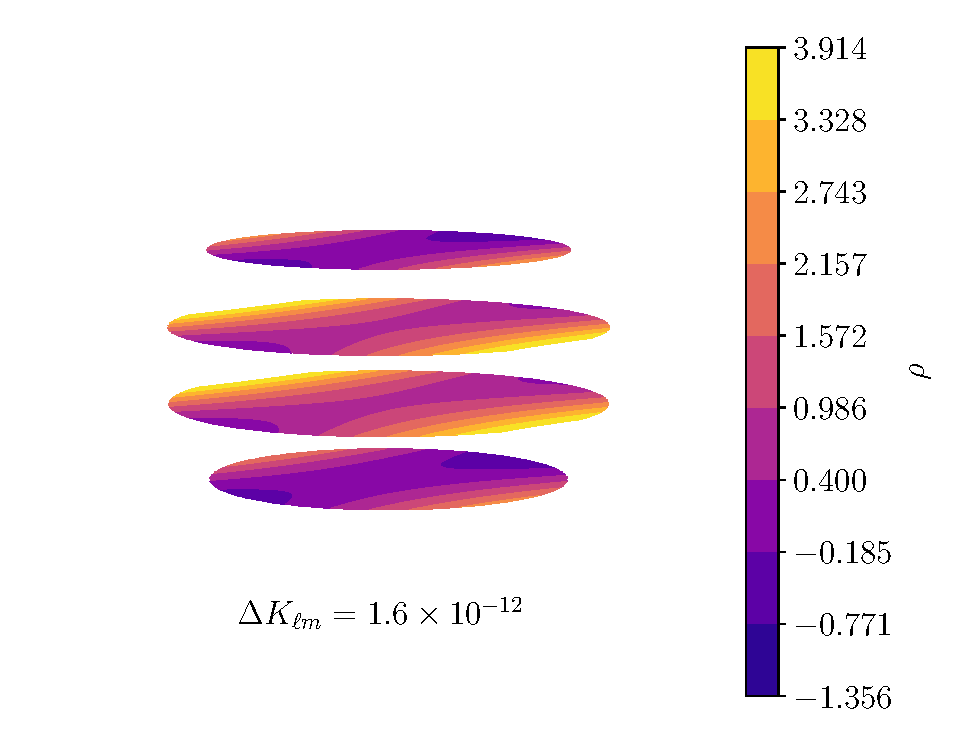
\includegraphics[width=0.33\textwidth]{figs/asym-sph-harmonic.pdf}\hfill
  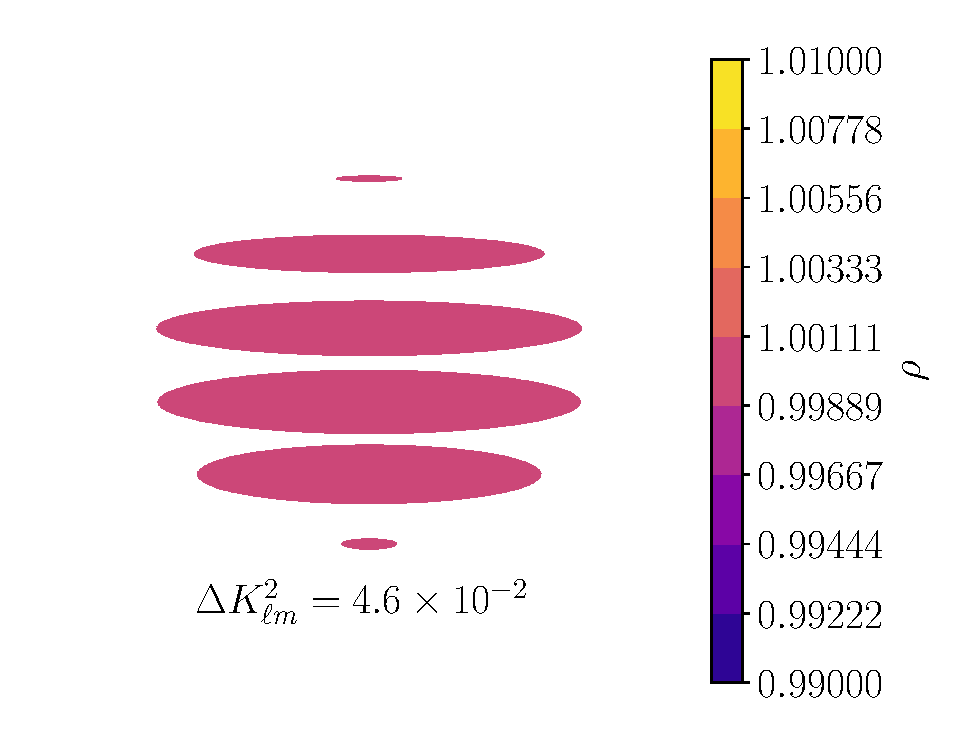
\includegraphics[width=0.33\textwidth]{figs/asym-sph-lumpy.pdf}

  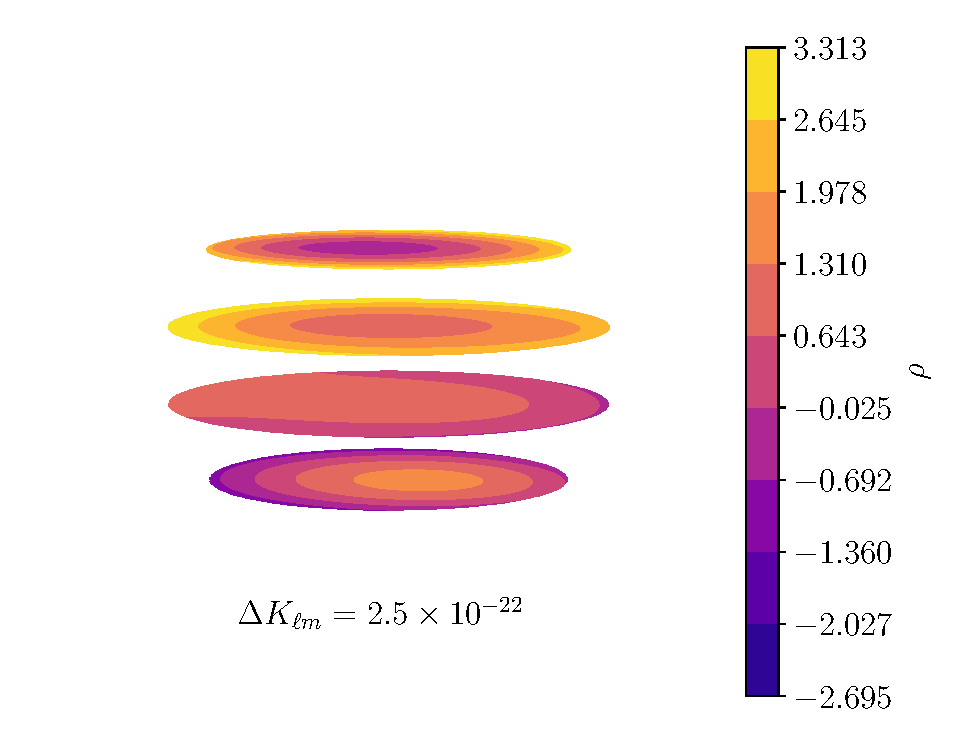
\includegraphics[width=0.33\textwidth]{figs/sym-sph-likelihood.pdf}\hfill
  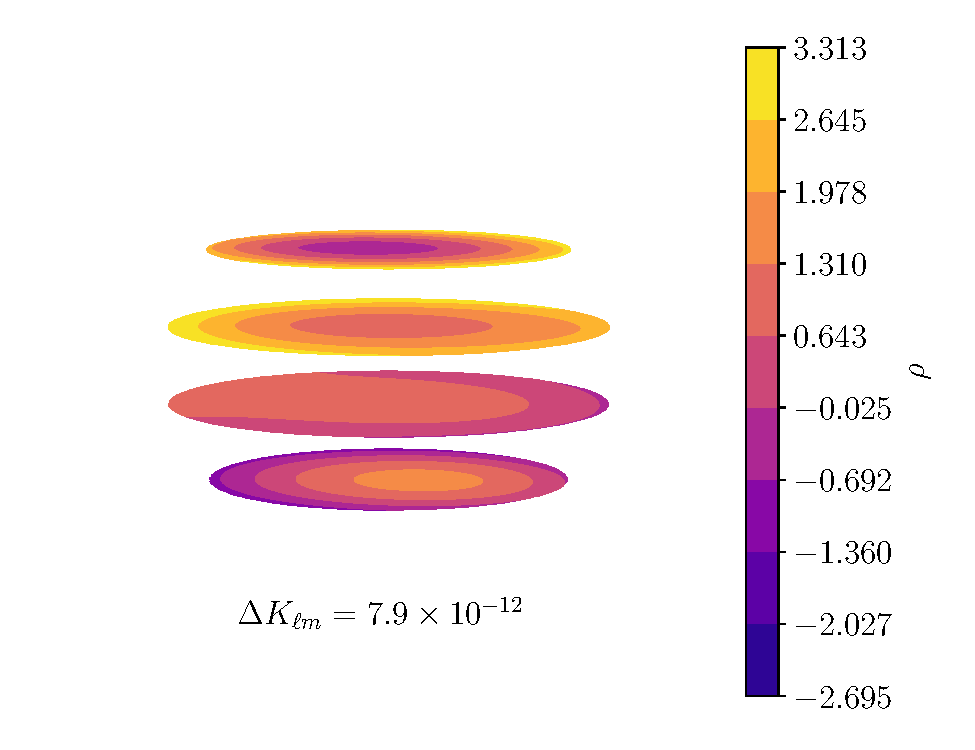
\includegraphics[width=0.33\textwidth]{figs/sym-sph-harmonic.pdf}\hfill
  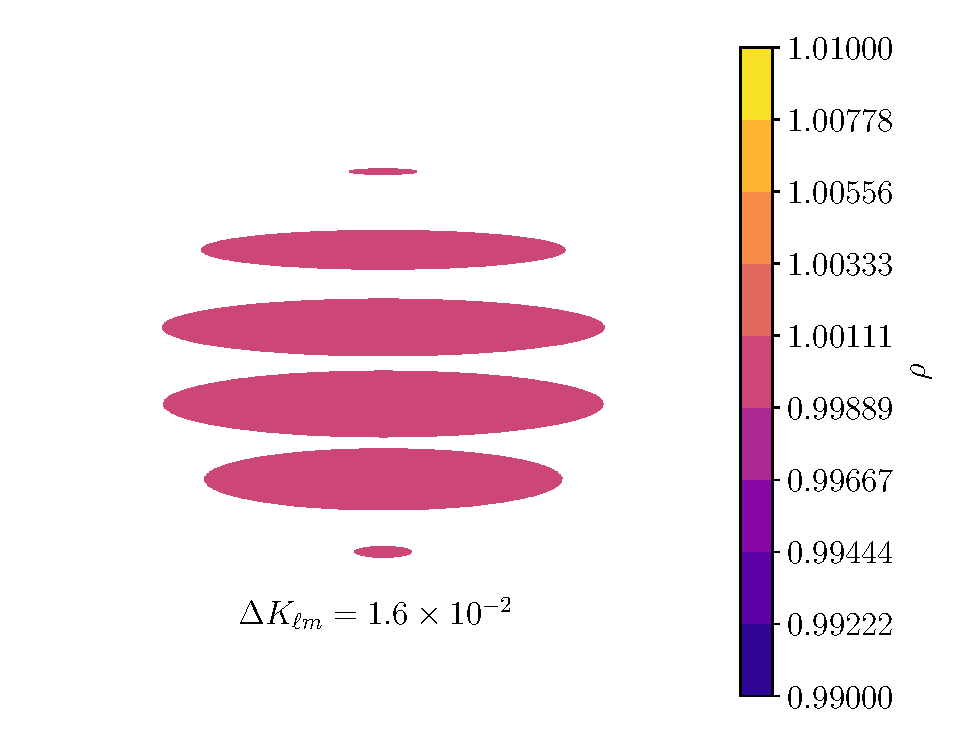
\includegraphics[width=0.33\textwidth]{figs/sym-sph-lumpy.pdf}\

  \caption{Density distributions extracted by the likelihood (\textit{left}), harmonic (\textit{middle}), and lumpy with $d=N=1$ (\textit{right}) models from data generated for a uniform-density asteroid. The original asteroid shapes were the reference asymmetric (\textit{top}) and symmetric (\textit{bottom}) ellipsoids. In both cases, the density distributions have been extracted assuming a spherical shape. Density is normalized so that mean density is one. The same distance scale is used in all figures.}
  \label{fig:sphere-density}
\end{figure*}

Both the likelihood and harmonic models are accurate in that $\Delta K_{\ell m}$ is low, and they produce similar distributions as in the previous section. However, now they both produce negative density distributions for both asteroid shapes. (In the previous section, only the symmetric model did.) This is a signal that the shape model is incorrect, and indeed the density distribution allows us to determine exactly how the shape model is wrong. In the asymmetric ellipsoid case, the density distribution is small (even negative) at large $|z|$ (top and bottom of the figure). The density is large at large $|y|$ (front right and back left in the figure). Comparison with the asymmetric reference asteroid depicted in figure \ref{fig:uniform-density} shows that the low-density region is outside the true asteroid shape, and the high-density region is inside. In other words, the shape can be corrected by extending it where density is large and retracting it where density is low.

A similar statement is true for the symmetric ellipsoid case in that density is low near the poles, but this time the regions with large density are evenly distributed around the equator, indicating the symmetry of the original asteroid.

The lumpy model produces lumps so large that they dominate the asteroid, predicting uniform distribution with $K_{\ell m} = 0$ for $\ell \geq 1$. The error in density moments $\Delta K_{\ell m}$ is therefore very large, equal to the sum of $|K_{\ell m}|$ for the original asteroids, making it clearly a poor model.

In short, severely incorrect shape estimates can be caught for all three models by negative predicted densities or by the failure of the density distribution model to match the extracted density moments. The shape can be corrected by extending it where the density distribution is high and retracting it where the density distribution is low.


\subsubsection{Nonuniformity test}
\label{sec:non-uniform-density}

We also test several non-uniform density asteroids and compare the generated density distributions for all three models to see if the non-uniformities are recovered. We consider two asteroids, one with mass concentrated in the middle, and one with mass concentrated around the edges. (Specifically, the mass distribution follows a spherically symmetric exponential $\rho(r) \propto e^{\pm r^2/a_\mathcal{A}^2}$). To prevent the problems seen in previous sections when a symmetric asteroid is simulated, we set the shape of the asteroids to the asymmetric reference asteroid. The extracted density distributions are shown in figure \ref{fig:non-uniform-density}

\begin{figure*}
  \centering
  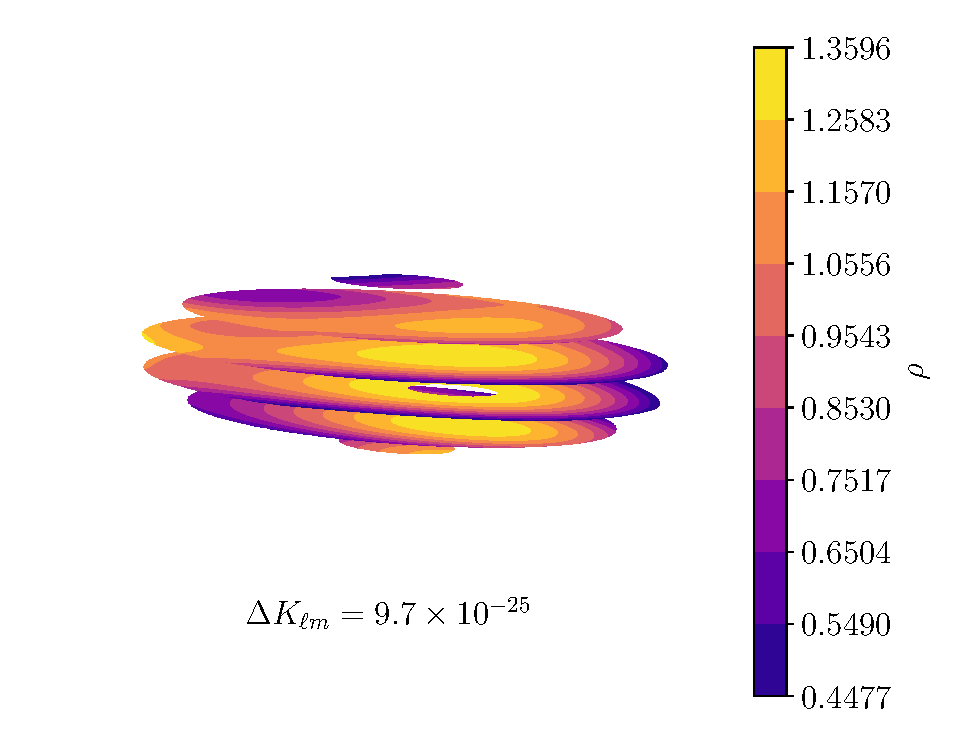
\includegraphics[width=0.33\textwidth]{figs/in-likelihood.pdf}\hfill
  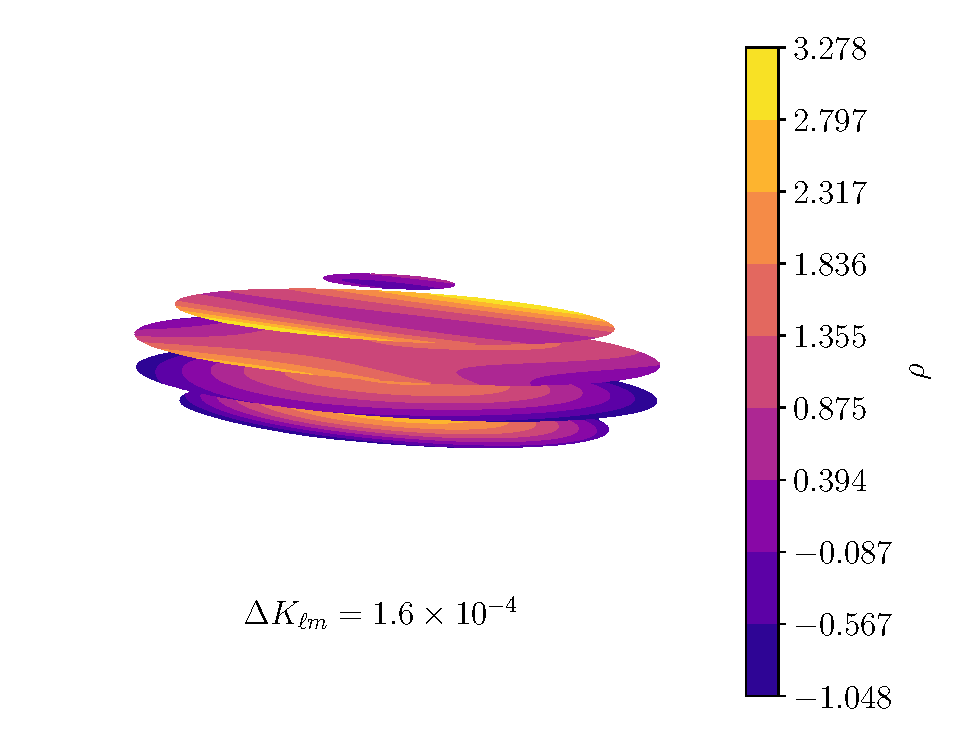
\includegraphics[width=0.33\textwidth]{figs/in-harmonic.pdf}\hfill
  \includegraphics[width=0.33\textwidth]{figs/in-lumpy.pdf}

  \includegraphics[width=0.33\textwidth]{figs/out-likelihood.pdf}\hfill
  \includegraphics[width=0.33\textwidth]{figs/out-harmonic.pdf}\hfill
  \includegraphics[width=0.33\textwidth]{figs/out-lumpy.pdf}\

  \caption{Density distributions extracted by the likelihood (\textit{left}), harmonic (\textit{middle}), and lumpy with $d=N=1$ (\textit{right}) models from data generated for non-uniform-density asteroids with mass concentrated in the middle (\textit{top}) and the edges (\textit{bottom}).Density is normalized so that mean density is one. The same distance scale is used in all figures.}
  \label{fig:non-uniform-density}
\end{figure*}

For these non-uniform asteroids, the likelihood and harmonic model do not coincide, as can be seen by comparing the density distributions and the fact that $\Delta K_{\ell m}$ is much larger for the harmonic distribution (indicating that the true density distribution is not harmonic). However, the two models do give similar results. Comparing the centre-weighted asteroid and the edge-weighted asteroid distributions, one can see that the centre-weighted case indeed places more mass in the centre of the asteroid shape for the harmonic and likelihood models, while the edge-weighted asteroid places mass at the edges.

Though these general trends in mass placement arrived at by both the likelihood and harmonic models are accurate, the precise density distributions are inaccurate because they predict negative densities. This might be addressed for the likelihood model by selecting a likelihood that strongly disfavours negative densities, such as a log-normal distribution. A log-normal likelihood however would no longer yield a linear model, so we do not use one here.

Figure \ref{fig:non-uniform-density} shows that the lumpy model places one large lump of greater density than the surrounding medium for the centre-weighted asteroid and less density for the edge-weighted asteroid, as expected. Greater error is incurred in $\Delta K_{\ell m}$ in this lumpy model than for the harmonic and likelihood models due to the lumpy model's crudeness, but the lump gives a good qualitative estimate of the density distribution of the asteroid which is useful for interpreting the other two models. This fact demonstrates that it can be illustrative to run the models with reduced degrees of freedom for the sake of simplicity, even if doing so yields less accurate distributions.


The lumpy model has one caveat that has not yet been mentioned, which applies for $N=d=1$ if (1) the centre of mass of the asteroid is the centroid of the asteroid shape and (2) the density moments of the asteroid shape are proportional to the fitted density moments. (1) guarantees that the lump will be placed at the origin and therefore will not contribute to $K_{\ell m}$ for $\ell \geq 1$, and (2) guarantees that the mass of the asteroid shape will be chosen such that the shape density moments exactly match the fitted density moments. The lump radius will then be set to zero because the fitted density moments are already matched. This zero-radius-lump result will occur even if the true density distribution has a large-radius lump at the origin. The lump model will therefore fail to recognize the lump in the true density distribution.

An example of this caveat applied is an elliptical lump inside an elliptical asteroid similar to the ones above. This is why, in the centre-weighted and edge-weighted density distributions, we specifically chose a spherically symmetric density distribution for our ellipsoidal asteroid shape, rather than an a distribution that conforms to the asteroid shape.



\subsubsection{Lump test}

Finally, we test an asteroid with a discrete change in density distribution (for example, a boulder), of the kind that the lumpy model is designed to detect. We place a spherical mass of density six times the density of the surrounding medium inside the asymmetric reference asteroid, slightly displaced along $\unit y$. The rest of the asteroid we set to uniform density. The density distributions found by the three model for this asteroid are shown in figure \ref{fig:blob-density}.

\begin{figure*}
  \centering
  \includegraphics[width=0.33\textwidth]{figs/blob-likelihood.pdf}\hfill
  \includegraphics[width=0.33\textwidth]{figs/blob-harmonic.pdf}\hfill
  \includegraphics[width=0.33\textwidth]{figs/blob-lumpy.pdf}

  \caption{Density distributions extracted by the likelihood (\textit{left}), harmonic (\textit{middle}), and lumpy with $d=N=1$ (\textit{right}) models from data generated for an asteroid with an off-centre lump. Density is normalized so that mean density is one. The same distance scale is used in all figures.}
  \label{fig:blob-density}
\end{figure*}

We see from figure \ref{fig:blob-density} that the harmonic and likelihood model fail completely to recover the presence or location of the lump. There appears to be a slight increase in density at roughly the correct location for both models, but this is a small effect Like figure \ref{fig:non-uniform-density}, we see that the harmonic and likelihood models do not agree exactly, and the failure of the harmonic model to exactly reproduce $K_{\ell m}$ suggests that the true distribution is not harmonic.

The failure of these models to find lumps is expected, since $K_{\ell m}$ is most sensitive to non-uniformities of characteristic size $\pi/(\ell + 1)$ radians in the polar direction, and $2\pi / (|m|+1)$ in the azimuthal direction by the definition of $Y_{\ell m}$. This lump is too small to be resolvable by $K_{3m}$, so we do not expect most models to find it.

However, the lumpy model computes the location and density of the mass very well. Some inaccuracies are induced by the uncertainty in $K_{3m}$, which changes the minimum of equation \ref{eqn:lump-minimize} such that the lump is displaced by 9 m along $\unit y$ from where it should be. This in turn causes a 70 m inaccuracy in the lump's radius. Nevertheless, the accuracy is still good compared to other models, and we conclude that the lumpy model is capable of recreating the location of lumps (except for the caveat mentioned in the previous section for distributions with $K_{\ell m}$ proportional to the asteroid shape's moments). But the ability of the lumpy model to place a lump does not guarantee the lump to actually exist, as was seen in the other asteroid distributions analysed here.

\section{Conclusions}

We assess the feasibility of extracting density moments and density distributions for a general asteroid encounters, and ask what encounter properties are necessary to obtain the most information about asteroid density.

We derived a novel, arbitrary-order equation for the tidal torque experienced by an asteroid during an encounter with a planet of arbitrary shape and mass distribution. The tidal torque equation (equation \ref{eqn:tidal-torque}) revealed that the rotational velocity of the asteroid over time depends strongly on $K_{\ell m}$ and the initial orientation.

We built a fast simulation for an asteroid encounter, truncating the equation at second-order, and used the simulation to extract first- and second-order density moments from synthetic spin pole data via a Markov Chain Monte Carlo fit. We observe the following general properties of the moments:
\begin{enumerate}
  \item The second-order moments $K_{3m}$ are generally a factor of $~\frac{a_\mathcal{A}}{r_p}$ more uncertain than the first-order moments, where $a_\mathcal{A}$ is the asteroid radius and $r_p$ is the perigee distance. For our reference asteroid, this fraction was about $10^{-5}$.
  \item Of the seven second-order moments, those that measure small-scale variations in density (i.e., $|m|$ is large) are generally less uncertain. It is often possible to measure $K_{3|m|}$ for large $m$ even when $K_{30}$ is not resolved.
  \item The oblateness of the central body cannot be ignored without generating incorrect density moment estimates, but a non-zero oblateness does not greatly increase the precision of the extracted moments except perhaps when a moon is present.
\end{enumerate}

We assessed the posterior uncertainty generated by the fit process by adjusting eleven parameters of an asteroid on an Earth encounter. The main conclusions are listed below.

\begin{enumerate}
  \item Highly precise rotational velocity data is required to produce precise second-order moments. Especially the uncertainty on the asteroid rotational period must be small compared to the uncertainty on asteroid spin pole.
  \item Large $a_\mathcal{A}$ is required for $K_{3m}$ resolution, though the size of $a_\mathcal{A}$ has no effect on $K_{2m}$. The threshold on $a_\mathcal{A}$ for the reference asteroid was $\sim$700 m for $K_{30}$ and $\sim$50 m for $K_{33}$.
  \item A close encounter is vital for accurate second-order moment extraction, though some of the second-order moments can still be required for more distant encounters, extending to about a third of a Lunar distance for the reference asteroid.
  \item This model will yield inflated uncertainties if the asteroid is rotationally symmetric around its rotating spin axis. In this case, a different parametrization should be used. 
  \item If the asteroid rotational period is too small, the asteroid will not tumble after perigee. This inhibits the precise determination of $K_{2m}$, though $K_{3m}$ are largely unaffected. For the reference asteroid, the threshold was about 4 hours (although $K_{30}$ will become unresolved at for periods smaller than 8 hours). For similar reasons, initial rotational velocities orthogonal to the orbital plane or in the plane and perpendicular to the perigee vector will yield poor-quality fits, though the spin pole effect is smaller than the effect of rotational period.
  \item The cadence of observation should be shorter than about 30 minutes (except $K_{30}$ will become unresolved for cadence longer than 10 minutes). Gaps of data can appear, specifically at perigee, but only for a little over an hour given 2 minute cadence before the posterior uncertainty greatly increases.
\end{enumerate}

If some of these conditions are not met, the first-order $K_{2m}$ moments may still be resolvable.

Finally, we present three fast, linear methods for extracting density distributions (together with uncertainties) from the density moments and the shape of the asteroid as obtained by light-curve analysis. The extracted density distributions largely are consistent with the true distributions in all cases we tested. Slight adjustments to $K_{3m}$ dramatically change the overall distribution, so that they are not very precise. Indeed, the models sometimes predict negative density (though more complicated models could be made not to). Errors in the shape estimate of the asteroid also distort the density distribution, but the resulting distributions provide hints as to exactly where the shape is incorrect. Large-scale properties of the asteroid's true distribution, such as whether the mass is located in the middle or on the edges, are often observable. Two of the models presented (the harmonic and lumpy models) are flexible in their number of parameters, so that if only these large-scale properties are necessary, a small set of parameters can be chosen to prevent over-fitting.

In the appendices, we answer more specific questions that might arise about the behaviour of the tidal torque system and the fit process.

\section*{Acknowledgements}

We warmly thank Emmanuel Jehin, Maxime Devogele, and Marin Ferrais for meeting with the authors to discuss this work, and pointing out possible future directions to take it. JTD would like to thank the Massachusetts Institute of Technology Undergraduate Research Opportunities Program (MIT UROP) office for funding his work for many semesters, and their flexibility in funding students from departments other than the source of funding. Much of the computation behind this paper was executed on MIT Supercloud's facilities.



%%%%%%%%%%%%%%%%%%%%%%%%%%%%%%%%%%%%%%%%%%%%%%%%%%
\section*{Data Availability}

The code used to generate data, fit density moments to it, and extract density distributions from the moments is available on \href{https://github.com/jack-dinsmore/asteroid-tidal-torque}{GitHub}, or by contacting JTD.



%%%%%%%%%%%%%%%%%%%% REFERENCES %%%%%%%%%%%%%%%%%%

\bibliographystyle{mnras}
\bibliography{asteroids.bib}



%%%%%%%%%%%%%%%%%%%%%%%%%%%%%%%%%%%%%%%%%%%%%%%%%%

%%%%%%%%%%%%%%%%% APPENDICES %%%%%%%%%%%%%%%%%%%%%

\appendix

\section{Tidal torque \& Equations of motion}
\label{app:eom}

In this appendix, we derive the equations of motion used to simulate the asteroid angular velocity during the encounter. In particular, we describe our coordinates (section \ref{sec:coordinates}) for an encountering asteroid's position and orientation, and we parametrize its density distribution via its density moments (section \ref{sec:moments}). Then we derive an arbitrary-order equation for tidal torque (section \ref{sec:tidal-torque}) and write the equations of motion for the system (section \ref{sec:eom}).

\subsection{Coordinates}
\label{sec:coordinates}

We make use of two frames of reference to model this system. One is the ``inertial frame,'' with axes denoted by $\unit{X}$, $\unit{Y}$, $\unit{Z}$ and origin placed at the central body's centre of mass. $\unit{X}$ points from the central body to the asteroid periapse, and $\unit{Z}$ points parallel to the orbit angular momentum. We assume that the mass distribution of the central body is known in this inertial frame.

Our second frame is the ``body-fixed'' frame, denoted by $\unit{x}, \unit{y}, \unit{z}$. Each axis in this frame is aligned with a principal axis and rotates with the asteroid, with its origin at the asteroid's centre of mass. For definiteness, we define $\unit{z}$ to be the principal axis with maximal MOI (this is the short axis mode, to use the vocabulary of Ref.~\cite{kaasalainen2001interpretation}). In general, we use capital letters to denote vectors in the inertial frame and lowercase vectors to denote vectors in the body-fixed frame.

The difference between the origins of the body-fixed and inertial frames is the position of the asteroid. We represent the relative orientations by $z-y-z$ Euler angles $\alpha$, $\beta$, and $\gamma$, such that a matrix $M$ rotating from the body-fixed to the inertial frame ($M\bm{r} = \bm{R}$) is given by
\begin{equation}
M = R_z(\alpha) R_y(\beta) R_z(\gamma).
\label{eqn:euler-angles}
\end{equation}
Here, $R_i(\theta)$ is a rotation around the unit vector $i$ by $\theta$ (figure \ref{fig:euler-angles}).

\begin{figure}
    \centering
    \begin{tikzpicture}
    \draw[-{Latex[length=3mm]}] (0, 0) -- (-4, 0) node[anchor=east] {$\unit x$};
    \draw[-{Latex[length=3mm]}] (0, 0) -- (2, -3) node[anchor=west] {$\unit y$};
    \draw[-{Latex[length=3mm]}] (0, 0) -- (0, 4) node[anchor=south] {$\unit z$};
    \draw[dashed, -{Latex[length=3mm]}] (0, 0) -- (3.7, -2) node[anchor=north] {};
    \draw[line width=0.5mm,-{Latex[length=3mm]}] (0, 0) -- (-0.5, -3) node[anchor=north] {$\unit X$};
    \draw[line width=0.5mm,-{Latex[length=3mm]}] (0, 0) -- (4, 1) node[anchor=south] {$\unit Y$};
    \draw[line width=0.5mm,-{Latex[length=3mm]}] (0, 0) -- (-1.6, 2.7) node[anchor=south] {$\unit Z$};
    \draw[->] (0.5, -0.75) arc (290:302:2.5);
    \draw (0.9, -0.9) node[anchor=center] {$\alpha$};
    \draw[->] (0, 1.2) arc (130:161:1.3);
    \draw (-0.3, 1.3) node[anchor=center] {$\beta$};
    \draw[->] (0.97, -0.52) arc (330:368:1.3);
    \draw (1.4, -0.25) node[anchor=center] {$\gamma$};
    %\draw[-{Latex[length=3mm]}] (0, 0) -- (0, 4) node[anchor=south] {$\unit Z$};
    %\draw[-{Latex[length=3mm]}] (0, 0) -- (4, 0) node[anchor=west] {$\unit Y$};
    %\draw[-{Latex[length=3mm]}] (0, 0) -- (-2, -2) node[anchor=east] {$\unit X$};
    \end{tikzpicture}
    \caption{$z-y-z$ Euler angles used in this work to express the orientation of the asteroid. Orientation is expressed as a rotation from the body-fixed axes (lowercase) to the inertial axes (bold lines and uppercase). The origins are co-located for demonstration purposes.}
    \label{fig:euler-angles}
\end{figure}


\subsection{Density moments}
\label{sec:moments}

The un-normalized spherical harmonics are defined as $Y_{\ell m}(\theta, \phi) = P_{\ell m}(\cos \theta)e^{im\phi}$, where $P_{\ell m}$ are the associated Legendre Polynomials without the Condon-Shortley phase. The regular and irregular spherical harmonics are further defined as
\begin{equation}
  \begin{split}
    S_{\ell m}(\bm r) &= (-1)^m (\ell - m)! \frac{Y_{\ell m}(\unit r)}{r^{\ell+1}} \\
    R_{\ell m} (\bm r) &= (-1)^m \frac{r^\ell}{(\ell + m)!} Y_{\ell m}(\unit r).
  \end{split}
\end{equation}
These spherical harmonics obey many useful identities summarized in Ref.~\cite{Gelderen1998TheSO}, which are also useful for quantum mechanics. They were used to define the density moments in equation \ref{eqn:klm}, which can be extended to the central body:
\begin{equation}
  \begin{split}
    &J_{\ell m} = \frac{a_\mathcal{B}^{2-\ell}}{I_\mathcal{B}} \int_\mathcal{B} d^3 r \rho_\mathcal{B}(\bm r) R_{\ell m}(\bm r)\\
  \end{split}
  \label{eqn:jlm}
\end{equation}
By contrast, $J_{\ell m}$ should be computed in the inertial frame. The length scale $a_\mathcal{B}$ and MOI scale $I_\mathcal{B}$ can be defined similarly to $a_\mathcal{A}$ and $a_\mathcal{B}$ in equations \ref{eqn:aa} and \ref{eqn:ia}, but they could also be set to any other scales of the same units, e.g. $a_\mathcal{B}$ equal to the central body radius and $I_\mathcal{B} = \mu_\mathcal{B}a_\mathcal{B}^2$, where $\mu_\mathcal{B}$ is the central body mass.

Note that both $J_{\ell m}$ and $K_{\ell m}$ are unitless. We call them ``moments'' because the $R_{\ell m}(\bm r)$ contains an $r^\ell$ dependence so that $K_{\ell m}$ is the $\ell$th density moment of the asteroid.

These moments share several key properties which we discuss before continuing. Firstly, for real mass density, properties of the spherical harmonics imply that $K_{\ell m} = (-1)^m K_{\ell, -m}^*$. Therefore, the set of $K_{\ell m}$ for $\ell < \ell_\text{max}$ contains $\ell_\text{max}^2$ degrees of freedom. However, some of these degrees of freedom are redundant with the choice of coordinates: $K_{1m} = 0$ since the body-fixed frame is centred on the asteroid centre of mass. Further calculation reveals that the alignment of the body-fixed frame with the asteroid principal axes also forces $K_{21}= 0$ and $\Im K_{22}=0$. The only physical density moments for $\ell \leq 2$ are therefore $K_{22}$, $K_{20}$, and $K_{00}$. The first two are related to the MOI around each principal axis by equation \ref{eqn:moi}, while $K_{00} = \mu_\mathcal{A} a_\mathcal{A}^2 / I_\mathcal{A}$ will not be relevant to this study as it does not appear in equation \ref{eqn:tidal-torque}. 

The physical meaning of $K_{22}$ and $K_{20}$ can also be interpreted via a special case: if the asteroid is a uniform-density triaxial ellipsoid, the moments of inertia are simple to compute in terms of the semi-axis lengths and can be compared to those found in equation \ref{eqn:moi}. This yields semi-axis lengths of 
\begin{equation}
  \begin{split}
  a &= \sqrt{\frac{5}{3}}a_\mathcal{A}\sqrt{1-2K_{20}+12K_{22}}\\
  b &= \sqrt{\frac{5}{3}}a_\mathcal{A}\sqrt{1-2K_{20}-12K_{22}}\\
  c &= \sqrt{\frac{5}{3}}a_\mathcal{A}\sqrt{1+4K_{20}}.
  \label{eqn:ellipsoid-axes}
  \end{split}
\end{equation}
The higher-order moments $K_{3m}$ can be thought of loosely as measuring the large-scale asymmetries of the asteroid. An asteroid that is mirror-symmetric along the $\unit{x}$ axis (meaning $\rho_\mathcal{A}(x,y,z)=\rho_\mathcal{A}(-x,y,z)$) necessarily sets certain density moments to zero. Which density moments are zeroed by which mirror symmetries is outlined in table \ref{tab:klm-symmetries}. All $K_{3m}$ are zeroed by at least one mirror symmetry. 

\begin{table}
  \centering
  \begin{tabular}{c|ccccccc}
    \hline
    $\ell$ & $\Re K_{\ell 3}$ & $\Im K_{\ell 3}$ & $\Re K_{\ell 2}$ & $\Im K_{\ell 2}$ & $\Re K_{\ell 1}$ & $\Im K_{\ell 1}$ & $K_{\ell 0}$ \\ \hline
    0 &  &  &  &  &  &  & -\\ 
    1 &  &  &  &  & x & y & z\\ 
    2 &  &  & - & x,y & y,z & x,z & -\\ 
    3 & x,z & y,z & z & x,y,z & x & y & z\\ \hline
  \end{tabular}
  \caption{Axes of mirror symmetry that imply zeroed density moments. For example, for mirror symmetries along $\unit y$ or $\unit z$, $\Im K_{32}=0$. Mirror symmetry along $\unit x$ means $\rho_\mathcal{A}(x, y, z) = \rho_\mathcal{A}(-x, y, z)$. Dashes indicate that none of the mirror symmetries zero the moment in question. Since $r^2>0$ for $r\neq 0$, no symmetries set $a_\mathcal{A}=0$ either.}
  \label{tab:klm-symmetries}
\end{table} 

Finally, the requirement that $\rho_\mathcal{A}(\bm r) \geq 0$ everywhere restricts $K_{\ell m}$. In the case of $K_{2m}$, this fact and the constraint that $I_z$ is larger than $I_x$ or $I_y$ requires $K_{20}$ and $K_{22}$ to fall in the triangle
\begin{equation}
  -\frac{1}{4} \leq K_{20} \leq 0, \qquad |K_{22}| \leq -\frac{K_{20}}{2}.
  \label{eqn:parameter-bounds}
\end{equation}
An analytical constraint on $K_{3m}$ based on this property is more difficult to derive, but in practice, we also observe that $|K_{3m}| < 0.01$.




\subsection{Tidal torque}
\label{sec:tidal-torque}

Derivations for the tidal torque experienced by a rigid body in the gravitational field of a larger mass have been computed by several previous studies \cite{paul88,HouMar2017,BOUE2009750, ashenberg07}, often in terms of the MOI of the rigid body (or higher order moments of inertia), and to varying degrees of precision. A simple, first-order derivation is also easily computable in terms of the asteroid MOI in the inertial frame.

Here, we present a new derivation of the tidal torque to arbitrary orders in terms of the density moments of an asteroid defined in section \ref{sec:moments}. These density moments can be pre-computed and do not have to be re-evaluated every time-step.

The gravitational potential energy of the central body is, in its most general form,
\begin{equation}
V(\bm R') = -G\int_\mathcal{B} d^3 R \rho_\mathcal{B}(\bm R) \frac{1}{|\bm{R}-\bm{R'}|}.
\label{eqn:first-pe}
\end{equation}
where $\rho_\mathcal{B}$ is the density distribution of the central body and $\mathcal{B}$ indicates the central body's volume. All vectors here are written in the inertial frame. Given $|\bm{R}| < |\bm{R'}|$, Ref.~\cite{Gelderen1998TheSO} gives the identity
\begin{equation}
  \frac{1}{|\bm R - \bm R'|} = \sum_{\ell, m} R_{\ell m}(\bm R) S_{\ell m}^*(\bm R'),
  \label{eqn:ylm-expansion}
\end{equation}
where the sum is shorthand for $\sum_{\ell, m} = \sum_{\ell = 0}^\infty \sum_{m=-\ell}^\ell$.

Incidentally, it is the $|\bm R| < |\bm R'|$ assumption that inspires the assumption that there are ``no \textit{distant} perturbing objects'' (section \ref{sec:methods}). If a perturbing object such as a moon is not distant (i.e., it is closer to the system center of mass than the asteroid perigee so that $|\bm R| < |\bm R'|$ always), then it can be absorbed into $J_{\ell m}$ by equation \ref{eqn:jlm} and the assumptions of this derivation are not violated.

We are interested in translating the potential energy of equation \ref{eqn:first-pe} to the body-fixed frame. To do this, we let $\bm{R'} = \bm D + \bm U$, where $\bm D$ is the location of the asteroid in the inertial frame. We further define $\bm U = M\bm u$, where $\bm u$ is in the body-fixed frame and $M$ is the rotation matrix given by the Euler angles $\alpha$, $\beta$, and $\gamma$ (see section \ref{sec:coordinates}). The translation from $\bm {R'}$ to $\bm U$ is then attained by the identity 
\begin{equation}
  S_{\ell m}(\bm R') = \sum_{\ell', m'} (-1)^{\ell'}R^*_{\ell' m'}(\bm U)S_{\ell+\ell', m + m'} (\bm D),
  \label{eqn:ylm-translation}
\end{equation}  
provided by Ref.~\cite{Gelderen1998TheSO}, and from $\bm U$ to $\bm u$ is given by
\begin{equation}
  \begin{split}
    Y_{\ell m}(M\bm u) = \sum_{m'=-\ell}^\ell & (-1)^{m+m'}\sqrt{\frac{(\ell-m')!(\ell+m)!}{(\ell+m')!(\ell-m)!}} \\
    & \times \mathcal{D}^\ell_{mm'}(M)^* Y_{\ell m'}(\bm u).\\
  \end{split}
  \label{eqn:ylm-rotation}
\end{equation}
Here, $\mathcal{D}^\ell_{mm'}(M)$ are the Wigner-$D$ matrices, which are determined by the Euler angles $\alpha$, $\beta$, and $\gamma$ of $M$.

Equations \ref{eqn:first-pe} to \ref{eqn:ylm-rotation} then provide formula for $V(\bm u)$ expressed as a sum of integrals over $\mathcal{B}$ of the central body density $\rho_\mathcal{B}(\bm R)$ times $R_{\ell m}(\bm R)$. These are expressed via equation \ref{eqn:jlm} as $J_{\ell m}$.

The tidal torque experienced by the asteroid (in the body-fixed frame) is given by
\begin{equation}
  \bm{\tau}(\bm u) = \int_\mathcal{A} d^3 u \rho_\mathcal{A}(\bm u) (\bm u \times (-\nabla_{\bm u} V(\bm u)))
\end{equation}
where $\rho_\mathcal{A}$ is the density distribution of the asteroid and $\mathcal{A}$ indicates the volume of the asteroid. Making use of one more identity concerning the derivatives of spherical harmonics:
\begin{equation}
  \begin{split}
  \bm u \times \nabla R_{\ell m}(\bm u)=&\frac{1}{2}\Big[(i\unit x - \unit y)(\ell-m+1)R_{\ell,m-1}(\bm u)\\
  &+(i\unit x+\unit y)(\ell+m+1)R_{\ell,m+1}(\bm u)\\
  & +2im\unit z R_{\ell m}(\bm u)\Big],
  \end{split}
\end{equation}
tidal torque can now be expressed as a function only of the constants $J_{\ell m}$, $K_{\ell m}$, $a_\mathcal{A/B}$, $I_\mathcal{A/B}$, and the asteroid orientation and position (equation \ref{eqn:tidal-torque}). Some $K_{\ell m}$ terms are written in this equation with $|m|>\ell$; these should all be taken to be zero.

\subsection{Equations of motion}
\label{sec:eom}


The equations of motion of the asteroid position $\bm D$ are given by Newton's law of gravitation
\begin{equation}
  \dot{\bm V} = -\frac{G \mu_\mathcal{B}}{D^3} \bm D \qquad \dot{\bm D} = \bm V
  \label{eqn:pos-eom}
\end{equation}
where $\bm V$ is the asteroid velocity in the inertial frame. Rather than derive equations of motion for the Euler angles (which suffer from gimbal lock), we instead represent the orientation of the asteroid with a quaternion $\quat q$ which can be converted into Euler angles to compute $\mathcal{D}(\alpha, \beta, \gamma)$. This quaternion evolves as 
\begin{equation}
  \dot{\quat q} = \frac{1}{2}\quat q\quat \omega.
  \label{eqn:quat-eom}
\end{equation}
for angular velocity $\bm \omega$ given in the body-fixed frame. The equations of motion of $\bm \omega$ in turn are given by
\begin{equation}
  \begin{split}
    I_x \dot \omega_x - \omega_y \omega_z (I_y - I_z) &= \tau_x\\
    I_y \dot \omega_y - \omega_z \omega_x (I_z - I_x) &= \tau_y\\
    I_z \dot \omega_z - \omega_x \omega_y (I_x - I_y) &= \tau_z.
  \end{split}
  \label{eqn:omega-eom}
\end{equation}
Equations \ref{eqn:tidal-torque}, \ref{eqn:moi}, and \ref{eqn:pos-eom} to \ref{eqn:omega-eom} form a set of non-linear, first-order coupled differential equations in which can be numerically integrated. They are expressed in terms of the physical parameters $I_\mathcal{A/B}$, $a_\mathcal{A/B}$, $J_{\ell m}$, and $K_{\ell m}$ which are constant if the asteroid is rigid and the central body does not rotate.






\section{Comparing orientation and angular velocity data}

To extract the density distribution of an asteroid, the main text assumes that the angular velocity data of the asteroid is observable. It is possible that the orientation of the asteroid may be better constrained by observations than angular velocity. In this appendix, we generate an orientation data set for the reference asteroid flyby, extract a density distribution from it, and compare the results to distributions extracted from angular velocity data.

\subsection{Uncertainty model}
The likelihood used by the MCMC (equation \ref{eqn:log-likelihood}) requires redefinition in order to extract density moments from orientation data. This requires a new model for the uncertainty of orientation observations.

For the sake of this appendix, we will assume that all observations of orientation $O$ differ from the true orientation $O^*$ by a rotation by some angle $\phi$ around an axis drawn from a uniform distribution on the unit sphere, where $\phi$ is drawn from a normal distribution with mean zero and standard deviation $\sigma_\phi$. Expressing orientation as a quaternion $\quat q = q_r + q_i \bm i + q_j \bm j + q_k \bm k$, $\phi$ can be extracted and the likelihood written as 
\begin{equation}
  \ln \mathcal{L} = -\frac{2}{\sigma_\phi^2}\sum_{i=0}\parens{\cos^{-1}\left|\brackets{\quat q_i (\quat q_i^*)^{-1}}_r\right|}^2
  \label{eqn:orientation-like}
\end{equation}
where $\quat q_i$ is the $i$th quaternion in the data set measured in the inertial frame, and $\quat q_i^*$ is the true quaternion. It is assumed that both quaternions have norm one.

\subsection{Moment uncertainty comparison}
With the likelihood defined, we generate both angular velocity and orientation data for the asymmetric reference asteroid configuration and extract $K_{\ell m}$ means and uncertainties for both data sets via the fit method defined in the main text. Due to the different uncertainty models used for the orientation and angular velocity data sets, this set-up does not allow direct comparison between the sizes of moment uncertainty for both data sets. If one data set yields more precise moments than the other, one could not determine whether the effect is due to increased observational precision in the data set or the use of a data type that better constrains density moments. However, the relative uncertainty of moments can be compared between the two data sets.

To make this comparison, we compute moment uncertainties $\sigma(K_{\ell m})$ for both data sets and also compute the mean value of $\sigma(K_{\ell m})$ over all fit parameters. We then scale the moment uncertainties attained from the angular velocity data set so that the mean uncertainty of its parameters is equal to that of the orientation data set. This is equivalent to simply choosing observational uncertainties for the angular velocity data set which yield density moments to the same precision as the observational data set, because figure \ref{fig:scan-observational} shows that density moment uncertainty $\sigma(K_{\ell m})$ is proportional to observational uncertainty. The resulting PPDs for the density moments of both data sets are displayed in figure \ref{fig:orientation-unc}, as well as their mean values relative to the true values.

\begin{figure}
  \centering
  \includegraphics[width=0.7\linewidth]{figs/orientation-unc}
  \caption{PPDs for each parameter as extracted from angular velocity (blue) and orientation (orange) data. First order parameters are shown in the top panel and second-order parameters in the bottom. Mean values are also shown as vertical lines. Both data produce similar constraints on parameters, except in the case of $\gamma_0$.}
  \label{fig:orientation-unc}
\end{figure}

The figure demonstrates that using orientation data rather than angular velocity data does not greatly affect the relative uncertainties of density moments, except in the case of $\gamma_0$. This is expected due to the following argument. If the initial orientation of the asteroid is known, then the orientation of the next data point can be determined by knowledge of the asteroid's angular velocity at that moment. Thus, an orientation data set can be produced from an angular velocity data set and vice versa given an initial asteroid orientation. This initial orientation is defined up to $\gamma_0$ by the assumption of no initial tumbling, so that the orientation data set will affect $\sigma(\gamma_0)$ most strongly.

A smaller effect observed in figure \ref{fig:orientation-unc} is that the orientation data set yields similar uncertainties for all density moments of fixed $\ell$, whereas the angular velocity data set tends to yield larger uncertainties for small $|m|$, which will alter the density uncertainty discussed in the next section. However, this has little effect on the density distributions extracted by the finite element model from the two PPDs shown in the figure. The average density uncertainty $\sigma_\rho / \rho$ are essentially equivalent between the two data sets, as is the distribution of density and density uncertainty extracted.




\section{Additional density distribution models}
\label{app:more-models}

Two models were discussed in section \ref{sec:density-distro} to translate density moment constraints into density distribution constraints. Here we outline two additional models, the nearly-uniform and the harmonic models, which are less conventional but still useable for extracting density distribution properties. Unlike the finite element and lumpy models discussed in the main text, these models will yield smooth distributions with no discrete transitions. They also rely on a known surface for the asteroid.

\subsection{Nearly-uniform model}
In this ``nearly-uniform'' model, we seek to pick one density distribution from the many distributions consistent with the data by maximizing a prior distribution $f[\rho(\bm r)]$, which can be chosen manually. Any prior distribution can be chosen, but the following prior is both interesting and numerically efficient.

As part of our prior, we require that the asteroid density distribution satisfy $I_\mathcal{A} = \mu_\mathcal{A} a_\mathcal{A}^2$. This constraint is desirable as it is obeyed for uniform density distributions. To define the prior, we divide the asteroid into $n \gg 1$ small regions of volume $V$, each with position $\bm r_i$ and density $\rho_i = \delta_i + 1$. Setting the mass of the asteroid equal to its volume, the average density is 1, so $\delta_i$ is the difference between the average and local density. We set $f[\rho(\bm r)]$ to be a multivariate-Gaussian distribution on $\delta_i$, centred on zero to minimize non-uniformity, i.e.
\begin{equation}
  f[\rho(\bm r)] \propto \prod_i \exp\parens{-\frac{\delta_i^2}{2\sigma^2}} \implies \ln f[\rho(\bm r)] \simeq -\sum_i \delta_i^2
  \label{eqn:nu-f}
\end{equation}
where $\sigma$ is an irrelevant constant. The density moments, MOI scale, and mass are 
\begin{equation}
  K_{\ell m} = \frac{V}{\mu_\mathcal{A}a_\mathcal{A}^{\ell}} \sum_i (\delta_i + 1) R_{\ell m}(\bm r_i)
  \label{eqn:nu-klm}
\end{equation}
\begin{equation}
  I_\mathcal{A} = \mu_\mathcal{A} a_\mathcal{A}^2 = V \sum_i (\delta_i + 1) r_i^2
  \label{eqn:nu-ia}
\end{equation}
\begin{equation}
  \mu_\mathcal{A} = V\sum_i (\delta_i + 1) \implies 0 = \sum_i \delta_i.
  \label{eqn:nu-mass}
\end{equation}
Writing $\delta_i$ as an $n$-dimensional vector $\bm \delta$, equation \ref{eqn:nu-klm} is a matrix equation for $K_{\ell m}$, and equations \ref{eqn:nu-ia} and \ref{eqn:nu-mass} are vector dot product equations. Combining $K_{\ell m}$, $I_\mathcal{A}$, and $0$ into a single vector $\bm K$, these equations can be written as a single underdetermined matrix equation we denote as 
\begin{equation}
  \bm K = M \bm \delta + \bm C,
  \label{eqn:nu-matrix}
\end{equation}
where the components of constant matrix $M$ and constant vector $\bm C$ are known given a fixed layout of the $n$ regions. Some of the components of $\bm K$, such as $I_\mathcal{A}$, $\mu_\mathcal{A}$, and $K_{1m}$, are constraints. We treat the other components as parameters of the model. The task is then to find $\bm \delta$ that satisfies equation \ref{eqn:nu-matrix} and maximizes $f(\bm \delta)$. But the form of equation \ref{eqn:nu-f} shows that the maximum of $\ln f$ (also the maximum of $f$) is the minimum of $|\bm \delta|^2$. This shortest value of $\bm \delta$ that obeys equation \ref{eqn:nu-matrix} is given by the Moore-Penrose inverse:
\begin{equation}
  \bm \delta = M^+ (\bm K - \bm C); \qquad M^+ = M^\dagger(M M^\dagger)^{-1}
  \label{eqn:nu-delta}
\end{equation}
where $M^\dagger$ is the adjoint of $M$.

The prior distribution on $\rho(\bm r)$ discussed in section \ref{sec:fit} can be implemented by individually checking the components $\bm \delta$ computed by equation \ref{eqn:nu-delta} and confirming that $1 + \delta_i$ lies within the acceptable range of densities.
 can be implemented by individually checking the components $\bm \delta$ computed by equation \ref{eqn:nu-delta} and confirming that $1 + \delta_i$ lies within the acceptable range of densities.


\subsection{Harmonic model}
This the ``harmonic model'', we limit ourselves to density distributions that are harmonic; i.e., they satisfy $\nabla^2 \rho(\bm r) = 0$. We have no physical justification for why this assumption should be true, but it is useful as a simplification to gain qualitative insight into the properties of the asteroid density distribution.

A harmonic density distribution can be expanded in terms of the spherical harmonics as $\rho(\bm r) = \sum_{\ell m} C_{\ell m} R_{\ell m}(\bm r)^*$ where $C_{\ell m}$ are complex, free parameters. This series can be truncated at some maximum $\ell$. The density moments, MOI scale, and mass can then be explicitly computed as a function of $C_{\ell m}$:
\begin{equation}
  K_{\ell m} = \frac{a_\mathcal{A}^{2-\ell}}{I_\mathcal{A}} \sum_{\ell m} C_{\ell' m'} \int_\mathcal{A} d^3 r R_{\ell' m'}(\bm r)^* R_{\ell m}(\bm r)
  \label{eqn:harmonic-klm}
\end{equation}
\begin{equation}
  I_\mathcal{A} = \sum_{\ell m} C_{\ell m} \int_\mathcal{A} d^3 r R_{\ell m}(\bm r)^* r^2
  \label{eqn:harmonic-ia}
\end{equation}
\begin{equation}
  \mu_\mathcal{A} = \sum_{\ell m} C_{\ell m} \int_\mathcal{A} d^3 r R_{\ell m}(\bm r)^*.
  \label{eqn:harmonic-mass}
\end{equation}
These integrals can be pre-computed given a known asteroid shape $\mathcal{A}$, so that computing $C_{\ell m}$ to match a given $K_{\ell m}$ is fast. Furthermore, their values when $\mathcal{A}$ is spherical gives us insight into the influence of $K_{\ell m}$ on density distributions. In this case, $I_\mathcal{A} \propto C_{00}$ and the integral of equation \ref{eqn:harmonic-klm} is non-zero only when $\ell' = \ell$ and $m'=m$. Therefore, $C_{\ell m}$ is proportional to $K_{\ell m}$. The density distribution can be immediately visualized given the density moments as a sum of the solid spherical harmonics weighted by $K_{\ell m}$. When the asteroid is non-spherical, the shape itself contributes to $K_{\ell m}$ so as to break this picture.

Imposing constraints on these moments is also necessary. The choice of mass is enforced via equation \ref{eqn:harmonic-mass}. We impose bounds on $\rho(\bm r)$ by acknowledging that harmonic functions such as $\rho(\bm r)$ in a region such as $\mathcal{A}$ attain their maxima on the boundary of the region, so that it is only necessary to ensure that $\rho$ lies within the allowed range on the asteroid boundary rather than within the entire asteroid. This can be done by parametrizing the asteroid surface as a function of two variables (e.g., latitude and longitude) and minimizing and maximizing $\rho$ with respect to those variables, ensuring these minima and maxima are within the allowed range.







% \section{Dependence of the cadence cut-off on time scales}
% \label{app:cadence-tests}

% In section \ref{sec:scan-cadence}, we noted that moment uncertainty as a function of observation cadence $\Delta t$ increases suddenly near $\Delta t_\text{cut-off} \approx 30-40$ min. By dimensional analysis, $\Delta t_\text{cut-off}$ depends both on the asteroid period $P_\omega$ and the orbital time scales. In this appendix, we assess the relationship between $\Delta t_\text{cut-off}$ and these time scales by measuring moment uncertainty as a function of cadence at different values of these time scales. However, changing the time scales also affects the moment uncertainty directly, obscuring the cadence dependence of the moment uncertainty. Figure \ref{fig:scan-period} indicates that $P_\omega$ only slightly affects moment uncertainty as long as $P_\omega$ is not too small, so we neglect this obscuring effect in the case of $P_\omega$. To assess the dependence of $\Delta t$ on the orbital time scales, we fix the orbit shape and simulate the asteroid as following the orbit at different speeds. This process is unphysical, but it has the advantage of keeping all encounter parameters fixed except for the time the asteroid spends in the orbit, thereby isolating the orbital time scale. We parametrize this change $v_\text{orbit} / v_\text{physical}$, which is large for an artificially fast encounter, low for an artificially slow encounter, and 1 for a physical encounter.

% In figure \ref{fig:cad-contour}, we display contour plots of moment uncertainty $\sigma(K_{\ell m})$ of the fit parameters as a function of both cadence $\Delta t$ and $P_\omega$ and the relative orbit speed $v_\text{orbit} / v_\text{physical}$. Superimposed is the weak Both panels show the same sudden increase in posterior uncertainty we named $T_\text{cad}$, located around the region where $\sigma_\rho / \rho = 100\%$ and now visible as a function of frequency and relative orbit speed. In all cases, the value of $\gamma_0$ was set so that all data points achieve the same value of $\gamma$ at perigee.

% \begin{figure*}
%   \centering
%   \includegraphics[width=0.48\textwidth]{figs/cad-period.pdf}\hfill
%   \includegraphics[width=0.48\textwidth]{figs/cad-speed.pdf}
%   \caption{Contour plots showing posterior uncertainties as a function of cadence $\Delta t$ and dynamical time scales for the encounter: rotational period $P_\omega$ (\textit{left}) and the relative speed of the orbit (\textit{right}; see text for a definition). The reference values of $P_\omega=9$ hr and $t_\text{spin}/t_\text{orbit}=1$ are shown as dotted lines. The solid (dotted) red line represents the $\sigma_\rho / \rho = 100\%$ (20\%) threshold. Cadence cut-off depends strongly on both $P_\text{omega}$ and $t_\text{spin}/t_\text{orbit}=1$.}
%   \label{fig:cad-contour}
% \end{figure*}

% Figure \ref{fig:cad-contour} demonstrates that large rotational period produces high $T_\text{cad}$. The dependence on $P_\omega$ agrees with the fact that large rotational periods for fixed cadence lead to better posterior uncertainty, discussed in section \ref{sec:scan-period}. The figure also demonstrates that for large $P_\omega$, $T_\text{cad}$ depends less strongly on $P_\text{omega}$ and may even reverse its dependence such that increasing $P_\text{omega}$ decreases $T_\text{omega}$. In all cases except $\Re K_{33}$, at least constant-$\sigma(K_{\ell m})$ contour is seen to curve back such that $\Delta t$ decreases as a function of $P_\text{omega}$ for large $P_\text{omega}$. In these regions the cadence cut-off also dulls, as shown by the spreading of the constant-$\sigma(K_{\ell m})$ contours in this region.

%  The relative orbit speed $t_\text{spin} / t_\text{orbit}$ was defined by un-physically increasing or decreasing the time at which the asteroid moved through the orbit determined by the equations of motion (but leaving the orbit shape unchanged). The equations of motion affecting the orientation and spin of the asteroid however were unaffected. $t_\text{spin} / t_\text{orbit} > 1$ corresponds to a faster orbit, and $t_\text{spin} / t_\text{orbit} < 1$ corresponds to a slower orbit. With this unphysical process, we isolate the effect of the amount of time spent near perigee on posterior uncertainty, without inheriting additional affects that would have been caused by the orbit changing shape.

% The right panel of figure \ref{fig:cad-contour} shows a stronger and more monotonic dependence of $T_\text{cad}$ on $t_\text{spin} / t_\text{orbit}$. It appears that even slightly slower orbits sharply increases $T_\text{cad}$. This effect is both due to the asteroid spending greater time in the high-torque, near-perigee region, and the larger data set that can be collected for slow orbits. However, if the orbit speed is changed by adjusting its parameters ($v_\infty$, $r_p$) or the central body mass $\mu_\mathcal{B}$, then the orbit shape will also change. This induces other effects studied in the main text and will complicate the trend observed here. Unlike the $P_\omega$ case, the cadence cut-off does not visibly broaden as a function of $t_\text{spin} / t_\text{orbit}$. It appears that the increased orbit speed merely shifts $T_\text{cad}$ rather than changing its sharpness.




\section{Animated density distributions}

This appendix contains animations to better display the density distributions shown in the main text. Each frame represents a cross section perpendicular to the $\unit z$-axis, starting with negative $z$ and ending with positive $z$. All densities are divided by the mean asteroid density.

\begin{figure*}
  \textbf{Please see the published version of the paper for these animations, or find them online at the following links.}

  \href{https://github.com/jack-dinsmore/asteroid-tidal-torque/tree/main/paper/gifs/asym-fe-d.mp4}{FE asymmetric density} \hfill
  \href{https://github.com/jack-dinsmore/asteroid-tidal-torque/tree/main/paper/gifs/asym-fe-s.mp4}{FE asymmetric deviation} \hfill
  \href{https://github.com/jack-dinsmore/asteroid-tidal-torque/tree/main/paper/gifs/asym-fe-u.mp4}{FE asymmetric uncertainty} \hfill
  \href{https://github.com/jack-dinsmore/asteroid-tidal-torque/tree/main/paper/gifs/asym-fe-r.mp4}{FE asymmetric significance}

  \href{https://github.com/jack-dinsmore/asteroid-tidal-torque/tree/main/paper/gifs/asym-l-d.mp4}{Lumpy asymmetric density} \hfill
  \href{https://github.com/jack-dinsmore/asteroid-tidal-torque/tree/main/paper/gifs/asym-l-s.mp4}{Lumpy asymmetric deviation} \hfill
  \href{https://github.com/jack-dinsmore/asteroid-tidal-torque/tree/main/paper/gifs/asym-l-u.mp4}{Lumpy asymmetric uncertainty} \hfill
  \href{https://github.com/jack-dinsmore/asteroid-tidal-torque/tree/main/paper/gifs/asym-l-r.mp4}{Lumpy asymmetric significance}

  \href{https://github.com/jack-dinsmore/asteroid-tidal-torque/tree/main/paper/gifs/sym-fe-d.mp4}{FE symmetric density} \hfill
  \href{https://github.com/jack-dinsmore/asteroid-tidal-torque/tree/main/paper/gifs/sym-fe-s.mp4}{FE symmetric deviation} \hfill
  \href{https://github.com/jack-dinsmore/asteroid-tidal-torque/tree/main/paper/gifs/sym-fe-u.mp4}{FE symmetric uncertainty} \hfill
  \href{https://github.com/jack-dinsmore/asteroid-tidal-torque/tree/main/paper/gifs/sym-fe-r.mp4}{FE symmetric significance}

  \href{https://github.com/jack-dinsmore/asteroid-tidal-torque/tree/main/paper/gifs/sym-l-d.mp4}{Lumpy symmetric density} \hfill
  \href{https://github.com/jack-dinsmore/asteroid-tidal-torque/tree/main/paper/gifs/sym-l-s.mp4}{Lumpy symmetric deviation} \hfill
  \href{https://github.com/jack-dinsmore/asteroid-tidal-torque/tree/main/paper/gifs/sym-l-u.mp4}{Lumpy symmetric uncertainty} \hfill
  \href{https://github.com/jack-dinsmore/asteroid-tidal-torque/tree/main/paper/gifs/sym-l-r.mp4}{Lumpy symmetric significance}

  \caption{Density distributions extracted via the finite element model for the asymmetric (\textit{top two rows}) and symmetric (\textit{bottom two rows}) reference asteroids. The finite element model (\textit{first and third rows}) and the lumpy model (\textit{second and fourth rows}) are employed. From left to right, the densities, deviations from the true density, uncertainties, and significance of the deviations are plotted. Animated form of figure \ref{fig:den-uniform}.}
  \label{fig:animated-uniform}
\end{figure*}

\begin{figure*}
  \textbf{Please see the published version of the paper for these animations, or find them online at the following links.}

  \href{https://github.com/jack-dinsmore/asteroid-tidal-torque/tree/main/paper/gifs/move-fe-d.mp4}{FE density} \hfill
  \href{https://github.com/jack-dinsmore/asteroid-tidal-torque/tree/main/paper/gifs/move-fe-s.mp4}{FE deviation} \hfill
  \href{https://github.com/jack-dinsmore/asteroid-tidal-torque/tree/main/paper/gifs/move-fe-u.mp4}{FE uncertainty} \hfill
  \href{https://github.com/jack-dinsmore/asteroid-tidal-torque/tree/main/paper/gifs/move-fe-r.mp4}{FE significance}

  \href{https://github.com/jack-dinsmore/asteroid-tidal-torque/tree/main/paper/gifs/move-l-d.mp4}{Lumpy density} \hfill
  \href{https://github.com/jack-dinsmore/asteroid-tidal-torque/tree/main/paper/gifs/move-l-s.mp4}{Lumpy deviation} \hfill
  \href{https://github.com/jack-dinsmore/asteroid-tidal-torque/tree/main/paper/gifs/move-l-u.mp4}{Lumpy uncertainty} \hfill
  \href{https://github.com/jack-dinsmore/asteroid-tidal-torque/tree/main/paper/gifs/move-l-r.mp4}{Lumpy significance}

  \caption{Density distributions extracted via the finite-element (\textit{top}) and lumpy (\textit{bottom}) models for an asteroid with an off-center core. From left to right, the densities, deviations from the true density, uncertainties, and significance of the deviations are plotted. Animated form of figure \ref{fig:den-move}.}
  \label{fig:animated-move}
\end{figure*}

\begin{figure*}
  \textbf{Please see the published version of the paper for these animations, or find them online at the following links.}

  \href{https://github.com/jack-dinsmore/asteroid-tidal-torque/tree/main/paper/gifs/sph-3-fe-d.mp4}{FE density} \hfill
  \href{https://github.com/jack-dinsmore/asteroid-tidal-torque/tree/main/paper/gifs/sph-3-fe-s.mp4}{FE deviation} \hfill
  \href{https://github.com/jack-dinsmore/asteroid-tidal-torque/tree/main/paper/gifs/sph-3-fe-u.mp4}{FE uncertainty} \hfill
  \href{https://github.com/jack-dinsmore/asteroid-tidal-torque/tree/main/paper/gifs/sph-3-fe-r.mp4}{FE significance}

  \href{https://github.com/jack-dinsmore/asteroid-tidal-torque/tree/main/paper/gifs/sph-3-l-d.mp4}{Lumpy density} \hfill
  \href{https://github.com/jack-dinsmore/asteroid-tidal-torque/tree/main/paper/gifs/sph-3-l-s.mp4}{Lumpy deviation} \hfill
  \href{https://github.com/jack-dinsmore/asteroid-tidal-torque/tree/main/paper/gifs/sph-3-l-u.mp4}{Lumpy uncertainty} \hfill
  \href{https://github.com/jack-dinsmore/asteroid-tidal-torque/tree/main/paper/gifs/sph-3-l-r.mp4}{Lumpy significance}

  \caption{Density distributions extracted via the finite-element (\textit{top}) and lumpy (\textit{bottom}) models for an asteroid with a centred core. From left to right, the densities, deviations from the true density, uncertainties, and significance of the deviations are plotted. Animated form of figure \ref{fig:den-sph}.}
  \label{fig:animated-sph}
\end{figure*}

\begin{figure*}
  \textbf{Please see the published version of the paper for these animations, or find them online at the following links.}

  \href{https://github.com/jack-dinsmore/asteroid-tidal-torque/tree/main/paper/gifs/double-fe-d.mp4}{FE density} \hfill
  \href{https://github.com/jack-dinsmore/asteroid-tidal-torque/tree/main/paper/gifs/double-fe-s.mp4}{FE deviation} \hfill
  \href{https://github.com/jack-dinsmore/asteroid-tidal-torque/tree/main/paper/gifs/double-fe-u.mp4}{FE uncertainty} \hfill
  \href{https://github.com/jack-dinsmore/asteroid-tidal-torque/tree/main/paper/gifs/double-fe-r.mp4}{FE significance}

  \href{https://github.com/jack-dinsmore/asteroid-tidal-torque/tree/main/paper/gifs/double-l-d.mp4}{Lumpy density} \hfill
  \href{https://github.com/jack-dinsmore/asteroid-tidal-torque/tree/main/paper/gifs/double-l-s.mp4}{Lumpy deviation} \hfill
  \href{https://github.com/jack-dinsmore/asteroid-tidal-torque/tree/main/paper/gifs/double-l-u.mp4}{Lumpy uncertainty} \hfill
  \href{https://github.com/jack-dinsmore/asteroid-tidal-torque/tree/main/paper/gifs/double-l-r.mp4}{Lumpy significance}

  \caption{Density distributions extracted via the finite-element (\textit{top}) and the two-lump lumpy (\textit{bottom}) models for an asteroid with two counterbalancing cores. From left to right, the densities, deviations from the true density, uncertainties, and significance of the deviations are plotted. Animated form of figure \ref{fig:den-double}.}
  \label{fig:animated-double}
\end{figure*}


%%%%%%%%%%%%%%%%%%%%%%%%%%%%%%%%%%%%%%%%%%%%%%%%%%

\bsp	% typesetting comment
\label{lastpage}
\end{document}